\documentclass[10pt,%					% corpo del font principale
			a4paper,%					% carta A4
			cleardoublepage=empty,%		% pagine vuote senza testatina e piede di pagina
			]{book}
\usepackage[utf8]{inputenc}				% codifica di input; anche [latin1] va bene
										% NOTA BENE! va accordata con le preferenze dell'editor
\usepackage[english,italian]{babel}		% per scrivere in italiano e in inglese;
										% l'ultima lingua (l'italiano) risulta predefinita
% !TEX encoding = UTF-8
% !TEX TS-program = pdflatex
% !TEX root = ../Appunti.tex

\usepackage[T1]{fontenc}

% --- SERIF ---
%\usepackage{lmodern}

% ------------

% --- SANS ---
\usepackage{cmbright}

% ------------

% --- CUSTOM ---
\newcommand{\code}[1]{\texttt{#1}}

% ------------

\usepackage{graphicx}
\usepackage[dvipsnames]{xcolor}  %colori

\usepackage[left=2cm,right=2cm,top=2cm,bottom=2cm]{geometry}
\geometry{a4paper}

\usepackage{textcomp}					% copyleft symbol
\usepackage{lipsum}						% genera testo di prova
% !TEX encoding = UTF-8
% !TEX TS-program = pdflatex
% !TEX root = ../Appunti.tex


% --- PACKAGES ---
\usepackage{multicol}
\usepackage{booktabs}
\usepackage{subfig}
\usepackage{wrapfig}
\usepackage{float}
\usepackage{indentfirst}				% rientra il primo capoverso di ogni sezione
\usepackage[bottom]{footmisc}
\usepackage{emptypage}
\usepackage{verbatim}
% --------------------

\newcommand{\OpenLeft}[0]{\makeatletter\@openrightfalse\makeatother}
\newcommand{\OpenRight}[0]{\makeatletter\@openrighttrue\makeatother}
% al momento non funzionano, ma il loro contenuto sì, bisognerà capire perché


% cleveref è esigenete: amsthm deve andare prima di lui,
% ma la definizione dei newtheorem dopo
\usepackage{amsmath,amsfonts,amssymb,amsthm}

\usepackage[italian]{varioref}			% riferimenti completi della pagina
\usepackage[colorlinks=true, linkcolor=MidnightBlue,%
urlcolor=blue, citecolor=Emerald,%
filecolor=RoyalBlue]{hyperref}		%per gli hyperlink
\usepackage[italian, sort, noabbrev, capitalise]{cleveref} % l'ordine deve essere varioref, hyperref, cleveref

% !TEX encoding = UTF-8
% !TEX TS-program = pdflatex
% !TEX root = ../Appunti.tex

% --- PACKAGES ---
\usepackage{mathtools,bbold,physics}

% ------------

% --- THEOREMS ---
% teoremi (con amsthm) in italiano
\theoremstyle{plain}% default
\newtheorem{thm}{Teorema}[section]
\newtheorem{lem}[thm]{Lemma}
\newtheorem{prop}[thm]{Proposizione}
\newtheorem*{cor}{Corollario}

\theoremstyle{definition}
\newtheorem{defn}{Definizione}[section]
\newtheorem{es}{Esempio}[section]
\newtheorem{ex}{Esercizio}[section]
\newtheorem*{note}{Nota}

%% theorems (with amsthm) in english
%\theoremstyle{plain}% default
%\newtheorem{thm}{Theorem}[section]
%\newtheorem{lem}[thm]{Lemma}
%\newtheorem{prop}[thm]{Proposition}
%\newtheorem*{cor}{Corollary}
%
%\theoremstyle{definition}
%\newtheorem{defn}{Definition}[section]
%\newtheorem{es}{Example}[section]
%\newtheorem{ex}{Exercise}[section]
%\newtheorem*{note}{Note}

% ------------

% --- MACROS ---
% partial derivative
\newcommand{\partdev}[2]%
	{\frac{\partial {#1}}{\partial {#2}}}

% partial derivative with fixed variables
\newcommand{\partfix}[3]%
	{\left(\partdev{#1}{#2}\right)_{#3}}

% ------------	% newtheorem definitions must go after cleveref

\usepackage[cdot, thickqspace, squaren]{SIunits}
\usepackage[italian]{datetime2}
\usepackage{datetime2-calc}

% --- SEARCH PATHS ---
\makeatletter
\providecommand*{\input@path}{}
\g@addto@macro\input@path{{Immagini/}, {Capitoli/}}
\makeatother
\graphicspath{{Immagini/}}
% --------------------

\title{Struttura della Materia}
\author{Alessandro Candido}

\begin{document}
	
\frontmatter
% Se si desidera una copertina semplice decommentare 
% la linea seguente e commentare quella ancora dopo.
%\maketitle
% !TEX encoding = UTF-8
% !TEX TS-program = pdflatex
% !TEX root = Appunti.tex

\thispagestyle{empty}

\begin{multicols}{2}
\vspace*{120pt}
\begin{figure}[H]
	\centering
	\includegraphics[width=0.99\columnwidth]{Immagini/MotherNature.png}
\end{figure}

\vfill\null
\columnbreak

\begin{flushright}
	\vspace*{100pt}
	{\fontfamily{lmr}\fontshape{bs}\fontsize{2cm}{1.5cm}\selectfont
		 Struttura \\della \\Materia}\\
	\vspace{20pt}
	{\fontfamily{lmr}\fontshape{it}\fontsize{0.8cm}{0cm}\selectfont Alessandro Candido}\\
\end{flushright}
\vspace{30pt}
\end{multicols}

\clearpage
% Pantieri lo chiama colophon, va bene per scrivere qualcosa in seconda pagina.
\phantomsection
\thispagestyle{empty}

\hfill

\vfill

\noindent Alessandro Candido: \textit{Appunti - Struttura della materia,}
%tipo di opera,
\textcopyleft\ \DTMMonthname{\the\month} \the\year
\newline

\lipsum[2]

\pdfbookmark{\contentsname}{tableofcontents}
\setcounter{tocdepth}{2}
\tableofcontents
\markboth{\scshape{\contentsname}}{\scshape{\contentsname}}

\clearpage
\phantomsection
\thispagestyle{empty}
\pdfbookmark{Dedica}{Dedica}

\vspace*{3cm}

\begin{center}
	Citazione a caso, magari facciamola un po' più lunga. \\ \medskip
	--- Oscar Wilde    
\end{center}

\medskip

\begin{center}
	Dedica generica, o altra frase se gira diversamente.
	Usare la dedica solo per riempire una pagina di sinistra, cioè se l'indice occupa un numero dispari di pagine, altrimenti \textbf{niente dedica}.
\end{center}

\pdfbookmark{Introduzione}{introduzione}

\chapter*{Introduzione}

Descrizione del contenuto dell'opera e motivazioni/altre chiacchiere varie.
\newline

\lipsum[1]


\mainmatter
\chapter{Termodinamica e Meccanica Statistica}
\label{chap:termstat}

% !TEX encoding = UTF-8
% !TEX TS-program = pdflatex
% !TEX root = ../Appunti.tex

\section{Introduzione}

In seguito si considera un modello di \textit{gas perfetto} per illustrare alcune delle affermazioni generali fatte.

\begin{defn}[Gas perfetto]
	Un \textit{gas perfetto} è un insieme di particelle (o, generalizzando, strutture elementari) \textit{non interagenti}.
\end{defn}

Per rendere il sistema \textit{non integrabile}, e quindi \textit{ergodico}, si deve però assumere che ci sia qualche modo per far scambiare impulso fra le particelle, e quindi farle interagire. Si può pensare ad un interazione mediata dalle pareti della scatola che contiene il gas.

\paragraph{Osservabili macroscopiche} A livello microscopico il sistema è quindi caratterizzato dall'Hamiltoniano di singola particella, e non c'è altro da aggiungere. Si vuole però caratterizzare il sistema nel suo insieme attraverso delle \textit{osservabili macroscopiche} e trovare le relazioni fra esse: si vuole trovare \textit{l'equazione di stato} del sistema complessivo.

Si vuole quindi indagare a livello microscopico l'origine di concetti macroscopici quali: \textit{entropia}, \textit{irreversibilità} e \textit{equilibrio}.

\subsection{Principi della Meccanica Statistica}
Per colmare il salto che separa la descrizione \textit{microscopica} dalle proprietà \textit{macroscopiche} del sistema la Meccanica Statistica di equilibrio pone essenzialmente due principi:

\begin{description}
	\item[Perdita di memoria:] all'equilibrio, che si suppone sempre raggiunto da un sistema dopo un tempo sufficientemente lungo (rispetto alle scale temporali delle interazioni microscopiche), il \textit{macrostato} del sistema è indipendente dalle condizioni iniziali.
	\item[Equiprobabilità a priori:] all'equilibrio ogni possibile \textit{microstato} è equiprobabile. La disponibilità di un data microstato dipende dai vincoli che deve soddisfare il sistema (es.: conservazione dell'energia).
\end{description}

\subsubsection{Equilibrio}

Si è parlato di \textit{equilibrio}, senza specificare cosa si intenda per esso. Non è una questione banale, ma a questo livello se ne può dare una definizione approssimativa.

\begin{defn}[Equilibrio]
	\label{def:eq}
	Si dice che un sistema macroscopico è all'\textit{equilibrio} quando tutte le osservabili macroscopiche sono \textit{stazionarie}, cioè non evolvono nel tempo.
\end{defn}

La \cref{def:eq} è approssimativa in quanto si considereranno in seguito trasformazioni fra stati di equilibrio.
\`E però una buona definizione se si specifica che la scala temporale su cui va valutata la stazionarietà è \textit{mesoscopica}: per tempo \textit{microscopici} il sistema evolve secondo la dinamica data dalle singole interazioni, mentre a livello \textit{macroscopico} l'evoluzione è data dalla trasformazione considerata.

Infatti per mantenere la condizione di equilibrio la scala microscopica e quella macroscopica sono separate da diversi ordini di grandezza, per cui è possibile la verifica della stazionarietà delle osservabili su scale intermedie, che vanno però considerate come nettamente distinte dalle altre (si può pensare a tre stati diversi, analogamente all'elettronica digitale in confronto alla natura analogica dei segnali).

\paragraph{Sulla natura dei principi fisici} \`E importante tenere presente che le due assunzioni fatte sono \textit{principi}, quindi non necessariamente verificati per ogni sistema fisico, ma sperimentalmente veri per un buon numero di sistemi e assunti per tutti gli altri.

A differenza di altri principi, che connettono l'astrazione teorica al mondo fisico, per natura stessa della meccanica statistica questi connettono due branche della teoria, quella microscopica e quella macroscopica, per cui è possibile che queste assunzioni siano false a livello formale per alcune classi di sistemi. Questo è il caso dei sistemi \textit{integrabili} (e quindi \textit{non ergodici}) in meccanica classica, ed è il caso di quasi tutti i sistemi quantistici (in cui la situazione è molto più sottile).

\'E sufficiente però considerare che questi sistemi sono pochi nel caso classico, mentre nel caso quantistico il problema si aggira in un altro modo, per cui i principi considerati consentono la descrizione di una classe enorme di sistemi (la quasi totalità).

\subsection{Entropia}
\label{sec:entro}

Si supponga che il sistema abbia $\Gamma$ possibili microstati, con $\Gamma \equiv \Gamma(E,N,V)$, cioè una funzione del volume, dell'energia e del numero totale dei componenti (d'ora in avanti \textit{particelle}) del sistema.

\begin{defn}[Entropia, microscopica]
	L'\textit{entropia} di un sistema è definita in base alle proprietà microscopiche di un sistema come:
	\begin{equation*}
	S = k \log\Gamma
	\end{equation*}
\end{defn}

In questo modo anche l'entropia è una funzione di volume, energia e numero di particelle del sistema $S \equiv S(E,N,V)$.

Invertendo l'entropia come funzione dell'energia si ottiene $E(S,N,V)$, e da questa espressione si possono studiare le variazioni dell'energia totale.

\begin{equation*}
	\dd E = \left(\frac{\partial E}{\partial S}\right)_{N,V} \dd S + \left(\frac{\partial E}{\partial V}\right)_{S,N} \dd V + \left(\frac{\partial E}{\partial N}\right)_{S,V} \dd N
\end{equation*}

\begin{note}[Invertibilità di $S(E,N,V)$]
	\'E sempre possibile invertire l'entropia in funzione dell'energia a $V$ e $N$ fissati, infatti se non c'è un limite superiore per l'energia di singola particella il numero di microstati sarà una funzione crescente dell'energia, e quindi anche l'entropia.
\end{note}

\paragraph{Osservabili intensive} Le osservabili estensive caratteristiche di un sistema macroscopico $E, N, V$ sono state definite in modo naturale a partire dalle caratteristiche microscopiche.

A questo punto si possono definire le osservabili intensive dalle variazioni dell'energia, distinguendo le varie sorgenti.

\begin{defn}[Osservabili Intensive]
	\label{def:ossint}
	Si definisce \textit{temperatura:}
	\begin{equation*}
	T = \left(\frac{\partial E}{\partial S}\right)_{N,V}
	\end{equation*}
	
	Si definisce \textit{pressione:}
	\begin{equation*}
	P = - \left(\frac{\partial E}{\partial V}\right)_{S,N}
	\end{equation*}
	
	Si definisce \textit{potenziale chimico:}
	\begin{equation*}
	\mu = \left(\frac{\partial E}{\partial N}\right)_{S,V}
	\end{equation*}
\end{defn}

Le definizioni che si sono date sono del tutto \textit{formali}, a priori senza alcun senso fisico alle spalle. Si esamina quindi una di queste (la temperatura) per capire la corrispondenza della definizione a un concetto fisico.

\paragraph{Temperatura} Il concetto fisico di temperatura è dato dal \textit{principio zero} della termodinamica: essa è una caratteristica del sistema che ne descrive l'equilibrio termico rispetto ad altri sistemi. La temperatura è quindi un numero reale:
\begin{itemize}
	\item condiviso per sistemi fra loro all'equilibrio;
	\item per sistemi non in equilibrio indica il verso in cui fluisce il calore.
\end{itemize}

Quando due sistemi, con numero di microstati $\Gamma_1$ e $\Gamma_2$, sono separati, il numero di microstati totale sarà $\Gamma_1\Gamma_2$.
Quando i sistemi sono posti in contatto, a $V$ e $N$ fissati per ciascuno, tutto ciò che può succedere macroscopicamente è che una parte dell'energia di uno fluisca nell'altro, e per la monotonicità dell'entropia quindi se aumenta $S_1$ allora diminuirà $S_2$ e viceversa.

Se i sistemi sono all'equilibrio l'entropia totale è allora in un massimo, altrimenti aumenterebbe tramite scambio di energia. Inoltre anche l'energia totale è conservata, per cui:

\begin{align*}
&\begin{rcases*}
\delta(E_1 + E_2) = 0 \\
\delta E_i = T_i \delta S_i
\end{rcases*}
\implies T_1 \delta S_1 + T_2 \delta S_2 = 0 \\
&\delta(S_1 + S_2) = 0
\end{align*}

\noindent Da cui si ottiene facilmente $T_1 = T_2$.

Si può verificare anche l'affermazione sul verso del flusso di energia (calore): sia $T_1 < T_2$, l'energia è sempre conservata, inoltre si considera che l'entropia totale può solo aumentare:

\begin{align*}
&\begin{rcases*}
\delta(E_1 + E_2) = 0 \\
\delta E_i = T_i \delta S_i
\end{rcases*}
\implies T_1 \delta S_1 + T_2 \delta S_2 = 0 \implies \implies \delta S_1 = - \frac{T_2}{T_1} \delta S_2\\
& \delta(S_1 + S_2) \geq 0 \implies \delta S_1 \geq - \delta S_2
\end{align*}

Da cui si ottiene:

\begin{equation*}
- \frac{T_2}{T_1} \delta S_2 \geq - \delta S_2 \implies (1 - \frac{T_2}{T_1}) \delta S_2 \geq 0 \implies \delta S_2 \leq 0
\end{equation*}

E per la monotonicità dell'entropia si ha anche $\delta E_2 \leq 0$, che corrisponde a quanto atteso.

\paragraph{Equazione di stato} A questo punto si è in grado di calcolare, astrattamente, l'\textit{l'equazione di stato}, eliminando l'entropia dalle due equazioni:

\begin{align*}
	&T(S,V,N) = \left(\frac{\partial E}{\partial S}\right)_{N,V} \\
	&P(S,V,N) = - \left(\frac{\partial E}{\partial V}\right)_{S,N}
\end{align*}

\subsection{Precisazioni teoriche sui fondamenti}
\label{sec:teorpipterm}
Anche se le temperatura di due sistemi è la stessa l'operazione di metterli a contatto non è senza conseguenze: si perde traccia dell'energia esatta di ognuno dei due sistemi, mantenendo l'informazione su quella totale.

Per cui si pongono due questioni:
\begin{itemize}
	\item quanta incertezza viene introdotta?
	\item negli argomenti usati precedentemente nello studio della temperatura, funziona tutto bene anche avendo perso traccia delle singole energie nel contatto termico?
\end{itemize}

La risposta alla prima domanda è: sostanzialmente poca, ed è per questo che la meccanica statistica funziona bene (si veda la \cref{sec:fluct}, per una trattazione più estesa).

La risposta alla seconda domanda è che non ci serve sapere quantitativamente l'energia, ma che è sufficiente sapere che il sistema è isolato e la sua energia è fissata.
\newline

C'è un punto ancora più sottile: oltre all'incertezza termodinamica sull'energia, se consentiamo le transizioni fra microstati a livello quantistico non siamo in uno stato stazionario, ma in stati con tempo di vita finito, e quindi vi è un'incertezza del tutto quantistica sulla loro energia.

Comunque se il numero di particelle è abbastanza grande questa incertezza non è rilevante: $\Gamma \sim 10^N$, per cui se anche l'errore sul conteggio degli stati fosse dell'ordine di $ N $ l'errore sul logaritmo (cioè sull'entropia) diventa irrisorio per grandi $ N $.

\paragraph{Descrizione canonica} Si può però rinunciare alla descrizione \textit{microcanonica} (energia fissata, vedi \cref{sec:statmech}) e decidere di considerare un piccolo sottosistema di un grande sistema isolato: per esso non sarà fissata l'energia, ma la temperatura, attraverso il contatto col resto del sistema che fungerà da \textit{bagno termico}.

L'energia del sistema quindi sarà libera di fluttuare, ma la descrizione si sposterà sulla \textit{densità di stati}, che non è soggetta a incertezza quantistica.

\begin{note}[Legge di dispersione]
	La \textit{densità di stati} tipicamente è determinata dal seguente procedimento:
	\begin{itemize}
		\item si assume che sia piatta sullo spazio delle fasi accessibile;
		\item si trasforma in una funzione dell'energia, una volta nota l'energia come funzione degli impulsi e delle poszioni.
	\end{itemize}
	Quest'ultima è a volte nota come \textit{legge di dispersione}.
\end{note}

\subparagraph{Fluttuazioni} \`E importante distinguere fra due tipi di fluttuazioni:
\begin{description}
	\item[fluttuazioni microscopiche:] si è detto che un sistema in equilibrio esplora tutti i microstati accessibili \textit{ergodicamente}, ma questo tipo di fluttuazioni fra microstati non sono fluttuazioni dell'equilibrio: l'equilibrio ha origine proprio da una media su queste transizioni;
	\item[fluttuazioni macroscopiche:] quando si è introdotto l'approccio \textit{canonico} si è inserita la possibilità che l'energia non fosse fissata, ma fluttuasse; queste fluttuazioni sono di tipo macroscopico, perché al livello microscopico descritto prima tanto il microcanonico quanto il canonico fluttuano.
\end{description}

% quest'ultima parte sulle fluttuazioni va rivista graficamente e dal punto di vista dell'italiano.

\section{Termodinamica}
\label{sec:termod}


\subsection{I principi della termodinamica}
La \textit{termodinamica} è fondamentalmente un sistema logico basato su quattro assiomi.

\paragraph{Principio zero} Il principio zero è stato già citato e discusso nella \cref{sec:teorpipterm}, esso caratterizza la relazione di equilibrio termico fra sistemi. Si riporta lo stesso un enunciato conciso:

\begin{defn}[Principio zero della termodinamica]
	La relazione di equilibrio termico è transitivi, quindi è una relazione di equivalenza.
	
	Più esplicitamente: se A è in equilibrio con B e con C, allora B è in equilibrio con C.
\end{defn}

\begin{note}
	C'è da fare attenzione anche in questo caso all'applicabilità fisica di questo principio: la verifica dell'equilbrio termico è effettuata mediante contatto termico, per cui per stabilire che due corpi non sono in equilibrio è necessario veder fluire calore.
	
	Se il calore che fluisce non è poco due corpi non in equilibrio potrebbero diventarlo. Cioè: la verifica dell'equilibrio fra due corpi può alterare la situazione iniziale, anzi, in generale \textbf{deve} farlo.
	
	Per aggirare questo problema ci si può servire di corpi sufficientemente piccoli di test (detti \textit{termometri}) che possono mediare il processo di verifica della situazione di equilibrio senza alterare apprezzabilmente lo stato dei corpi da testare, ed è in questo senso che va inteso il principio zero.
\end{note}

\paragraph{Primo principio} Il primo principio asserisce la \textit{conservazione dell'energia}: esso, macroscopicamente, corrisponde all'istituzione stessa di una quantità, detta energia, che si conservi in sistemi isolati.

\begin{defn}[Primo principio della termodinamica]
	L'energia è una quantità conservata per sistemi isolati.
	
	Più esplicitamente: se l'energia interna a un sottosistema del sistema isolato globale (da qui in poi detto \textit{universo}) non è conservata, essa è stata scambiata con altre parti dell'universo. Lo scambio di energia può assumere due forme: lavoro meccanico o calore.
	
	\begin{equation*}
		\dd E = \dd Q + \dd W
	\end{equation*}
	
	$Q$ è il calore assorbito dal sottosistema, mentre $W$ è il lavoro fatto sul sottosistema.
\end{defn}

\noindent Si noti che il lavoro meccanico corrisponde ad un trasporto di energia \textit{macroscopico}, mentre il calore è essenzialmente un trasporto di energia \textit{microscopico}. Questa è la principale differenza tra i due.

Per il \textit{gas perfetto} si può legare il lavoro alla variazione delle osservabili macroscopiche:

\begin{equation*}
\dd W = \mathcal{F} \dd x = \frac{\mathcal{F}}{A} (A\dd x) = - P \dd V
\end{equation*}

\noindent In generale è possibile identificare il lavoro, nell'ambito della meccanica lagrangiana, fermandosi alla prima uguaglianza e considerando come $\dd x$ gli spostamenti generalizzati e com $ \mathcal{F} $ le forze generalizzate corrispondenti (bisognerà inoltre sommare su tutti i possibili contributi).
\newline

Si ottiene quindi che:
\begin{equation*}
	\left(\frac{\partial E}{\partial V}\right)_Q = - P
\end{equation*}

\noindent Che può essere confrontato con la definizione data nella \cref{sec:entro}.

Questo è legato al fatto che una trasformazione \textit{isoentropica} avviene senza scambio di calore, infatti variando in modo sufficientemente lento il volume per il \textit{teorema adiabatico} i microstati cambieranno, ma ci sarà una corrispondenza uno a uno fra vecchi e nuovi, quindi il loro numero è fissato.

Queste ultime affermazioni in realtà sono tutte nell'ottica della meccanica statistica, perché a livello termodinamico l'entropia è definita nell'ambito del \textit{secondo principio}, che non è stato ancora esposto.

\paragraph{Secondo principio} Il secondo principio è enunciato nel modo più termodinamicamente corretto nelle forme di \textit{Kelvin} e di \textit{Clausius}, ben note e reperibili. Esse consentono la dimostrazione del teorema di \textit{Carnot}, e conseguentemente di quello di \textit{Clausius}, che consente di definire l'entropia.

Si sceglie allora di assumere noto il teorema di \textit{Clausius}, definendo l'entropia, e servendosi di essa per enunciare il secondo principio, ma deve essere noto che questo non è realmente possibile in termodinamica, in quanto il secondo principio è logicamente precedente alla definizione stessa di entropia.

\begin{defn}[Entropia]
	La variazione di entropia fra uno stato A e uno stato B è:
	\begin{equation*}
	\Delta S = \int_{A \rightarrow B} \frac{\dd Q}{T}
	\end{equation*}
	dove l'integrazione è effettuata su un cammino costituito da una trasformazione \textit{reversibile}.
	
	L'entropia è quindi definita così a meno di una costante, che fissa il valore dell'entropia per un certo stato.
\end{defn}

\noindent E dunque:

\begin{defn}[Secondo principio della termodinamica]
	L'entropia di un sistema isolato fuori equilibrio tende ad aumentare.
\end{defn}

\noindent Gli stati di equilibrio sono quindi caratterizzati come massimi dell'entropia.

\paragraph{Terzo principio} Il terzo principio si colloca ai margini della termodinamica, e più che farne parte ne specifica i limiti. Infatti esso afferma che:

\begin{defn}[Terzo principio della termodinamica]
	L'entropia a temperatura nulla (zero assoluto) è nulla.
\end{defn}

\noindent che in modo equivalente può essere inteso come: \textit{la temperatura nulla non è raggiungibile da processi termodinamici.}

\subsection{Grandezze termodinamiche}
\label{sec:thermquant}

Vi sono quattro variabili termodinamiche principali, non indipendenti:

\begin{equation*}
\begin{matrix}
S	&	V \\
T	&	P \\
\end{matrix}
\end{equation*}

\noindent Organizzate nel modo seguente:
\begin{itemize}
	\item la prima riga sono estensive;
	\item la seconda riga intensive;
	\item le variabili appartenenti alla stessa colonna sono coniugate.
\end{itemize}

\noindent Le variabili coniugate compaiono a coppie nell'espressione dell'energia. Ogni variabile termodinamica può essere espressa come funzione della variabile coniugata e di una delle altre due (si verifica a partire dalle espressioni date nella \cref{def:ossint}).

Perciò è sempre possibile scegliere una coppia di variabili, non coniugate, come \textit{indipendenti}, le altre due saranno quindi \textit{dipendenti} e ottenibili come funzioni delle prime.
\newline

Le variabili termodinamiche scelte come \textit{dipendenti} possono essere ricavate da un singolo \textit{potenziale termodinamico}, se le variabili indipendenti scelte sono le variabili \textit{proprie} del potenziale.

I potenziali termodinamici sono ottenuti come opportune trasformate di Legendre dell'energia, si passa quindi ad illustrarli.

\paragraph{Energia E} Le sue variabili proprie sono $S$ e $V$. L'espressione del suo differenziale è:

\begin{equation*}
\dd E = T \dd S - P \dd V
\end{equation*}

\paragraph{Energia libera F} Le sue variabili proprie sono $T$ e $V$. La sua espressione in funzione dell'energia $E$ è:

\begin{equation*}
F = E - T S
\end{equation*}

E dunque l'espressione del suo differenziale è:

\begin{equation*}
\dd F = - S \dd T - P \dd V
\end{equation*}

\begin{note}
	Le variabili proprie dell'energia libera sono particolarmente comode (il motivo è per lo più che non contengono l'entropia), per cui essa è decisamente utile ai fini del calcolo dell'equazione di stato, cioè $ P(V,T) $ (un altro motivo è che si esprime in modo semplice in termini della \textit{funzione di partizione}, vedi \cref{sec:statmech}).
\end{note}

\paragraph{Energia libera di Gibbs G }Le sue variabili proprie sono $T$ e $P$. La sua espressione in funzione dell'energia $E$ è:

\begin{equation*}
G = E - T S + P V
\end{equation*}

E dunque l'espressione del suo differenziale è:

\begin{equation*}
\dd G = - S \dd T + V \dd P
\end{equation*}

\begin{note}
	Anche questo potenziale ha una sua utilità specifica: esso è espresso in funzione delle variabili \textit{intensive}, questo lo rende particolarmente per caratterizzare alcune situazioni (es: \textit{transizioni di fase}).
\end{note}


\paragraph{Entalpia H}Le sue variabili proprie sono $S$ e $P$. La sua espressione in funzione dell'energia $E$ è:

\begin{equation*}
H = E + P V
\end{equation*}

E dunque l'espressione del suo differenziale è:

\begin{equation*}
\dd H = T \dd S + V \dd P
\end{equation*}

Si nota che l'entalpia ha una proprietà per cui in inglese è chiamata anche \textit{heat function}, ed è:

\begin{equation*}
\dd H)_P = T \dd S)_P = \dd Q)_p
\end{equation*}

\subsubsection{Relazioni di Maxwell}
Applicando il \textit{teorema di Schwarz} (di cui supponiamo sempre verificate le ipotesi, lontano da punti critici) si ha la commutazione delle derivate seconde, e applicando questo risultato ai vari potenziali termodinamici si ottengono le cosiddette \textit{relazioni di Maxwell}.

Si riporta solo il caso dell'energia libera a titolo di esempio:

\begin{equation*}
\left(\frac{\partial P}{\partial T}\right)_V = \frac{\partial}{\partial T} \left(- \left(\frac{\partial F}{\partial V}\right)_T\right)_V = \frac{\partial}{\partial V} \left(- \left(\frac{\partial F}{\partial T}\right)_V\right)_T = \left(\frac{\partial S}{\partial V}\right)_T
\end{equation*}

\`E noto un diagramma che riassume le proprietà dei potenziali termodinamici, cioè le variabili proprie e le relazioni di Maxwell, ed è considerato un utile strumento mnemonico (\cref{fig:maxrel}).

\begin{figure}[t]
	\centering
	\input{MaxRel.pdf_tex}
	\caption{Diagramma illustrativo delle relazioni fra potenziali termodinamici (noto anche come \textit{diagramma di koenig} )}
	\label{fig:maxrel}
\end{figure}

\subsubsection{Numero di particelle}
Fino ad adesso si è considerato costante il numero di particelle, ma in base alla scelta che si fa del sottosistema anche esso può essere variabile: non è necessario che un sottosistema sia identificato dalla scelta di alcune particelle, che in generale è impossibile da effettuare (vedi \cref{secidpart}), ma potrebbe essere descritto da altre proprietà (es: il volume che occupa, un certo insieme di stati, \dots).

Perciò, coerentemente con la \cref{def:ossint}, si può scrivere:

\begin{equation*}
\dd E = T \dd S - P \dd V + \mu \dd N
\end{equation*}

\noindent Da questa inoltre risultano le espressioni degli altri potenziali termodinamici, ottenute differenziando le opportune trasformate di Legendre.

\begin{note}
	Un'importante osservazione è che le variazioni dei potenziali termodinamici rispetto a qualunque nuova osservabile, tenendo costanti le variabili proprie, sono tutte uguali, infatti:
	
	\begin{equation*}
	\mu \delta N = (\delta E)_{S, V} = (\delta F)_{T,V} = (\delta G)_{T,P} = (\delta H)_{S,P}
	\end{equation*}
\end{note}

Inoltre si noti che $E$ è una grandezza estensiva, le cui variabili proprie sono anch'esse estensive; sfruttando questa proprietà si ha che scalando di una quantià $\lambda$ il sistema\footnote{Si immagini di frazionare in parti il sistema, se il sistema è sufficientemente grande posso coprire tutto $\mathbb{Q}^+$, e passando al limite $\mathbb{R}^+$.}:

\begin{align*}
& \dd (\lambda E) = T \dd (\lambda S) - P \dd (\lambda V) + \mu \dd (\lambda N) \implies\\ 
& \qquad \implies E \dd \lambda + \lambda \dd E  = T (S \dd \lambda + \lambda \dd S) - P (V \dd \lambda + \lambda \dd V) + \mu (N\dd \lambda + \lambda \dd N)
\end{align*}

Raccogliendo $\lambda$ e $\dd lambda$, e considerando che poiché $\lambda$ è arbitrario le due identità risultanti devono essere soddisfatte separatamente, si ottiene l'equazione di Eulero:

\begin{equation*}
E = TS - PV + \mu N
\end{equation*}

Da cui si ottiene l'espressione per la variazione del potenziale chimico:

\begin{equation*}
\dd \mu = - \frac{S}{N} \dd T + \frac{V}{N} \dd P
\end{equation*}

L'equazione di Eulero per l'energia implica che anche gli altri potenziali termodinamici possano avere una forma simile. In particolare:

\begin{equation*}
G = \mu N
\end{equation*}

\paragraph{Gran Potenziale $\Omega$} Si può definire un ulteriore potenziale termodinamico, invertendo le nuove variabili $N \rightarrow \mu$. Le sue variabili proprie sono $T$, $V$ e $\mu$. La sua espressione in funzione dell'energia $E$ è:

\begin{equation*}
\Omega = F - \mu N = E - TS - \mu N
\end{equation*}

E dunque l'espressione del suo differenziale è:

\begin{equation*}
\dd \Omega = - S \dd T - P \dd V - N \dd \mu
\end{equation*}

Dall'equazione di Eulero si ricava:

\begin{equation*}
\Omega = - P V
\end{equation*}

\subsection{Variabili Magnetiche}
Lo studio del magnetismo in termodinamica è frequente, e la definizione di variabili magnetiche non è affatto dissimile dall'introduzione di pressione e volume per il gas perfetto come forza e spostamento \textit{generalizzati}.

Si nota solo che il ruolo di forza generalizzata in questo ambito è svolto dal campo magnetico $ H $, mentre lo spostamento generalizzato è $ \dd (M V) $ dove $M$ è la magnetizzazione del mezzo e $V$ è ancora il volume.

\subsection{Principio variazionale}
Il principio variazionale fondamentale in termodinamica è quello fissato dal \textit{secondo principio}: l'entropia per uno stato di equilibrio è massima.

Questo si riflette in una serie di principi variazionali ausiliari, dettati dalla possibilità di raggiungere l'equilibrio tenendo costanti alcune delle variabili termodinamiche.

\begin{align*}
	T, V, N = cost. \qquad \implies \qquad F = \text{minimum}\\
	T, P, N = cost. \qquad \implies \qquad G = \text{minimum}\\
	T, V, \mu = cost. \qquad \implies \qquad \Omega = \text{minimum}\\
\end{align*}

Si posson ottenere considerando il sottosistema che fluttua alla ricerca dell'equilibrio e il bagno termico, il cui stato di equilibrio non è influenzato dalle fluttuazioni del sottosistema. Perciò si ha:

\begin{equation*}
\begin{rcases*}
\begin{rcases*}
\dd E' = T \dd S' - \dd W'\\
\delta (E + E') = 0
\end{rcases*} \dd E + T \dd S' - \dd W' = 0\\
\delta (S + S') \geq 0
\end{rcases*}
\delta E \leq T \delta S + p \delta V
\end{equation*}

Dall'ultima espressione si ottiene facilmente l'enunciato per $F$, ponendo $\delta V = 0$ e $T \delta S = \delta (T S)$. Analogamente si può fare per gli altri due casi.

\subsection{Derivate termodinamiche}

Si è visto nella \cref{sec:thermquant} come le variabili termodinamiche possano essere ottenute come derivate prime dei potenziali termodinamici, che costituisce la prima definizione data di alcune di esse (\cref{def:ossint}).

Si consideri d'ora in avanti i potenziali termodinamici come le quantità termodinamiche \textit{massimamente integrate}, le altre grandezze termodinamiche saranno caratterizzate dall'essere ottenute a un qualche ordine di derivazione da esse.

Perciò, se le variabili stesse costituiscono il \textit{primo ordine di derivazione}, si prenderà in esame adesso il \textit{secondo ordine di derivazione}. Si è già parlato di esso nella \cref{sec:thermquant}, a proposito delle \textit{relazioni di Maxwell}; in quell'ambito si sono considerate solo le derivate seconde miste, passiamo quindi a considerare le altre.

\begin{defn}[Capacità termica]
	Si definisce \textit{capacità termica a volume costante} la quantità $C_V$:
	\begin{equation*}
	C_V = T \left(\frac{\partial S}{\partial T}\right)_V
	\end{equation*}
	Si definisce \textit{capacità termica a pressione costante} la quantità $C_P$:
	\begin{equation*}
	C_P = T \left(\frac{\partial S}{\partial T}\right)_P
	\end{equation*}
\end{defn}

\noindent La capacità termica quantifica la variazione di temperatura $\delta T$ in base allo scambio di calore $T \delta S$.

Per la capacità termica $C_V$ si nota la relazione:
\begin{equation*}
C_V = \left(\frac{\partial E}{\partial T}\right)_V
\end{equation*}

\noindent è però importante rendersi conto che la temperatura $T$ non è una delle variabili proprie dell'energia.

Per entrambe le capacità termiche si può esprimere però propriamente in funzione dei potenziali termodinamici con le variabili proprie adeguate:

\begin{align*}
C_V = T \left(\frac{\partial^2 F}{\partial T^2}\right)_V\\
C_P = T \left(\frac{\partial^2 G}{\partial T^2}\right)_P
\end{align*}

\noindent che giustifica il fatto che esse siano grandezze del \textit{secondo ordine} (d'ora in poi è omesso che si tratti di derivate).
\newline

Analogamente si possono definire le \textit{compressibilità}:

\begin{defn}[Compressibilità]
	Si definisce \textit{compressibilità isoterma} la quantità $K_T$:
	\begin{equation*}
	K_T = - \frac{1}{V} \left(\frac{\partial V}{\partial P}\right)_T
	\end{equation*}
	Si definisce \textit{compressibilità adiabatica} la quantità $K_S$:
	\begin{equation*}
	K_S = - \frac{1}{V} \left(\frac{\partial V}{\partial P}\right)_S
	\end{equation*}
\end{defn}

Anche in questo caso è possibile esprimere le compressibilità in funzione di opportune derivate seconde:

\begin{align*}
&K_T = - \frac{1}{V} \left(\frac{\partial^2 G}{\partial P^2}\right)_T\\
&K_S = - \frac{1}{V} \left(\frac{\partial^2 H}{\partial P^2}\right)_S = \left[ V \left(\frac{\partial^2 E}{\partial V^2}\right)_S \right]^{-1}
\end{align*}

\paragraph{Relazioni notevoli} Attraverso la definizione dei differenziali delle variabili termodinamiche si possono ottenere delle importanti relazioni fra le quantità appena definite.
Ad esempio, per le capacità termiche:
\begin{align*}
&\begin{rcases*}
\dd S = \left(\frac{\partial S}{\partial P}\right)_T \dd P + \left(\frac{\partial S}{\partial T}\right)_P \dd T\\
\left(\frac{\partial S}{\partial P}\right)_T = - \left(\frac{\partial V}{\partial T}\right)_P
\end{rcases*}
\qquad \frac{C_V}{T} = \left(\frac{\partial S}{\partial T}\right)_V = \left(\frac{\partial S}{\partial P}\right)_T \left(\frac{\partial P}{\partial T}\right)_V + \frac{C_P}{T} \implies\\
&\qquad \qquad \implies \frac{C_P - C_V}{T} = \left(\frac{\partial V}{\partial T}\right)_P \left(\frac{\partial P}{\partial T}\right)_V
\end{align*}

Da cui si ottiene infine, applicando \textit{chain rule}\footnote{\`E necessario notare che la relazione corretta, dimostrabile mediante l'uso di opportuni Jacobiani, è:
\begin{equation*}
	\left(\frac{\partial V}{\partial T}\right)_P \left(\frac{\partial T}{\partial P}\right)_V \left(\frac{\partial P}{\partial V}\right)_T = -1
\end{equation*}
}:

\begin{equation*}
C_P - C_V = T V K_T \left[\left(\frac{\partial P}{\partial T}\right)_V\right]^2 = \frac{T}{V K_T} \left[\left(\frac{\partial V}{\partial T}\right)_P\right]^2
\end{equation*}

\paragraph{Variabili magnetiche} Anche nel caso di variabili magnetiche le quantità definite dalle derivate seconde non miste sono rilevanti, e vengono chiamate \textit{suscettività.}

\begin{defn}[Suscettività]
	Si definisce \textit{suscettività isoterma} la quantità $K_T$:
	\begin{equation*}
	X_T = \left(\frac{\partial M}{\partial H}\right)_T
	\end{equation*}
	Si definisce \textit{suscettività adiabatica} la quantità $K_S$:
	\begin{equation*}
	X_S = \left(\frac{\partial M}{\partial H}\right)_S
	\end{equation*}
\end{defn}

E anche in questo caso si può ottenere una relazione simile a quella per $C_V$ e $C_T$ nel caso delle capacità termiche a magnetizzazione e campo costante, rispettivamente $C_M$ e $C_H$. 

\begin{equation*}
C_H - C_M = \frac{T V}{X_T} \left[\left(\frac{\partial M}{\partial T}\right)_H\right]^2
\end{equation*}

\subsubsection{Funzioni di risposta} Le quantità definite prima caratterizzano la risposta lineare del sistema agli stimoli esterni, per si ha la seguente definizione:

\begin{defn}[Funzioni di risposta]
	Le capacità, compressibilità e suscettività vengono definite collettivamente \textit{funzioni di risposta.}
\end{defn} 

\paragraph{Proprietà} Si mostrano ora alcune proprietà delle funzioni di risposta:
\begin{itemize}
	\item $K_T \geq 0$: si consideri un sistema isolato con $N,T$ e $V$ costanti, si ha quindi che il sistema tende a minimizzare l'energia libera $F$. Si consideri inoltre il sistema diviso in due parti.
	\begin{align*}
	\begin{rcases*}
	\dd V_1 + \dd V_2 = \dd V = 0\\
	\delta F \geq 0
	\end{rcases*}
		 \frac{\partial F}{\partial V_1} = \frac{\partial F_1}{\partial V_1} + \frac{\partial F_2}{\partial V_1} = \frac{\partial F_1}{\partial V_1} - \frac{\partial F_2}{\partial V_2} = 0
	\end{align*}
	dove si è usato solo che $F$ è in un punto stazionario, e si è trovato infine $P_1 = P_2$, che è intuitivo caratterizzi l'equilibrio meccanico (deriva dall'\textit{equilibrio delle forze}).
	
	Il fatto che $F$ sia in un minimo da un informazione ulteriore sulle derivate seconde:
	\begin{equation*}
	 \frac{\partial^2 F}{\partial V_1^2} =  \frac{\partial}{\partial V_1} (P_2 - P_1) =  -\frac{\partial P_1}{\partial V_1} -\frac{\partial P_2}{\partial V_2} \geq 0 \implies \frac{1}{V_1 K_{T_1}} + \frac{1}{V_2 K_{T_2}} \geq 0
	\end{equation*}
	Considerando le due parti del sistema composte dallo stesso numero di particelle, $N_1 = N_2$, si ottiene che, poiché si è dimostrato che la condizione di equilibrio impone che temperatura e pressione siano anch'esse le stesse (e quindi anche i volumi sono uguali per l'equazione di stato), si ha che $K_{T_1} = K_{T_2}$, da cui la tesi.
	\item $C_V \geq 0$: gli argomenti che si usano nella dimostrazione sono simili al caso precedente, per cui si mettono in luce solo le differenze:
	\begin{itemize}
		\item si considera un sistema con isolato, quindi con $E$ e $V$ costanti, anziché $T$ e $V$;
		\item si ha quindi che il principio variazionale da usare è direttamente quello per $S$, anziché la forma per $F$;
		\item si trova che all'equilibrio le temperature sono uguali, anziché le pressioni.
	\end{itemize}
	\item $C_P \geq 0$: si possono sviluppare argomenti analoghi per $C_P$, ma nella sezione precedente si è dimostrata una relazione notevole per la differenza delle capacità termiche, il cui membro di destra era sempre positivo, per cui: $C_P \geq C_V \geq 0$.
\end{itemize}

Si noti che le proprietà mostrate dovevano risultare vere già a livello concettuale, prima della dimostrazione formale:
\begin{description}
	\item[compressibilità] la positività della compressibilità è equivalente ad affermare che all'aumentare della pressione interna il corpo tenda ad espandersi;
	\item[capacità termica] la positività della capacità termica è equivalente ad affermare che ad un aumento di temperatura corrisponde un aumento di energia interna.
\end{description}

L'intuitività del secondo è minata dal fatto che il concetto di temperatura non è affatto intuitivo, ma piuttosto formale; si recupera in parte l'intuizione ricordando che la temperatura è quella quantità che caratterizza il verso del flusso di calore fra due corpi non all'equilibrio. Per cui il segno della capacità termica è stato \textit{scelto} quando si è scelto che il calore fluisse dal corpo a temperatura più alta verso quello a temperatura più bassa.

\subsection{Diagrammi di fase}

\subsubsection{Digressione sul concetto di fase}
La materia che stiamo considerando è composta da particelle, la cui struttura interna è fissata, ma la struttura che assume l'insieme di questi corpi può dipendere fortemente dalle osservabili macroscopiche. La possibilità di distinguere proprio a livello macroscopico queste tipologie di organizzazione determina il concetto di \textit{fase}.

La definizione del concetto di \textit{fase} non è affato banale, per cui si cita quella data dalla \href{http://www.treccani.it/enciclopedia/fase/#chimica-1}{Treccani}:

\begin{defn}[Fase]
	In un sistema eterogeneo si definiscono f. le parti omogenee, di uguale composizione chimica e di uguale stato fisico, separabili meccanicamente. Così, i gas che sono sempre completamente miscibili formano un’unica f.; i liquidi formano più f. quando sono fra loro non completamente miscibili; i solidi possono dare un illimitato numero di fasi. Più in generale, si chiama f. una qualsiasi porzione di un sistema fisico-chimico per la quale siano costanti tutti i parametri che la individuano chimicamente e fisicamente (pressione, temperatura, densità, entropia, costituzione chimica ecc.).
\end{defn}

Questa è una buona definizione a livello enciclopedico, forse un po' povera se confrontata col livello di formalità generale. La cosa importante è chiarire esplicitamente a livello concettuale cosa implica la nozione di fase, per cui si prova a caratterizzarla:

\begin{itemize}
	\item essa è chiaramente riferita ad una porzione estesa di materia, per cui è richiesta una certa coerenza fra le proprietà \textit{mesoscopiche} all'interno della regione spaziale considerata, al punto da poterle considerare uniformi; è importante considerare le proprietà mesoscopiche, perché:
	\begin{itemize}
		\item si vogliono considerare punti spazialmente diversi (le proprietà macroscopiche riguardano l'intero sistema, per cui non possono dipendere dal punto);
		\item non si stanno considerando le proprietà microscopiche, che invece variano drasticamente sulle scale tipiche delle singole particelle (si pensi agli atomi e i campi elettrici).
	\end{itemize}
	\item proprio per l'uniformità richiesta tale nozione implica un certo ordine, un certo tipo di organizzazione (o la sua assenza) che si ripete nei vari punti dello spazio; a posteriori, pensando ai vari tipi di fase noti, è chiaro il senso di questa affermazione. 
\end{itemize}

\subsubsection{Piano $P-T$}

La presenza delle varie fasi è ben visualizzabile nel piano $P-T$. La \cref{fig:phdiagr} illustra il caso tipico di un diagramma delle fasi.

\begin{wrapfigure}{R}{0.5\textwidth}
	\vspace{-30pt}
	\centering
	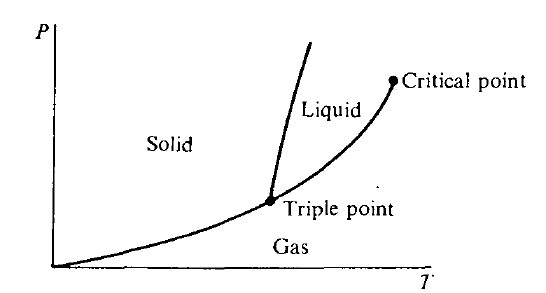
\includegraphics[width=0.5\textwidth]{Immagini/PhaseDiagram.png}
	\caption{}
	\label{fig:phdiagr}
	\vspace{-30pt}
\end{wrapfigure}

Ci sono varie osservazioni da fare:
\begin{itemize}
	\item la più importante è la scelta delle variabili $P-T$, esse sono variabili intensive, e il motivo è chiaro: se la \textit{fase} è caratterizzata dall'uniformità essa non potrà direttamente dipendere da proprietà estensive quali il volume, infatti raddoppiando il sistema (numero di particelle compreso) esso manterrà lo stesso tipo di ordine, sarà solo più grande;
	\item le linee marcate nel diagramma sono note come \textit{linee di coesistenza}, e in quei punti nel sistema sono presenti le due fasi contemporaneamente; essendo oggetti $1$-D sono individuati da una sola variabile, infatti fissata una fra pressione e temperatura l'altra è determinata dalla condizione di coesistenza;
\end{itemize}

\begin{itemize}
	\item il punto di intersezione fra le due linee di coesistenza è detto \textit{punto triplo}, in esso coesistono le tre fasi, ed è individuato da una esatta pressione e temperatura;
	\item la lineaa di coesistenza tra \textit{liquido} e \textit{gas} termina in un punto critico: questo implica che non si può realmente distinguere fra l'uno e l'altro, perché è possibile cambiare fase in modo continuo, aggirando tale punto\footnote{\`E però evidente che se il punto critico è piuttosto distante è abbastanza facile distinguere tra liquido e gas, perché potreste non essere praticamente possibile realizzare un percorso che aggiri il punto critico.}.
\end{itemize}

Si riporta inoltre un altro diagramma, relativo al piano $P-V$:

\begin{figure}[H]
	\centering
	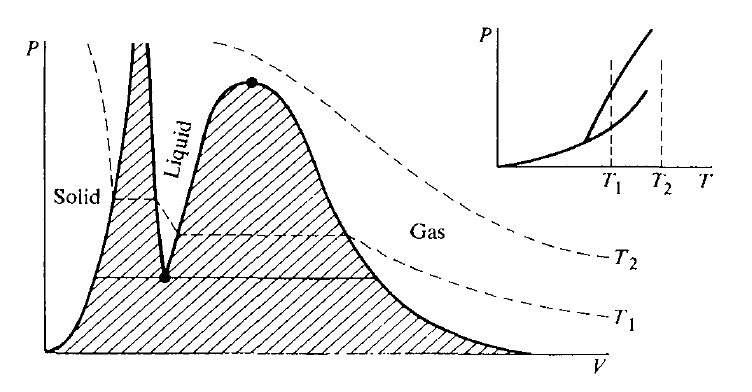
\includegraphics[width=0.7\textwidth]{Immagini/PhasePV.png}
	\caption{}
	\label{fig:phasepv}
\end{figure}

Ciò che si vuole evidenziare di esso è che la \textit{"traiettoria"} delle curve isoterme (tratteggiate in figura) nella regione tratteggiata (regione di coesistenza): esse coincidono con delle isobare, corentemente con quanto descritto a proposito delle curve di coesistenza.
Le variabili $P$ e $T$ non sono quindi sufficienti in questa regione a descrivere il sistema, poiché a $P$ e $T$ fissati sono possibili diversi valori di $V$.

Quello che sta accadendo è che $V$ descrive quanta parte del sistema è in una o in un'altra fase, poiché nella varie fasi cambia il \textit{volume specifico} $V/N$; per cui nella regione ad alto $V$ il sistema sarà prevalentemente nella fase ad alto volume specifico, e viceversa nella regione a basso $V$.

Ci sono altre cose interessanti da notare in questo grafico: la posizione del punto critico e quella del punto triplo, la \textit{separazione} tra solido e liquido, la transizione "diretta" da gas a solido. Si lascia al lettore lo studio di questa proprietà sul diagramma.

\subsubsection{Equazione di Clausius-Clapeyron}

Nella \cref{fig:phdiagr} si può inoltre notare come tutte le curve di coesistenza abbiano derivata sempre positiva. Questa è una proprietà frequente, ma non necessaria.

Il motivo è il seguente, e verrà verificato a posteriori: se l'entropia specifica e il volume specifico crescono in modo concorde da una fase all'altra la pendenza della curva sarà positiva, se discorde sarà negativa.

Intuitivamente ciò che succede è che ad alta temperatura sarà privilegiata la fase più entropica (ha un peso maggiore nell'energia libera di Gibbs) mentre ad alta pressione quella a più alta densità, quindi più basso volume specifico. Se una stessa fase soddisfa entrambi i requisiti allora la pendenza della curva sarà negativa, e la variazione discorde, viceversa nell'altro caso. 
\newline

Per ricavare il risultato precedente si consideri un sistema isolata, costituito da due sottosistemi, che condividono lo stesso volume e lo stesso insieme di particelle, e sono distinti dallo stato: ciascuno rappresenta una diversa fase.

Dalle condizioni di equilibrio ricavate precedentemente si ha $T_1 = T_2$ e $P_1 = P_2$. Un ulteriore condizione si ottiene considerando:
\begin{align*}
\begin{rcases*}
\dd N_1 + \dd N_2 = \dd V = 0\\
\delta F \geq 0
\end{rcases*}
\frac{\partial F}{\partial N_1} = \frac{\partial F_1}{\partial N_1} + \frac{\partial F_2}{\partial N_1} = \frac{\partial F_1}{\partial N_1} - \frac{\partial F_2}{\partial N_2} = 0
\end{align*}

\noindent Perciò $\mu_1 = \mu_2$.

Da questa uguaglianza si può ricavare un'equazione per $P$ e $T$:

\begin{equation*}
\mu_1 (P,T) = \mu_2 (P,T)
\end{equation*}

Per cui si può risolvere per una delle due variabili e ottenere l'equazione esplicita della curva (si noti che se le fasi che coesistono fossero tre ci sarebbe un'altra equazione da soddisfare, cioè l'uguaglianza con $\mu_3$, questo porterebbe ad individuare un unico punto, il punto triplo).

Per ricavarsi l'equazione della curva è quindi necessaria l'espressione esplicita del potenziale chimico in funzione delle due variabili indicate. Questa può essere ricavata da una teoria microscopica delle fasi.

Si può comunque ricavare un utile risultato dalla relazione di Gibbs-Duhem:

\begin{align*}
&\dd \mu_1 = \dd \mu_2 \implies -s_1 \dd T + v_1 \dd P = -s_2 \dd T + v_2 \dd P \implies \\
&\qquad \implies \derivative{ P_0}{T} = \frac{s_2 - s_1}{v_2 - v_1}
\end{align*}

\noindent dove si è usato $s = S/N$ e $v = V/N$, rispettivamente entropia e volume specifici.

In questo ambito si definisce inoltre il \textit{calore latente}:

\begin{defn}[Calore latente]
	\`E una grandezza $\lambda$ delle dimensioni di un'energia (un calore), che caratterizza le transizioni di fase discontinue, cioè quelle in cui è presente una differenza finita di entropia specifica tra le due fasi.
	\begin{equation*}
		\lambda = T(s_2 - s_1) = T \Delta s
	\end{equation*} 
\end{defn}

Alla luce di questa nuova definizione l'equazione di Clausius-Clapeyron è espressa in modo naturale come:

\begin{equation*}
\derivative{ P_0}{T} = \frac{\lambda}{T(v_2 - v_1)}
\end{equation*}

\section{Meccanica Statistica}
\label{sec:statmech}

Il compito della meccanica statistica è principalmente \textit{contare il numero di stati possibili} per un dato macrostato, cioè trovare $\Gamma(E,V,N)$, come indicato nella \cref{sec:entro}.

Da esso infatti sarà possibile trovare l'espressione per l'entropia, e invertendo ques'ultima si avrà l'energia in funzione delle sue variabili proprie, che determina in modo completo la dinamica macroscopica.

In reltà non è conveniente cercare di ottenere $E(S,V,N)$, perché l'entropia non è una variabile così naturale, specie dal punto di vista sperimentale. Si cercherà invece di ottenere la funzione $ F(T,V,N) $, oppure $ \Omega(T,V,\mu) $, le cui variabili proprie risultano molto più intuitive (si ribadisce che l'equazione per la pressione a partire da $ F $ è direttamente l'equazione di stato).

\subsubsection{Derivazione}
Poiché si è interessati a un sistema in cui è fissata la sola temperatura $ T $, o essa e il potenziale chimico $ \mu $, anziché l'energia, si ricorrerà alla descrizione \textit{canonica} introdotta nella \cref{sec:teorpipterm}, nel primo caso; nel caso in cui sia variabile anche il numero di particelle occorre passare alla descrizione \textit{grancanonica}: essa non è una sostanziale novità, infatti è sufficiente partire dal caso canonico, e ammettere che il sistema possa scambiare \textit{particelle} col bagno termico, oltre che energia (in questo contesto infatti il bagno termico viene anche detto \textit{riserva}).
\newline

Si consideri quindi un sistema isolato\footnote{Le cui variabili di equilibrio saranno indicate da uno $0$ a pedice, mentre quelle fuori equilibrio da una $t$ a pedice.}, composto da un piccolo sottosistema\footnote{Le cui variabili saranno disadorne.}, che è ciò che si vuole descrivere, e un bagno termico, detto anche \textit{mezzo}\footnote{Le cui variabili saranno primate.}.
\newline

Il mezzo sarà all'equilibrio, e questo suo stato non è affatto influenzato dalle variazioni nel sottosistema, che risulta troppo piccolo per poterlo perturbare abbastanza da portarlo fuori equilibrio.
Si avrà quindi:
\begin{align*}
&S_t \leq S_0	\qquad \iff \qquad	\Gamma_t \leq \Gamma_0\\
&\dd E' = T \dd S' - P \dd V' + \mu 	\dd N'
\end{align*}

\noindent La prima è data dal secondo principio e la seconda dalla condizione di equilibrio del mezzo (e il primo principio naturalmente). Le variabili del sistema isolato $E_0, V_0, N_0$ sono costanti e esattamente conservate a causa dell'isolamento, perciò le variabili che descrivono lo stato del mezzo dovranno dipendere dallo stato del sottosistema.

Si può considerare il sottosistema contenuto in un volume fissato (qualcosa deve essere fissato per definire in cosa consista il sottosistema). Si userà l'approssimazione che per ogni microstato $\alpha$:
\begin{align*}
&E_\alpha \ll E_0\\
&N_\alpha \ll N_0
\end{align*}

\noindent I possibili microstati in realtà sarebbero tutti, quindi anche quelli in cui l'energia o il numero di particelle del sottosistema siano uguali a quelli dell'intero sistema isolato. L'approssimazione non è così drastica però, infatti la condizione che la temperatura e il potenziale chimico siano fissati dalle proprietà del sistema isolato rende estremamente improbabili i microstati che non rientrano nell'approssimazione effettuata, per cui contribuirebbero comunque in modo trascurabile alla statistica.

Per lo stato fuori equilibrio si avrà:
\begin{align*}
&\Gamma_t = \Gamma \Gamma'\\
&S_t = S + S'
\end{align*}

\noindent e per le probabilità di un singolo microstato del sistema isolato all'equilibrio:

\begin{equation*}
w_{eq} = \frac{1}{\Gamma_0}
\end{equation*}

Se si fissa invece il microstato del sottosistema a essere $\alpha$, si avrà:

\begin{equation*}
\Gamma_{t\alpha} = 1 \cdot \Gamma'_\alpha
\end{equation*}

\noindent poiché il sottosistema è esattamente in uno stato, e quindi la probabilità che si realizza sarà:

\begin{equation*}
w_\alpha = \frac{\Gamma'_{\alpha}}{\Gamma_0}
\end{equation*}

\noindent e il mezzo avrà un'entropia $S'_\alpha \equiv S'(E_0 - E_\alpha, N_0 - N_\alpha)$:
\begin{align*}
&S'_\alpha = k_B \log \Gamma'_\alpha \implies \\
& \qquad \implies S_0 - S'_\alpha = - k_B \log \frac{\Gamma'_{\alpha}}{\Gamma_0} = - k_B \log w_\alpha
\end{align*}

Non è possibile identificare $S_0 - S'_\alpha$ con l'entropia del sottosistema (che è nulla perché si trova in uno stato determinato). Tale differenza è frutto del fatto che il sistema non è all'equilibrio, avendo imposto il vincolo che il sottosistema sia in $\alpha$.

Si può ottenere però l'entropia del sottosistema all'equilibrio sottraendo a quella totale quella del mezzo, mediata su tutti i possibili microstati\footnote{Che coincide con mediare la quantità trovata nell'espressione precedente}.
\begin{align*}
S &= \overline{S_0 - S'_\alpha} = S_0 - \overline{S'_\alpha} = \overline{- k_B \log w_\alpha} = \\
&= - \sum_{\alpha} w_\alpha \log w_\alpha
\end{align*}

Quest'ultima espressione è definibile per ogni distribuzione di probabilità discreta, e nel contesto della teoria dell'informazione è chiamata \textit{entropia di Shannon}.
Tornando un passo indietro si era ottenuto:
\begin{align*}
	&w_\alpha = \exp \left(- \frac{S_0 - S_\alpha}{k_B}\right) = A \exp \left(\frac{S_\alpha}{k_B}\right) \qquad \qquad \qquad A = cost.\\
	&\qquad \qquad S'_\alpha = S'(E_0 - E_\alpha, N_0 - N_\alpha) \simeq S'(E_0, N_0) - \partfix{S'}{E'}{V',N'} E_\alpha - \partfix{S'}{N'}{V',E'} N_\alpha =\\
	&\qquad \qquad \qquad = cost. - \frac{E_\alpha}{T} + \frac{\mu N_\alpha}{T} \implies\\
	&\implies w_\alpha = \frac{1}{\mathcal{Z}} \exp \left(- \frac{E_\alpha - \mu N_\alpha}{k_BT}\right)
\end{align*}

\noindent Nell'espressione precedente si è sfruttata l'approssimazione prima discussa per calcolare l'entropia del mezzo al prim'ordine, e si è infine trovata un'espressione per le probabilità $w_\alpha$ in funzioni delle variabili macroscopiche del sottosistema.

La quantità $\mathcal{Z}$ è molto importante, e viene chiamata \textit{funzione di granpartizione}.

\begin{defn}[Funzione di granpartizione]
	La \textit{funzione di granpartizione} è la quantità:
	\begin{equation*}
	\mathcal{Z} = \sum_{\alpha} \exp \left(- \frac{E_\alpha - \mu N_\alpha}{k_BT}\right)
	\end{equation*}
	
	Essa è una funzione della temperatura $T$ e del potenziale chimico $\mu$.
\end{defn}

Si definisce analogamente la \textit{funzione di partizione}, nel caso in cui il numero di particelle sia fissato:

\begin{defn}[Funzione di partizione]
	La \textit{funzione di partizione} è la quantità:
	\begin{equation*}
	Z = \sum_{\alpha} \exp \left(- \frac{E_\alpha}{k_BT}\right)
	\end{equation*}
	
	Essa è una funzione della temperatura $T$.
\end{defn}

Si ricava infine una proprietà fondamentale delle quantità ora definite:

\begin{align*}
S &= - \sum_{\alpha} w_\alpha \log w_\alpha =\\
&= k_B \log \mathcal{Z} \sum_{\alpha} w_\alpha + \frac{1}{T} \sum_{\alpha} w_\alpha E_\alpha - \frac{\mu}{T} \sum_{\alpha} w_\alpha N_\alpha =\\
&= k_B \log \mathcal{Z} + \frac{E - \mu N}{T} \implies\\
\implies & - k_B T \log \mathcal{Z} = E - T S - \mu N = F - \mu N = \Omega
\end{align*}

Allo stesso modo si dimostra $F = E - T S = - k_B T \log Z$.

\subsection{Densità di stati}

Si osservi che si è ottenuta la probabilità di un singolo stato $\alpha$ del sottosistema dallo studio dell'entropia del mezzo. Quest'ultimo tuttavia non distingue i vari stati del sottosistema, ma rileva solo la sua energia e il numero di particelle (da qui in avanti il numero di particelle sarà considerato fisso).

Questo si risolve nel fatto che:
\begin{equation*}
\Gamma'_{E_\alpha} = \Gamma'_\alpha
\end{equation*}
\noindent cioè l'entropia del mezzo è la stessa anche nel caso in cui si specifichi solo l'energia. Ciò che cambia è l'entropia del sottosistema, per cui:
\begin{align*}
&\Gamma_{tE_\alpha} = \rho_{E_\alpha} \Gamma'_\alpha \implies \\
\implies w&(E_\alpha) = \frac{\Gamma_{tE_\alpha}}{\Gamma_0} = \frac{\rho_{E_\alpha} \Gamma'_\alpha}{\Gamma_0} = \rho_{E_\alpha} w_\alpha
\end{align*}

\noindent dove si è usata la quantità $\rho_{E_\alpha}$, detta \textit{densità di stati}.

\begin{defn}[Densità di stati]
	La \textit{densità di stati} $\rho_{E_\alpha}$ è definita:
	\begin{itemize}
		\item per valori discreti dell'energia: è il numero di stati per livello energetico, cioè è la funzione che associa ad ogni livello la sua \textit{degenerazione};
		\item per valori continui: è propriamente la densità degli stati in funzione dell'energia, cioè, se integrata su un certo intervallo, corrisponde al numero di stati in quel dato intervallo.
	\end{itemize}
\end{defn}

\noindent La densità di stati è determinata unicamente dalla \textit{legge di dispersione}, di cui si è già trattato nella \cref{sec:teorpipterm}.

Il risultato trovato per la probabilità in funzione dell'energia è intuitivo: poiché la probabilità di un microstato dipende solo dalla sua energia allora la probabilità di una certa energia $E_\alpha$ corrisponde alla probabilità di un qualunque microstato con energia $E_\alpha$ moltiplicata per il numero di microstati con energia $E_\alpha$, cioè la densità di stati.

\begin{oss}
	La probabilità in energia è una quantità più naturale che la probabilità per i singoli microstati. Infatti è atteso che un sistema a una data temperatura $T$ abbia un'energia pari a $\sim k_B T$. La probabilità degli autostati è però esponenzialmente depressa, per cui sembrano favoriti gli stati a bassa energia a qualunque temperatura.
	
	Quello che accade è che la densità di stati aumenta con l'energia,  si annulla per energia nulla (in realtà va a $1$, se discreta\footnote{E per basse energie è sempre discreta, perché comincia la zona dello spettro discreto per gli atomi.}, seguendo il terzo principio) e va a $\infty$ per energie grandi\footnote{Si assume sempre che lo spettro delle particelle non è limitato dall'alto.}. 
	
	\`E la combinazione di questi due effetti che porta $w(E_\alpha)$ a formare un picco, centrato approssimativamente in $k_B T$, e la cui larghezza si annulla per sistemi molto grandi (si veda la \cref{sec:fluct}).
\end{oss}

Poiché i livelli energetici di un corpo macroscopico sono molto ravvicinati si possono sostituire le somme con integrazioni (per una discussioni più dettagliata si veda più avanti la \cref{sec:sumasint}).

Si otterrà perciò che la media di un'osservabile $f$ è data da:

\begin{align*}
\bar{f} &= \int_{0}^{\infty} f(\mathcal{E}) w(\mathcal{E})\dd \mathcal{E} = \frac{1}{Z} \int_{0}^{\infty} f(\mathcal{E}) \rho(\mathcal{E}) e^{-\mathcal{E}/k_B T}\dd \mathcal{E}\\
& Z = \int_{0}^{\infty} \rho(\mathcal{E}) e^{-\mathcal{E}/k_B T}\dd \mathcal{E}\
\end{align*}

\noindent in cui $Z$ è ancora la funzione di partizione, ma espressa anch'essa in forma d'integrale.

Si è usato il simbolo $\mathcal{E}$ per evidenziare che si tratta di una variabile continua, diversamente da prima.

\begin{note}
	Integrando fino a $\infty$ non si rispetta l'approssimazione sotto cui si erano ricavate le probabilità per i singoli stati, e le altre espressioni che ne scaturivano. Questa in realtà non è una nuova approssimazione, ma è consistente con la vecchia: si era ricavato infatti che la probabilità per gli stati era soppressa esponenzialmente ad alta energia, e questo giustifica l'estensione del limite di integrazione, anzi è concettualmente più corretta.
	
	Infatti gli stati che erano stati trascurati esistono, solo non contribuiscono statisticamente, che è esattamente quello che sta accadendo nell'integrazione.
\end{note}

La nuova espressione per l'energia libera sarà quindi anch'essa in forma di integrale (deriva direttamente da quella di $Z$). Si è quindi ridotto l'intero problema della meccanica statistica a trovare la funzione $\rho(\mathcal{E})$, infatti:

\begin{itemize}
	\item tramite integrazione $\rho(\mathcal{E})$ determina $F(T,V)$;
	\item dall'espressione dell'energia libera si può ricavare tutta la termodinamica.
\end{itemize}

Per la gioia del lettore: i passi avanti che si sono fatti sono solo formali, infatti il problema iniziale era trovare $\Gamma(E,V,N)$, adesso si chiama $\rho(\mathcal{E}, N)$, ma il problema è sempre un conteggio.

\subsubsection{Approssimazione di Einstein}

Si ha che, anche per la probabilità in funzione dell'energia si ottiene un'espressione analoga in funzione dell'entropia.
\begin{align*}
&w(E_\alpha) = \frac{\rho_{E_\alpha} \Gamma'_\alpha}{\Gamma_0} = \exp \left(- \frac{S_0 - S_t(E_\alpha)}{k_B}\right) = A \exp \left(\frac{S_t(E_\alpha)}{k_B}\right) \qquad \qquad A = cost.\\
\end{align*}

Al posto dell'energia in realtà può esserci una qualunque quantità $x$ che influenzi il bagno termico (lo si può ricavare ripercorrendo il modo in cui si era introdotta l'energia). Si avrà dunque:
\begin{align*}
&S'_x \simeq S'_{\bar{x}} - \partdev{S'}{x}(\bar{x} - x)\\
&w(x) = A_{x_0} \exp \left(\frac{S_t(x)}{k_B}\right)
\end{align*}

\noindent Imponendo la condizione di massimo per l'entropia totale si ha:
\begin{align*}
S_t(x) \simeq S_t(\bar{x}) + &\partfix{S_t}{x}{x=\bar{x}}(x - \bar{x}) + \frac{1}{2} \partfix{^2 S_t}{x^2}{x=\bar{x}}(x - \bar{x})^2 = S_t(\bar{x}) - \beta(x - \bar{x})^2 \implies\\
&\implies w(x) = D \exp \left(-\frac{\beta(x - \bar{x})^2}{k_B}\right)
\end{align*}

\noindent in cui $\beta \geq 0$ e la costante $D$ è fissata dalla normalizzazione:
\begin{equation*}
\int w(x) \dd x = 1 = D \sqrt{\frac{2 \pi k_B}{\beta}}
\end{equation*}

L'approssimazione effettuata corrisponde a considerare una forma gaussiana per $w(x)$ (cioè: tutti i picchi sono una campana), e quindi com'è noto tutti i contributi vengon dalla zona attorno a $\bar{x}$.

\subsection{Proprietà di $Z$ e $\mathcal{Z}$}

Dalla funzione di partizione si può ricavare direttamente l'energia. Il modo più facile per vederlo è introdurre la variabile $\beta = (k_B T)^{-1}$ e derivare l'espressione di $Z$:
\begin{align*}
Z &= \int_{0}^{\infty} \rho(\mathcal{E}) e^{-\beta \mathcal{E}}\dd \mathcal{E} \implies\\
\implies - \partdev{Z}{\beta} &= \int_{0}^{\infty} \mathcal{E}\rho(\mathcal{E}) e^{-\beta \mathcal{E}}\dd \mathcal{E}\ = Z \mathcal{E} \implies\\
\implies E &= - \partdev{\log Z}{\beta}
\end{align*}

Che si può trasformare in un'espressione esplicita della temperatura semplicemente applicando \textit{chain rule}:
\begin{align*}
E &= - \partdev{\log Z}{T} \partdev{T}{\beta} = k_B T^2 \partfix{\log Z}{T}{V,N}
\end{align*}

\noindent Per completezza: si può ottenere la stessa espressione ricavando $F$ da $Z$, e $E$ da $F$ (dalla definizione di $F$ si ha che $E = F + T S$) e tenendo conto che anche $S$ può essere ricavata da $F$ tramite una derivata in $T$.


\subsection{Particelle identiche}
\label{sec:idpart}

\subsection{Integrazione sugli stati}
\label{sec:sumasint}

\subsection{Fluttuazioni}
\label{sec:fluct}

\chapter{Gas perfetto}
\label{chap:gas}

% !TEX encoding = UTF-8
% !TEX TS-program = pdflatex
% !TEX root = ../Appunti.tex

\section{Gas ideale}

Le definizioni di gas perfetto e ideale sono state date nel primo capitolo, e sono rispettivamente la \cref{def:perfgas} e la \cref{def:idgas}.

Si ricorda che la condizione di idealità era data da:
\begin{equation*}
e^{\mu/k_B T} \ll 1
\end{equation*}

Calcolando il valore del numero di particelle per mezzo della densità di stati:
\begin{equation*}
N = \sum_{\textbf{q}} \overline{n_{\textbf{q}}} = \int \exp \left(- \frac{\varepsilon - \mu}{k_B T}\right) \rho(\varepsilon) \dd \varepsilon = \frac{V}{\Lambda^3} e^{\mu/k_B T}
\end{equation*}
\begin{equation*}
\Lambda = \frac{2\pi \hbar}{\sqrt{2\pi m k_B T}}
\end{equation*}

Per cui la condizione di idealità può essere riespressa in funzione della densità $\rho$ del sistema:
\begin{equation*}
	e^{\mu/k_B T} = \Lambda^3 \frac{N}{V} = \Lambda^3 \rho	\qquad \implies \qquad \rho \ll \frac{1}{\Lambda^3}
\end{equation*}

Per cui $\Lambda(T)$ fornisce il parametro su cui valutare l'idealità del gas, e dipende dalla temperatura $T$ del sistema, perciò è detta \textit{lunghezza d'onda termica} di De Broglie.

Essa è detta lunghezza d'onda perché si può immaginare di raccogliere le onde piane in pacchetti localizzati, e l'ordine di grandezza sarebbe quello di $\Lambda$, infatti per il principio di indeterminazione la minima indeterminazione possibile sarà proporzionale a $\hbar/p$, ma $p$ tipico sarà determinato dall'energia, che è quella termica, per cui $p \sim (2 m k_B T)^{1/2}$.

Per cui $\Lambda^3$ è la dimensione tipica dei pacchetti d'onda, e la condizione di idealità corrisponde quindi a richiedere che i pacchetti risultino puntiformi rispetto alle distanze tipiche del sistema, in modo che gli effetti quantistici non siano coinvolti nella dinamica.

Si possono inoltre ricavare le altre proprietà del gas ideale a partire dalla energia libera di Gibbs:
\begin{align*}
	\mu &= - k_B T \log \frac{k_B T}{P \Lambda^3}\\
	G &= N\mu = - N k_B T \log \frac{k_B T}{P \Lambda^3}
\end{align*}

In particolare per l'entropia e le due capacità termiche:
\begin{align*}
	S &= -Nk_B \log \frac{N}{V} + \frac{3}{2} N k_B \log k_B T + N k_B \left(\frac{5}{2} + \frac{3}{2}\log \frac{m}{2\pi \hbar^2}\right)\\
	C_P &= \frac{5}{2} N k_B \qquad C_V = \frac{3}{2} N k_B
\end{align*}

Nel precedente capitolo le proprietà del gas perfetto erano state discusse usando l'approccio canonico, e quindi ricavandosi l'energia libera $F$:
\begin{equation*}
	F_c = - N k_B T \log \left(\frac{V}{\Lambda^3}\right) + k_B T \log N!
\end{equation*}

Il problema è che l'energia libera, calcolata a partire dall'energia libera ricavata nell'approccio grancanonico, è apparentemente differente:
\begin{equation*}
F_{gc} = G - PV = - N k_B T \log \left(\frac{V}{N \Lambda^3}\right) - N k_B T
\end{equation*}

\noindent Per cui:
\begin{equation*}
	F_{gc} - F_c = k_B T (N \log N - N - \log N!)
\end{equation*}
ma questa differenza si annulla asintoticamente con $N \rightarrow \infty$, per l'approssimazione di Stirling. 
Questo risultato era prevedebile: nell'approccio canonico il sistema ha un numero di particelle fissato, mentre nell'approccio grancanonico il numero di particelle può fluttuare, ma le fluttuazioni relative si annullano asintoticamente.

\begin{ex}[Approssimazione di Stirling]
	L'approssimazione di Stirling si può ricavare sviluppando $\log N!$ in forma di serie, e approssimandolo con un integrale su un supporto opportuno.
\end{ex}

\paragraph{Deviazioni dall'idealità} Si nota che la questione di un gas perfetto e non ideale è apparentemente quasi accademica. Infatti le tipiche condizioni sotto cui un gas è perfetto sono le stesse sotto cui è ideale:
\begin{description}
	\item[bassa densità] in modo tale che la distanza tra le particelle sia grande rispetto alla scala tipica dell'interazione (nel caso dell'idealità il confronto era da farsi con la scala di lunghezza data dall'indeterminazione quantistica);
	\item[alta temperatura] l'energia delle interazioni dev'essere piccola rispetto all'altra scala di energia: l'energia termica (nel caso dell'idealità la temperatura entra in gioco nel determinare le scale di lunghezza).
\end{description}

Per cui tipicamente quando vengono meno le condizioni di idealità vengono meno anche quelle di perfezione. Anzi, spesso la condizione di gas non interagente è la prima ad essere violata (la scala dell'indeterminazione quantistica è più piccola di quella delle interazioni).

In realtà sono noti esempi in cui il gas si comporta come non ideale, anche se le interazioni continuano a non essere sostanzialmente rilevanti (elettroni in un metallo tipicamente, o in parte è anche il caso delle stelle di neutroni, in cui però sono coinvolti effetti relativi alla gravità).

Per il momento si procede semplicementestudiando la questione.

\section{Statistiche di Bose-Einstein e Fermi-Dirac}
\label{sec:BFstat}

In meccanica quantistica l'\textit{identicità} delle particelle ha un significato molto più forte che in meccanica classica: essa è strettamente correlata direttamente al \textit{principio di indeterminazione}.

Infatti l'identificazione di una particella implica la localizzazione nello spazio fisico, ma questo porta a una grande indeterminazione sull'impulso, che comporta che tale identificazione venga persa subito dopo. In altri termini: mentre in meccanica classica le particelle potevano essere identiche, ma data una configurazione iniziale era possibile \textit{seguire le traiettorie} e riconoscere a un dato istante che una data particella fosse quella che era partita in un dato punto, questa possibilità si perde in meccanica quantistica.
\newline

\`E noto, dalla meccanica quantistica, che il modo corretto di trattare le particelle identiche è quello di assegnare al sistema a molti-corpi funzioni d'onda che siano \textit{completamente simmetriche o antisimmetriche} per scambio di particelle.

In particolare: 
\begin{itemize}
	\item se le funzioni d'onda possono essere solo completamente simmetriche, cioè invarianti per permutazioni, le particelle vengono dette \textit{bosoni}, e si distribuiscono secondo la statistica di Bose-Einstein;
	\item se le funzioni d'onda possono essere solo completamente antisimmetriche, cioè sotto permutazione vengono moltiplicate per il segno di essa ($-1$ per le dispari, $1$ per le pari), vengono dette \textit{fermioni}, e soddisfano la statistica di Fermi-Dirac.
\end{itemize}

L'effetto dei due vincoli è quello di consentire, per ogni stato di singola particella, tutti i possibili \textit{numeri d'occupazione} nel caso dei bosoni, mentre esclusivamente $0,1$ per i fermioni (in fatti se ci fosse più di una particella nello stesso stato scambiando due si troverebbe che la funzione d'onda è pari a meno se stessa, e quindi nulla).
\newline

Si considera quindi il caso di un gas perfetto nei due scenari descritti.

Si noti che le probabilità di occupazione di uno stato di singola particella in un gas perfetto sono note dalla generalizzazione dell'ensemble di Gibbs al caso microcanonico, e sono:
\begin{equation*}
w_{\textbf{q}} = \exp \left[-\frac{(\varepsilon_{\textbf{q}} - \mu) n_{\textbf{q}}}{k_B T}\right]
\end{equation*}
\textit{indipendentemente} dalle considerazioni sull'\textit{identicità} delle particelle.

\subsection{Fermi-Dirac}

Si esamina il comportamento del gas perfetto applicando il metodo suggerito in \cref{sec:idpart}: lo studio dei numeri di occupazione degli stati di singola particella.
La funzione di granpartizione del singolo stato è dunque:
\begin{equation*}
\Omega_{\textbf{q}} = - k_B T \log \left[1 + \exp \left(-\frac{\varepsilon_{\textbf{q}} - \mu}{k_B T}\right)\right]
\end{equation*}
poiché l'antisimmetrizzazione delle funzioni d'onda esclude la presenza di più particelle nello stesso stato, quindi i numeri di occupazione maggiori di $1$, e di conseguenza la somma è troncata.

Questo risultato è formalmente identico a quello trovato nel caso di particelle classiche, ma vi è una differenza sostanziale è \textit{esatto}. 
Infatti nel caso classico era il risultato di una approssimazione, e quindi aveva dei limiti sulla validità.

Questo fatto garantisce il corretto limite classico, nel caso in cui le condizioni dell'approssimazione precedente siano nuovamente verificate.
\newline

Studiando il numero di occupazione medio del singolo stato, si ottiene:
\begin{equation*}
\overline{n_{\textbf{q}}} = - \partdev{\Omega_{\textbf{q}}}{\mu} = \frac{\exp\left[(\varepsilon_{\textbf{q}} - \mu)/k_B T\right]}{1 + \exp\left[(\varepsilon_{\textbf{q}} - \mu)/k_B T\right]} = \frac{1}{\exp\left[(\varepsilon_{\textbf{q}} - \mu)/k_B T\right] + 1}
\end{equation*}
per cui il numero medio di occupazione è sempre minore di $1$ (nel limite classico $\ll 1$).

Per ottenere l'intera funzione di granpartizione e il numero di particelle si sommano le precedenti quantità su tutti gli stati possibili.

\subsection{Bose-Einstein}
Si applica lo stesso metodo descritto nel caso precedente, però vengono meno i vincoli imposti dall'antisimettrizzazione (la funzione d'onda è simmetrica anche se tutte le particelle sono nello stesso stato, anzi, lo è in modo naturale).

La funzione di granpartizione del singolo stato è dunque:
\begin{equation*}
\Omega_{\textbf{q}} = - k_B T \log \left[\sum_{n_{\textbf{q}}=0}^{N} \exp \left(-\frac{(\varepsilon_{\textbf{q}} - \mu )n_{\textbf{q}}}{k_B T}\right)\right] \simeq - k_B T \log \left[\sum_{n_{\textbf{q}}=0}^{\infty} \exp \left(-\frac{(\varepsilon_{\textbf{q}} - \mu) n_{\textbf{q}}}{k_B T}\right)\right]
\end{equation*}
Si nota che l'approssimazione considerata non è altro che il limite termodinamico, inoltre è ben verificata anche per $N$ finiti, infatti la probabilità $w_{\textbf{q}}$ è comunque soppressa esponenzialmente con il numero di occupazione.

Si è approssimato con una serie perché essa è una serie geometrica \footnotemark, e quindi si sa calcolare esattamente, e si trova:
\begin{equation*}
\Omega_{\textbf{q}} = - k_B T \log \left[\frac{1}{1 - \exp[-(\varepsilon_{\textbf{q}} - \mu)/k_B T]}\right] = k_B T \log \left[1 - \exp(-\frac{\varepsilon_{\textbf{q}} - \mu}{k_B T})\right]
\end{equation*}

Perché la serie non diverga è necessario però che:
\begin{equation*}
\mu < \varepsilon_{\textbf{q}} ~~\forall \textbf{q} \qquad \iff \qquad \mu < \varepsilon_0
\end{equation*}
dove si è indicato con $\varepsilon_0$ l'energia del fondamentale. Nel caso di un gas perfetto in cui il volume in cui è contenuto è molto più grande rispetto alla scala della lunghezza d'onda termica l'energia del fondamentale è trascurabile, per cui si richiede $\mu < 0$.
\footnotetext{Se ci fosse bisogno di ricordarlo:
\begin{equation*}
\sum_{n=0}^{\infty} x^n = \frac{1}{1-x}
\end{equation*}
}

Studiando il numero di occupazione medio del singolo stato, si ottiene:
\begin{equation*}
\overline{n_{\textbf{q}}} = - \partdev{\Omega_{\textbf{q}}}{\mu} = \frac{1}{ \exp\left[(\varepsilon_{\textbf{q}} - \mu)/k_B T\right] - 1}
\end{equation*}
si noti che in questo caso non ci sono limiti al numero di occupazione possibile.

Come nel caso del gas di Fermi per ottenere l'intera funzione di partizione o il numero di particelle si somma su tutti gli stati possibili.

Anche in questo caso nel limite di alte temperature e basse densità si recupera il caso classico; infatti espandendo il $\log$ in $\Omega_{\textbf{q}}$ si recupera il segno di differenza dal caso del gas di Fermi, e quindi coincidendo col gas di Fermi coincide col caso classico.

\section{Gas poco degenere}
\label{sec:fewdegas}

\subsubsection{Integrazione sugli stati}
\`E ancora possibile integrare sugli stati, anziché sommare, nelle condizioni in cui si presentano effetti quantistici rilevanti?

\noindent La risposta è quasi sempre sì. Non è vero per ogni regime, ma le condizioni che portano a commettere un grosso errore effetuando l'integrazione sono ancora più stringenti di quelle che portano al manifestarsi della natura quantistica della materia.

Infatti il criterio per valutare l'errore commesso nell'integrazione si basa su quanto siano ravvicinati gli stati, cioè se la differenza in energia tra gli stati (detta in inglese \textit{energy gap}) sia molto minore della scale energetiche di interesse del problema.

In particolare confrontando tale differenza con l'energia termica si ottiene la condizione:
\begin{equation*}
	\frac{\hbar^2}{2m}\left(\frac{2\pi}{L}\right)^2
\end{equation*}
dove $L$ sono è la scala tipica delle dimensioni lineari del sistema.

\begin{es}
Per dare un'idea degli ordini di grandezza in gioco nel caso di $L \sim \unit{1}{\centi\meter}$ e $m \sim \unit{10^{-24}}{\gram}$ - l'ordine di grandezza della massa dell'atomo di idrogeno - si ha che la temperatura fissata dall'\textit{energy gap} è pari a $\sim \unit{10^{-13}}{\kelvin}$. Se invece si usa la massa dell'elettrone $m \sim \unit{10^{-27}}{\gram}$ si ottiene una temperatura $\sim \unit{10^{-10}}{\kelvin}$.
In entrambi i casi sono limiti facilmente rispettati.
\end{es}

\subsubsection{Correzioni al caso classico}

\paragraph{Degenerazione di spin} C'è un ulteriore considerazione da fare, legata ai gradi di libertà di \textit{spin}. Nel caso più semplice in assenza di campo (che è quello che si andrà qui a considerare) l'effetto è quelo di inserire una degenerazione ulteriore nei livelli energetici:
\begin{equation*}
g = 2S + 1
\end{equation*}
per cui lo spazio delle fasi diventa:
\begin{equation*}
g \frac{\dd ^3 p \dd ^3 r}{(2\pi \hbar)^3}
\end{equation*}
e anche nella densità di stati compare quindi il fattore $g$.

In seguito tale fattore sarà considerato $g=1$ per i bosoni e $g=2$ per i fermioni, in quanto il caso tipico di applicazione saranno fermioni di spin $1/2$ o bosoni a spin nullo.

\paragraph{Equazione di stato} Si procede esaminando l'insorgere di effetti quantistici in un gas classico che comincia ad allontanarsi dal regime di idealità. Per fare ciò si espandano al secondo ordine nella condizione di idealità $e^{\mu/k_B T}$ le espressioni trovate per $\Omega$\footnote{Il segno superiore si riferisce a Fermi-Dirac, quello inferiore a Bose-Einstein}:
\begin{align*}
	\Omega &\simeq \mp \sum_{\textbf{q}} \log(1 \pm \exp[-\frac{\varepsilon_{\textbf{q}} - \mu}{k_B T}]) = -k_B T \sum_{\textbf{q}} \exp(-\frac{\varepsilon_{\textbf{q}} - \mu}{k_B T}) \pm \frac{k_B T}{2} \sum_{\textbf{q}} \exp(-2\frac{(\varepsilon_{\textbf{q}} - \mu)}{k_B T}) = \\
	&= \Omega_{class} \pm \frac{k_B T}{2} \exp(\frac{2\mu}{k_B T})\sum_{\textbf{q}} \exp(-\frac{2\varepsilon_{\textbf{q}} }{k_B T})
\end{align*}
dove $\Omega_{class}$ è la funzione di granpartizione classica, che come detto nella \cref{sec:BFstat} costituisce il prim'ordine della funzione di granpartizione in entrambi i casi quantistici.

Si deve quindi valutare la somma, e in accordo a quanto detto prima lo si fa integrando:
\begin{equation*}
\sum_{\textbf{q}} \exp(-\frac{2\varepsilon_{\textbf{q}} }{k_B T}) \simeq \int_0^{\infty} \rho(\varepsilon) \exp(-\frac{2\varepsilon }{k_B T}) \dd \varepsilon = \left(\frac{1}{2}\right)^{3/2 } \int_0^{\infty} \rho(2\varepsilon) \exp(-\frac{2\varepsilon }{k_B T}) \dd (2\varepsilon)
\end{equation*}
dove si è usato il fatto che $\rho(\varepsilon) \propto \varepsilon^{1/2}$, per cui la correzione è:
\begin{equation*}
\pm \left(\frac{1}{2}\right)^{5/2}k_B T e^{2\mu/k_B T}  \int_0^{\infty} \rho(\varepsilon) \exp(-\frac{\varepsilon }{k_B T}) \dd \varepsilon
\end{equation*}
mentre il termine dominante è:
\begin{equation*}
\Omega_{class} = -k_B T \sum_{\textbf{q}} \exp(-\frac{\varepsilon_{\textbf{q}} - \mu}{k_B T}) \simeq - k_B T e^{\mu/k_B T}  \int_0^{\infty} \rho(\varepsilon) \exp(-\frac{\varepsilon }{k_B T}) \dd \varepsilon
\end{equation*}

Si ottiene infine:
\begin{equation*}
	\Omega \simeq \Omega_{class}\left[1 \mp \frac{e^{\mu/k_B T}}{2^{5/2}}\right]
\end{equation*}
e quindi, considerando che $\Omega = - PV$ e $\Omega_{class} = - N k_B T$, l'equazione di stato è:
\begin{equation*}
	PV = N k_B T \left[1 \mp \frac{e^{\mu/k_B T}}{2^{5/2}}\right]
\end{equation*}

Per interpretare tale correzione si deve considerare il procedimento utilizzato: usando $\Omega$ si è considerato l'approccio grancanonico, in cui $T,V$ e $\mu$ sono fissati, ma $N$ è libero. Per cui la correzione trovata non è direttamente una correzione alla pressione, ma una correzione a $P/N$.

\noindent Per capire cosa stia succedendo al gas è più facile chiedersi cosa accade alla pressione se $T,V$ e $N$ sono costanti, in modo da trovare esplicitamente la nuova pressione, così da confrontarla col caso classico.

Per raggiungere questo obiettivo è naturale passare per l'energia libera $F$, dato che sono le sue variabili proprie.
Si ha dalla \cref{sec:thermquant}:
\begin{equation*}
(\delta \Omega)_{T, V, \mu} = (\delta F)_{T,V,N}
\end{equation*}
e usando la notazione:
\begin{align*}
\Omega(T,V,\mu) &= \Omega_{class} + (\delta \Omega)_{T, V, \mu}\\
F(T,V,N) &= F_{class} + (\delta F)_{T, V, N}
\end{align*}
si ha:
\begin{equation*}
\delta \Omega = \mp \Omega_{class}\frac{e^{\mu/k_B T}}{2^{5/2}} = \pm N k_B T \frac{e^{\mu/k_B T}}{2^{5/2}}
\end{equation*}

Per trovare la correzione a $F$ si deve esprimere $\mu$ nell'espressione precedente in funzione di $T,V,N$. Si sostituisce il valore:
\begin{equation*}
\mu_{class} = -k_B T \log\frac{V}{N \Lambda^3}
\end{equation*}
in quanto includendo in $\mu$ qualunque correzione, già a partire dal prim'ordine, si otterebbero correzioni di ordine superiore al primo nella pressione.

Si trova quindi per $F$:
\begin{equation*}
F = F_{class} \pm \frac{N^2 k_B T \Lambda^3}{2^{5/2} V}
\end{equation*}
e infine per la pressione:
\begin{equation*}
P = - \partdev{F}{V} = P_{class} \pm \frac{N^2 k_B T \Lambda^3}{2^{5/2} V^2} = \frac{N k_B T}{V} \left(1  \pm \frac{N\Lambda^3}{2^{5/2} V}\right)
\end{equation*}

Come atteso le correzioni sono piccole nella quantità $\Lambda^3 / \rho = N\Lambda^3 / V$, che evidenziano come gli effetti quantistici derivino dall'\textit{overlap} del supporto dei pacchetti d'onda delle particelle.

Osservando il segno delle correzioni si nota che:
\begin{itemize}
	\item per il \textbf{gas di Fermi} il \textit{principio di esclusione di Pauli} agisce come una sorta di forza repulsiva, aumentando la pressione del gas rispetto al caso classico;
	\item per il \textbf{gas di Bose} l'assenza di restrizioni agisce come una interazione attrattiva fra le particelle, diminuendo la pressione.
\end{itemize}

\section{Gas di Fermi molto degenere: elettroni nei metalli}
La descrizione del comportamento degli elettroni nei metalli, e quindi delle peculiari proprietà che distinguono i metalli dagli altri elementi, è uno dei grandi successi della teoria del gas di Fermi degenere.
\newline

Si esamina quindi cosa succede ai fermioni nel limite opposto a quello classico, cioè il limite di bassa temperatura.
Lo stato "asintotico" è relativamente facile da esaminare: si impone $T=0$, e quindi che il sistema stia nel fondamentale, esattamente.

La struttura del fondamentale a molti corpi è piuttosto semplice: si comincia a riempire gli stati di singola particella a partire dal fondamentale e salendo via via, scegliendo sempre quello a più bassa energia disponibile, fino a esaurimento delle particelle. Per particelle di spin $S$ si deve ricordare di considerare l'ulteriore degenerazione $g_S$ degli stati.

L'impulso relativo allo stato a più alta energia riempito è detto \textit{impulso di Fermi} $p_F$, e nello spazio degli impulsi di singola particella il fondamentale a molti corpi si struttura come una sfera di raggio $p_F$ al cui interno gli stati sono tutti occupati da $g$ particella ciascuno, e al cui esterno sono vuoti\footnote{Invece nello spazio degli impulsi a molti corpi, in cui il gas classico era un guscio sferico di stati, il gas di Fermi collassa \textit{"in un singolo punto"}, dato che lo stato è completamente determinato. In realtà non è esattamente un punto in cui collassa, ma una sovrapposizione quantistica (un singolo punto non sarebbe isotropo, e non ci sono direzioni privilegiate).}.

Lo stesso risultato può essere ottenuto esaminando l'espressione per il numero medio di occupazione: quanto $T\rightarrow 0$ allora gli stati in cui $\varepsilon_{\textbf{q}} > \mu$ tendono a un numero medio di occupazione nullo, mentre se $\varepsilon_{\textbf{q}} < \mu$ allora $\overline{n_{\textbf{q}}} \rightarrow 1$.

\begin{figure}[t]
	\centering
	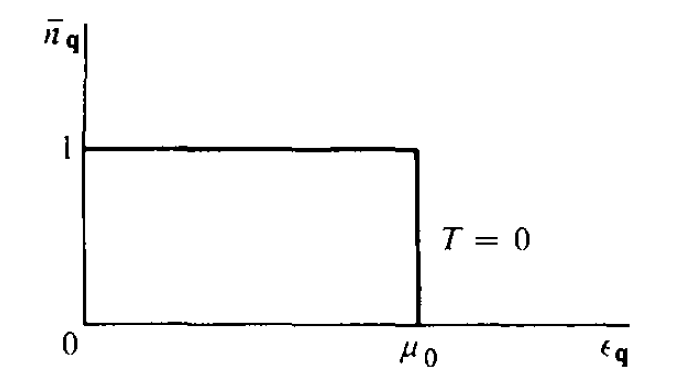
\includegraphics[width=0.5\textwidth]{Immagini/FermiStep.png}
	\caption{}
	\label{fig:fermistep}
\end{figure}

La funzione $n_{\textbf{q}} (\varepsilon_{\textbf{q}})$ diventa quindi una funzione a gradino (vedi \cref{fig:fermistep}), in cui il punto di frontiere è $\varepsilon_{\textbf{q}} = \mu_0$, cioè il potenziale chimico a $T=0$, che è fissato dall'equazione:
\begin{equation*}
N = \lim_{T\rightarrow 0} \sum_{\textbf{q}} \frac{1}{\exp\left[(\varepsilon_{\textbf{q}} - \mu)/k_B T\right] + 1}
\end{equation*}

Anche in questo caso le somme saranno convertite in integrali, e i livelli energetici saranno considerati un insieme continuo. La giustificazione qui non può più essere data dal confronto con la scala di energia termica, che qui è nulla, ma la scala di energia rilevante qui è proprio quella indotta da $\mu_0$, ed è rispetto ad essa che i livelli energetici sono fini, ed è strettamente connesso al fatto che si sta considerando una quantità macroscopica di particelle.

Si ha dunque che l'equazione diventa\footnote{Usando il solito \textit{teorema fisico} che afferma che limiti e integrali commutano. Formalmente non funziona, ma praticamente sì. La giustificazione migliore è che le funzioni per cui fallisce hanno un comportamento particolare, concettualmente allargano infinitamente il loro supporto \textit{efficace} nel passaggio al limite, e sono una classe ristretta.}:
\begin{equation*}
N = \lim_{T\rightarrow 0} \int_{0}^{\infty} \frac{\rho(\varepsilon)}{\exp\left[(\varepsilon_{\textbf{q}} - \mu)/k_B T\right] + 1} \dd \varepsilon = \int_{0}^{\mu_0} \rho(\varepsilon) \dd \varepsilon
\end{equation*}
dove si è usato che il numero di occupazione diventa la funzione a gradino al limite.

Invece di integrare la densità di stati si può ottenere $N$ direttamente considerando che è il numero di celle unitarie di spazio delle fasi racchiuso in un volume fisico $V$ e in una sfera di raggio $p_F$ nello spazio degli impulsi, non dimenticando la degenerazione di spin. Si ottiene quindi:
\begin{equation*}
N = \frac{gV \frac{4}{3} \pi p_F^3}{(2\pi \hbar)^3}
\end{equation*}
Da cui si ottiene:
\begin{align*}
p_F &= 2\pi \hbar \left(\frac{N}{V} \frac{3}{4\pi g}\right)^{1/3}\\
\mu_0 &= \frac{p_F^2}{2m} = \frac{(2\pi \hbar)^2}{2m} \left(\frac{N}{V} \frac{3}{4\pi g}\right)^{2/3}
\end{align*}

Si nota che contrariamente al caso del gas classico il potenziale chimico $\mu_0$ è qui positivo: infatti non è possibile aggiungere particelle a energia nulla, ma solo a energia $\geq \mu_0$, inoltre non c'è bisogno di fare alcuna correzione per la variazione di entropia, che è nulla prima e dopo l'inserimento.

Il potenziale chimico $\mu_0$ è noto come \textit{energia di Fermi} $\varepsilon_F$. \`E anche nota la temperatura di Fermi $T_F$, definita da $k_B T_F = \varepsilon_F$.
\newline

Poiché anche nel caso quantistico la densità di stati di singola particella in energia è proporzionale a $\varepsilon^{1/2}$ allora:
\begin{align*}
	\bar{\varepsilon} = \frac{\int_{0}^{\varepsilon_F} \varepsilon \rho(\varepsilon) \dd \varepsilon}{\int_{0}^{\varepsilon_F} \rho(\varepsilon) \dd \varepsilon} = \frac{\int_{0}^{\varepsilon_F} \varepsilon^{3/2} \dd \varepsilon}{\int_{0}^{\varepsilon_F} \varepsilon^{1/2} \dd \varepsilon} = \frac{\frac{2}{5} \varepsilon_F^{5/2}}{\frac{2}{3} \varepsilon_F^{3/2}} = \frac{3}{5} \varepsilon_F
\end{align*}
e di conseguenza l'energia totale:
\begin{equation*}
E = \frac{3}{5} N \varepsilon_F = \frac{3(2\pi \hbar)^2}{10m} \left(\frac{N}{V} \frac{3}{4\pi g}\right)^{2/3} N
\end{equation*}
poiché l'entropia è nulla allora l'energia libera è pari all'energia $E=F$, e dunque per la pressione si ha:
\begin{equation}
P = - \partfix{F}{V}{T,N} =\partfix{E}{V}{N} = \frac{2}{3} \frac{E}{V}
\end{equation}
Questa pressione finita temperatura nulla è la conseguenza estrema della forza efficace repulsiva tra fermioni che si iniziava a manifestare già in prossimità del limite classico (vedi \cref{sec:fewdegas}).

Inoltre il risultato trovato conferma la previsione generale, vista nella \cref{sec:idpart}, che per un gas perfetto $ E = \frac{3}{2} PV$, che dipende solo dalla legge di dispersione e dalla definizione di pressione, mentre ciò che differisce nei due casi è proprio l'energia: per un gas ideale a $T=0$ l'energia è nulla, e quindi anche la pressione.

\paragraph{Basse temperature} Per temperature piccole, ma non nulle, ci si aspetta che il comportamento del gas sia prossimo a quello a $T=0$, quindi si studierà tale limite in modo perturbativo.

La condizione di basse temperature è che:
\begin{equation*}
T \ll T_F
\end{equation*}

Un valore tipico per $T_F$ si può ottenere considerando l'espressione per $\varepsilon_F$ e valori tipici per le varie grandezze:
\begin{itemize}
	\item per la massa delle particelle si considera quella dell'elettrone;
	\item per la degenerazione di spin si pone $g=2$, cioè spin $1/2$;
	\item per la densità, che è la densità degli elettroni di conduzione dei metalli, si considera quella del rame, conduttore comune (in ogni caso varia di meno di un ordine di grandezza fra i vari metalli);
\end{itemize}
Il valore che si ottiene per la temperatura di Fermi è $T_F = \unit{8.5}{\kelvin}$, mentre il punto di fusione del rame è $\sim \unit{10^3}{\kelvin}$, per cui finché il rame è solido gli elettroni soddisfano pienamente il limite di bassa temperatura.
\newline

Ciò che accade è che alzando la temperatura da $0$ gli elettroni sul guscio esterno acquistano un energia dell'ordine di $k_B T$, ma quelli in profondità nel \textit{mare di Fermi} non possono fare altrettanto, perché tutti gli stati accessibili tramite eccitazione termica sono già occupati.

Quindi solo gli elettroni sul guscio contribuiscono alle deviazioni rispetto al comportamento a $T=0$, e sono una frazione piccola del totale, dell'ordine di $T/T_F$ (la palla che costituisce il mare di Fermi nello spazio degli impulsi è tridimensionale, quindi non ci sono comportamenti peculiari causati da sfere di dimensionalità alta).

\begin{figure}[h!]
	\centering
	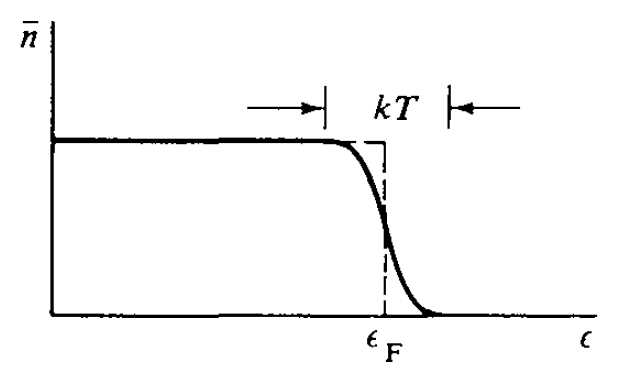
\includegraphics[width=0.5\textwidth]{Immagini/FStepT.png}
	\caption{}
	\label{fig:fstepT}
\end{figure}

La forma che assume adesso il numero medio di occupazione è simile alla precedente, ma appare più \textit{smussata} (non ci possono essere discontinuità a temperatura finita), come è mostrato in \cref{fig:fstepT}. 
Si noti che la zona interessata ha uno spessore dell'ordine di $k_B T$.
\newline

Il modello di conduzione precedente all'introduzione dei gas di Fermi era quello di Drude, esso però presentava un problema fondamentale: se gli elettroni costituivano un gas non-interagente anche loro dovevano avere una loro capacità termica, proporzionale al numero di gradi di libertà (per il teorema di equipartizione), e misurandola si è potuto fissare un limite superiore al numero di elettroni in un metallo. Il limite così trovato risultava troppo ridotto: un tale numero di elettroni non erano sufficienti a dare conto delle proprietà di conduzine dei metalli.

Questo dilemma può essere risolto dal modello proposto dal gas di fermioni: tutti gli elettroni contribuiscono alla conduzione elettrica, perché l'effetto del campo è quello di spostare l'intera sfera di Fermi (la perdita di isotropia è giustificata dalla direzione individuata dal campo), mentre la conduzione termica coinvolge solo gli elettroni del guscio, cioè una frazione dell'ordine $T/T_F$ del totale, dando ragione della capacità termica ridotta rispetto al grande numero di particelle.

Ci sono però dei punti da chiarire prima di potere applicare il modello del gas di Fermi alla conduzione:
\begin{itemize}
	\item il gas che si sta considerando non è ideale, ma è pur sempre perfetto: come può esserlo un gas costituito da particelle cariche? La risposta è che gli elettroni in moto in un metallo sono immersi in una regione di carica positiva costituita dagli ioni (il metallo è globalmente neutro), per cui essi tendono a "schermarsi" con le cariche positive e costituire dei portatori efficaci, che appaiono neutri gli uni agli altri; più avanti si inserirà questo effetto nel modello;
	\item la stessa distribuzione di Fermi rende più improbabili le collisioni: gli elettroni in profondità nel mare di Fermi non possono collidere, perché il risultato della collisione sarebbe quello di raggiungere un nuovo stato, ma quelli immediatamente attorno sono occupati, e quindi le collisioni soppresse;
	\item un'ultima obiezione potrebbe essere che non si stanno considerando le collisioni con gli elementi della struttura cristallina del metallo: gli ioni positivi; il motivo per cui vengono trascurate è che gli elettroni non sono elementi localizzati nel metallo, ma gli stati di singola particella costituiti da onde, la cui lunghezza è determinata dall'impulso, ed è molto più grande della spaziatura fra gli atomi per la maggioranza degli stati coinvolti; delle onde così lunghe non possono quindi accorgersi significativamente della struttura granulare del reticolo (questo punto sarà affrontato con maggiore dettaglio nel \cref{chap:crystals}, in cui si tratterà dei cristalli).
	
	Si anticipa che legge di dispersione degli elettroni in un metallo in effetti è piuttosto diversa da quella di un gas perfetto. Quest'ultima è:
	\begin{equation*}
	\varepsilon = \frac{\hbar^2 q^2}{2 m^\ast}
	\end{equation*}
	dove con $m^\ast$ è indicata la massa efficace dei portatori dovuta alla schermatura discussa al primo punto, ed è un poco maggiore di quella degli elettroni a causa della carica positiva addizionale.
	La differenza nelle leggi di dispersione è illustrata in 
\end{itemize}

\begin{figure}[t]
\centering
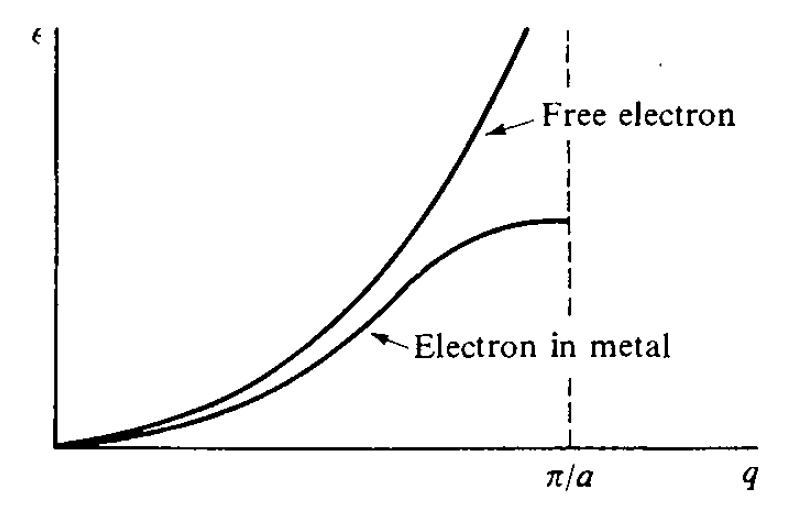
\includegraphics[width=0.5\textwidth]{Immagini/ElectronsDispersion.png}
\caption{}
\label{fig:elecdisp}
\end{figure}

Si studiano ora le proprietà termiche del gas perfetto di Fermi, partendo dalla funzione di granpartizione:
\begin{equation*}
\Omega = - k_B T \sum_{\textbf{q}} \log \left[1 + \exp \left(-\frac{\varepsilon_{\textbf{q}} - \mu}{k_B T}\right)\right] = - k_B T \int_{0}^{\infty} \rho(\varepsilon)\log \left[1 + \exp \left(\frac{\mu - \varepsilon}{k_B T}\right)\right] \dd \varepsilon
\end{equation*}
Che può essere integrata per parti, oppure si può prendere una scorciatoia e considerare che (finché $\varepsilon \propto p^2$) $E = -\frac{3}{2} \Omega$, e quindi:
\begin{equation*}
\Omega = =  -\frac{2}{3} E = -\frac{2}{3} \int_{0}^{\infty} \rho(\varepsilon)\bar{n}(\varepsilon)\dd \varepsilon = - \frac{2}{3} \frac{4\pi V g \sqrt{2} m^{3/2}}{\hplanck^3} \int_{0}^{\infty}\frac{\varepsilon^{3/2} \dd \varepsilon}{e^{(\varepsilon - \mu)/k_BT} +1}
\end{equation*}
Per valutare questa espressione si deve quindi eseguire l'integrale di una funzione che è molto vicina al gradino.
Si può quindi trattare il problema perturbativamente e trovare quale sia la correzione $\delta I$ al valore dell'integrale $I_0$ a temperatura nulla:
\begin{align*}
I = I_0 + \delta I \qquad I_0 &= \int_{0}^{\mu} f(\varepsilon) \dd \varepsilon\\
I= \int_{0}^{\infty} f(\varepsilon) \bar{n}(\varepsilon) \dd \varepsilon &= \int_{0}^{\infty}  \frac{f(\varepsilon)}{e^{(\varepsilon - \mu)/k_BT} +1} \dd \varepsilon
\end{align*}
\`E importante ricordare che la variazione in $T$ è fatta a $\mu$ costante, quindi $N$ può cambiare (se si impone il contrario il valore di $I_0$ dipenderà dalla temperatura, ma si può fare).

Sviluppando quindi $I$ in $T=0$ si ha:
\begin{equation*}
I = I_0 + \partfix{I}{T}{T=0} T + \frac{1}{2} \partfix{^2 I}{T^2}{T=0} T^2 + ~\cdots
\end{equation*}

La questione fondamentale qui è a quale ordine si trova il primo termine non nullo (dopo quello all'ordine zero ovviamente), poiché il comportamento termico sarà dominato da esso. Il risultato è che tale termine è quello al second'ordine, mentre il primo si annulla.

Il motivo per cui il termine al prim'ordine è nullo è sostanzialmente che le particelle in più con $\varepsilon_{\textbf{q}} > \mu$, appena sopra tale limite, danno un contributo a $\Omega$ quasi uguale a quello dato dalle particelle con $\varepsilon_{\textbf{q}}$ appena inferiore a $\mu$, che vengono a mancare rispetto al caso del gradino. La situazione è illustrata in \cref{fig:stepsmooth}.

\begin{figure}[b]
	\centering
	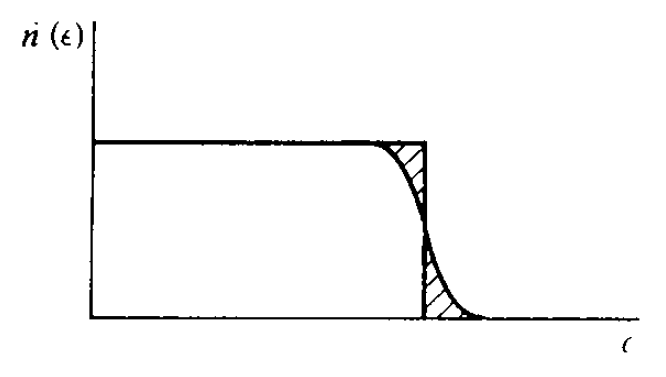
\includegraphics[width=0.5\textwidth]{Immagini/SmoothStep.png}
	\caption{}
	\label{fig:stepsmooth}
\end{figure}

Più in dettaglio si ha che il numero di particelle a una certa energia $\varepsilon$ è dato da $\rho(\varepsilon)\bar{n}(\varepsilon)$, e poiché nella zona attorno a $\mu$ la densità degli stati $\rho(\varepsilon)$ varia relativamente poco l'area tratteggiata in \cref{fig:stepsmooth} corrisponde quasi al numero di particelle che vengono promosse, e quindi il fatto che le due aree si compensino riflette il fatto che il numero di particelle è quasi conservato.
\newline

Si passa quindi alla valutazione quantitativa. Sia:
\begin{equation*}
	z = \frac{\varepsilon - \mu}{k_B T}
\end{equation*}

Si possono definire due funzioni di $z$, $g_0(z)$ e $g_1(z)$, che rappresentino le aree tratteggiate, cioè la differenza tra il gradino e il numero medio di occupazione a temperatura finita, e che quindi siano significativamente diverse da $0$ solo in un intorno di $z=0$, come mostrato in \cref{fig:stepdiffunc}.

\begin{figure}[t]
	\centering
	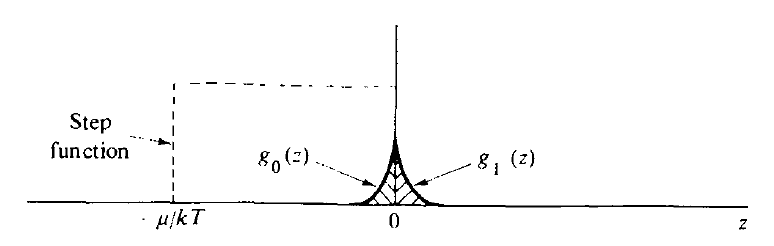
\includegraphics[width=0.7\textwidth]{Immagini/SmoothStepDifferences.png}
	\caption{}
	\label{fig:stepdiffunc}
\end{figure}

Si ottiene quindi:
\begin{equation*}
\delta I = \int_{-\infty}^{\infty} f(\varepsilon)[g_1(z) - g_0(z)] \dd \varepsilon = \int_{-\infty}^{\infty} f(\mu + k_B T z)[g_1(z) - g_0(z)] \kt \dd z
\end{equation*}
i limiti di integrazione considerati non introducono un ulteriore approssimazione perché al di fuori della regione di integrazione precedente il valore delle funzioni $g$ è praticamente nullo ovunque.

Si espande quindi $f$ in $z=0$ e si sostituisce in $\delta I$:
\begin{align*}
f(\mu + \kt z) &= f(\mu) + \kt z \partfix{f}{\varepsilon}{\varepsilon = \mu} + \cdots = f(\mu) + \kt z f'(\mu) + \cdots\\
\delta I &= \kt f(\mu) \int_{-\infty}^{\infty} [g_1(z) - g_0(z)] \dd z + (\kt)^2 f'(\mu) \int_{-\infty}^{\infty} z[g_1(z) - g_0(z)] \dd z
\end{align*}
il primo termine è quindi effettivamente proporzionale alla differenza di aree. Inoltre, se il primo termine si annulla sarà perché la funzione è approssimativamente dispari, e quindi si annulleranno tutti i termini di ordine dispari. D'altro canto il secondo termine non può annullarsi perché è sempre positivo.

Si esaminano quindi le funzioni $g$:
\begin{align*}
g_1(z) &= \frac{1}{e^z + 1}	\qquad (z \geq 0)\\
g_0(z) &= 1 - \frac{1}{e^z + 1} = \frac{e^z}{e^z + 1} = \frac{1}{1 + e^{-z}} \qquad (z < 0)
\end{align*}
ottenute considerando che $g_1$ coincide sostanzialmente con $\bar{n}$ e $g_0$ con $1 - \bar{n}$, per entrambi sul loro supporto.

Da queste espressioni si ottiene quindi:
\begin{align*}
	\int_{-\infty}^{\infty} [g_1(z) - g_0(z)] \dd z &= \int_{0}^{\infty} g_1(z) \dd z - \int_{-\infty}^{0} g_0(z) \dd z = \int_{0}^{\infty} \frac{\dd z}{e^z + 1} - \int_{-\infty}^{0} \frac{\dd z}{1 + e^{-z}} =\\
	&= \cdots ~+ \int_{+\infty}^{0} \frac{\dd z}{1 + e^{z}} = \cdots ~- \int_{0}^{\infty} \frac{\dd z}{1 + e^{z}} = 0
\end{align*}
mentre per il secondo termine:
\begin{equation*}
\int_{-\infty}^{\infty} z [g_1(z) - g_0(z)] \dd z = 2 \int_{0}^{\infty} \frac{z\dd z}{e^z + 1} = \frac{\pi^2}{6}
\end{equation*}

La formula per l'espansione di $I$ al quart'ordine\footnote{Qui abbiamo motivato, ed è sufficiente, il secondo} è:
\begin{equation*}
I = \int_{0}^{\mu} f(\varepsilon) \dd \varepsilon +  \frac{\pi^2}{6} f'(\mu) (\kt)^2 + \frac{7\pi^4}{360} f'''(\mu) (\kt)^4 + \cdots
\end{equation*}
e infine per la funzione di granpartizione:
\begin{equation*}
\Omega = - \frac{2}{3} \frac{4\pi V g \sqrt{2} m^{3/2}}{\hplanck^3}\left[\frac{2}{5}\mu^{5/2} + \frac{\pi^2}{4} \mu^{1/2} (\kt)^2\right]
\end{equation*}

Da quest'ultima è possibile ricavare il numero di particelle:
\begin{equation*}
N = - \partfix{\Omega}{\mu}{V,T} = - \frac{2}{3} \frac{4\pi V g \sqrt{2} m^{3/2}}{\hplanck^3}\left[\mu^{3/2} + \frac{\pi^2}{8} \frac{(\kt)^2}{\mu^{1/2}}\right]
\end{equation*}
e dall'espressione del numero di particelle a temperatura nulla $N_0$ si ha che:
\begin{align*}
N_0 &= \frac{2}{3} \frac{4\pi V g \sqrt{2} m^{3/2} \mu^{3/2}}{\hplanck^3}\\
N &= N_0\left[1 + \frac{\pi^2}{8} \left(\frac{\kt}{\mu}\right)^2\right]
\end{align*}

Questo è il risultato trovato considerando il caso grancanonico, in cui $\mu$ è fisso e il numero totale di particelle $N$ può cambiare attingendo alla riserva,
Si può invece considerare $N$ fisso e $\mu$ variabile, che è una situazione che si presenta frequentemente, specialmente in ambito sperimentale (ma non necessariamente, il campione ad esempio potrebbe essere parte di un circuito elettrico).

Il numero delle particelle sarà quindi:
\begin{equation*}
N = N_0\left[1 + \frac{\pi^2}{8} \left(\frac{\kt}{\mu}\right)^2\right]\left(\frac{\mu}{\mu_0}\right)^{3/2}
\end{equation*}
poiché $N_0 \propto \mu^{3/2}$, in modo da riprodurre il risultato precedente. Imponendo quindi $N = N_0$ si trova $\mu_0$:
\begin{equation*}
\mu \simeq \frac{\mu_0}{\left[1 + {\pi^2}/{8} \left({\kt}/{\mu_0}\right)^2\right]^{2/3}} \simeq \mu_0 \left[1 - \frac{\pi^2}{12} \left(\frac{\kt}{\mu_0}\right)^2\right]
\end{equation*} 
in cui nella prima uguaglianza si è posto $\mu = \mu_0$ nel membro di destra, per limitarsi all'approssimazione al primo ordine non nullo, mentre nella seconda uguaglianza si sviluppato il denominatore.

Era prevedibile, ma non ovvio, che il potenziale chimico: ad alte temperature si recupera il limite classico, per cui $\mu$ deve diventare negativo e grande con l'alzarsi della temperatura.
\newline

A partire dalla funzione di granpartizione si può anche ricavare l'entropia:
\begin{equation*}
S = - \partfix{\Omega}{T}{V, \mu} = \frac{4\pi V g \sqrt{2} m^{3/2}}{\hplanck^3} \frac{\pi^2}{3} \mu^{1/2} k_B^2 T 
\end{equation*}
che è la funzione $S(T,V,\mu)$, piuttosto che $S(T,V,N)$; ma si sa che una variazione di $ \mu $ con $  N $ costante è dell'ordine $ T^3 $, quindi trascurabile rispetto alle altre.

Si può quindi scrivere:
\begin{equation*}
S = \frac{\pi^2}{2} N k_B \frac{T}{T_F}
\end{equation*}
e quindi ottenere la capacità termica a volume costante:
\begin{equation*}
C_V = T \partfix{S}{T}{V} = \frac{\pi^2}{2} N k_B \frac{T}{T_F}
\end{equation*}
in accordo a quanto affermato precedentemente sul fatto che per i fenomeni termici sono rilevanti solo gli elettroni del guscio, con una frazione tipica data da $T/T_F$

Si trova che il risultato sperimentale è in accordo con l'andamento lineare, ma differisce nelle costanti, infatti:
\begin{align*}
\frac{C_V}{N \kt} &= 0.8 \cross 10^{-4} \qquad (\text{experimental})\\
\frac{C_V}{N \kt} &= 0.6 \cross 10^{-4} \qquad (\text{predicted})
\end{align*}

Questa differenza può essere colmata in base alla considerazione fatta all'inizio della sezione sulla massa efficace dovuta alla schermatura, infatti $C_V \propto T_F^{-1} \propto m$ per cui una massa $m^\ast \simeq 1.3 m$ da ragione del valore leggermente più alto ottenuto sperimentalmente.
\newline

Nella discussione fatta ci sono alcuni punti che sono stati trascurati:
\begin{itemize}
	\item i cristalli non sono isotropi, per cui il mare di Fermi anziché avere la forma di una sfera nello spazio degli impulsi a forme più complesse, e l'impulso di Fermi può dipendere in generale dalla direzione lungo cui lo si valuta;
	\item gli elettroni non interagiscono con gli atomi del cristallo nelle loro posizioni di equilibrio, ma possono interagire con le impurità del cristallo e con il moto di eccitazine termica del reticolo (i fononi).
\end{itemize}
Inoltre potrebbe essere naturale essere scettici riguardo al ruolo della massa efficace, in particolare essa appare come un parametro libero che viene fissato ad hoc per rendere la teoria in accordo con la realtà sperimentale.
Si è però provato che non è esattamente così: studiando il moto degli elettroni in un cristallo sotto l'azione di un campo magnetico si è riusciti a determinare che gli elettroni si comportano, per distanze dell'ordine del libero cammino medio, come particelle cariche in un ciclotrone, con una frequenza:
\begin{equation*}
\omega_c = \frac{e H}{m^\ast c}
\end{equation*}
in questo modo si è misurato in modo indipendente il valore di $m^\ast$.

Il valore trovato in questo modo dipende dalla direzione, a causa proprio dell'anisotropia dei cristalli, ma una volta opportunamente mediato esso è in ottimo accordo con i dati ottenuti dallo studio delle capacità termiche.

\section{Gas di Bose molto degenere: condensati di Bose-Einstein}

Le equazioni trovate nella \cref{sec:BFstat} per il gas di Bose sono estremamente simili in forma a quelle relative al gas di Fermi. I risultati a cui conducono sono però completamenti differenti.
\newline

Si inizia studiando il numero di particelle in un gas di Bose, dato da:
\begin{equation*}
N = \sum_{\textbf{q}}  \frac{1}{ \exp\left[(\varepsilon_{\textbf{q}} - \mu)/k_B T\right] - 1}
\end{equation*}
e considerando che a temperatura finita i la spaziatura tra i livelli è piccola in confronto all'energia termica (le grandezze che vanno confrontate sono la lunghezza d'onda termica con le dimensioni lineari del sistema) si può immediatamente convertire in un integrale:
\begin{equation*}
N =  \frac{4\pi V g \sqrt{2} m^{3/2}}{\hplanck^3} \int_{0}^{\infty}  \frac{\varepsilon^{1/2} \dd \varepsilon}{ \exp\left[(\varepsilon - \mu)/k_B T\right] - 1}
\end{equation*}

Inoltre nel caso del gas di Bose il potenziale chimico è strettamente negativo (al contrario nel caso dei fermioni era positivo).

Si consideri ora la situazione di un gas in un contenitore a  $V$ fissato e in contatto con un bagno termico, che quindi fissa $ T $. Si consideri che il sistema non si ain grado di scambiare particelle con una riserva, e quindi $N$ è fissato, ma con la possibilità di aggiungere particelle dall'esterno (trovando nuovi stati di equilibrio di volta in volta).

L'unica variabile libera nell'equazione scritta per $ N $ è $ \mu $, e $ N(\mu) $ è una funzione crescente. Poiché $\mu$ deve rimanere negativo è lecito chiedersi se esitìstono valori finiti di $ N $ per cui il potenziale chimico raggiunge il suo limite. Si impone quindi $ \mu = 0$ e si calcola il numero totale di particelle:
\begin{align*}
N &=  \frac{4\pi V g \sqrt{2} m^{3/2}}{\hplanck^3} (\kt)^{3/2} \int_{0}^{\infty}  \frac{x^{1/2} \dd x}{ e^x - 1}\\
&\int_{0}^{\infty}  \frac{x^{1/2} \dd x}{ e^x - 1} \simeq 2.31 \simeq \frac{\sqrt{\pi}}{2} \cdot 2.612
\end{align*}
ottenendo quindi una densità critica di particelle, o una temperatura critica (se si immagini di abbassare la temperatura a densità costante):
\begin{align*}
\left(\frac{N}{V}\right)_c &= \frac{2.612}{\Lambda^3}\\
T_c &= \frac{1}{2.31 m k_B} \left(\frac{N}{V}\right)^{2/3} \frac{(\hplanck)^2}{(4\pi \sqrt{2})^{2/3}}
\end{align*}
La presenza di una densità critica, espressa direttamente come funzione di $\Lambda$, rende conto del fatto che le particelle non possono più essere localizzate senza sovrapporsi quantisticamente.
\newline

Il problema è quindi il seguente: non ci sono ragioni evidenti per cui il sistema non possa contenere ulteriori particelle oltre le densità critica, a $ T $ e $ V $ fissati, ma poiché il potenziale chimico non può più crescere il conteggio rimane fisso al valore trovato per $ \mu = 0 $.

La soluzione può essere compresa per analogia con un problema noto: in un gas ideale (ad esempio azoto N$_2$, a una temperatura di $ ~\unit{60}{\kelvin} $, appena sopra al punto triplo) $N = (V/\kt) P$, per cui a $ V $ e $ T $ fissati la pressione dovrebbe essere direttamente proporzionale al numero di particelle, ma sperimentalmente anche aumentando $ N $ a un certo punto la pressione si assesta su un valore costante: il gas sta subendo una transizione di fase, e la curva si assesta sulla pressione di vapore e le nuove particelle sono bilanciate da quelle che passano alla fase liquida. In \cref{fig:gastoliquid} si riporta il comportamento descritto.

\begin{figure}[t]
	\centering
	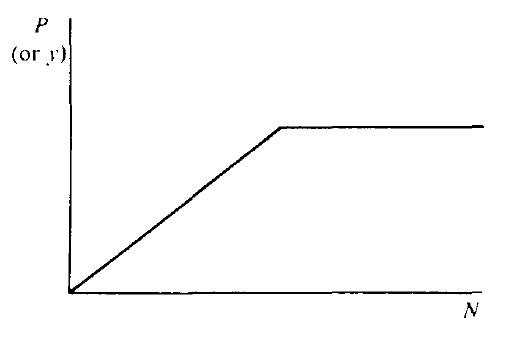
\includegraphics[width=0.5\textwidth]{Immagini/GasToLiquid.png}
	\vspace{-10pt}
	\caption{}
	\label{fig:gastoliquid}
	\vspace{-10pt}
\end{figure}

Si ottiene una figura analoga se si riporta su un grafico il caso del gas di Bose, mantenendo in ascissa $ N $ e ponendo in ordinata:
\begin{equation*}
	y =  \int_{0}^{\infty}  \frac{\varepsilon^{1/2} \dd \varepsilon}{ \exp\left[(\varepsilon - \mu)/k_B T\right] - 1}
\end{equation*}

La domanda diventa quindi: perché il conteggio delle particelle sta perdendo traccia di alcune di esse? Si riesamina quindi il procedimento adoprato.
\begin{itemize}
	\item Potrebbe essere a causa dll'approssimazione fatta integrando sugli stati, anziché sommare; essa è giustificata se il sistema soddisfa:
	\begin{equation*}
		\kt \gg \frac{\hbar^2}{2m} \left(\frac{2\pi}{L}\right)^2
	\end{equation*}
	Si sostituisce quindi la temperatura critica $ T_c $, e poiché $L^2 = V^{2/3}$ il risultato dipende solo dal numero di particelle:
	\begin{equation*}
	N^{2/3} \gg \frac{2.31(4\pi\sqrt{2})^{2/3}}{2}
	\end{equation*}
	ma il secondo membro è una costante dell'ordine dell'unità, perciò per qualunque numero macroscopico di particelle l'approssimazione è ben verificata.
	
	\item Potrebbe essere dovuto della densità di stati (e lo è); nel ricavare la densità di stati si è considerata una particella libera nel vuoto, ma questa è solo un'approssimazione se il volume in cui è confinata è finito.
	
	Gli stati quindi non sono realmente stati del continuo, ma discreti, per cui la densità di stati dovrebbe prevedere la presenza di uno stato anche a energia nulla \footnote{quasi in realtà, ma tende a $0$ con le dimensioni del sistema}, cioè il fondamentale. 
	
	Questo non ha creato problemi nel gas ideale e in quello di fermi: nel primo il numero di occupazione di ogni stato è piccolo per ipotesi, e nel secondo è $\leq g$ (la degenerazione di spin), per cui trascurare uno stato non può portare a effetti statisticamente rilevanti.
	
	Per il gas di Bose invece:
	\begin{equation*}
		\overline{n_0} = \frac{1}{e^{-\mu/\kt} - 1} \qquad \implies \qquad \overline{n_0} \simeq - \frac{\kt}{\mu} \qquad (\mu \rightarrow 0)
	\end{equation*}
	perciò quando il potenziale chimico si annulla il numero di particelle nel fondamentale diventa macroscopico, e si può identificare proprio con il fondamentale la nuova fase in equilibrio con il gas di Bose, ritrovando le particelle mancanti nel conteggio.
	
	Tale fase è detta \textit{condensato di Bose-Einstein}.
\end{itemize}

\subsubsection{Proprietà del condensato di Bose-Einstein}

Le particelle che non sono nel fondamentale sono tutte correttamente incluse nel conteggio fatto per $ N $. Chiameremo ora questo numero $ N^\star $, per distinguerlo dal numero complessivo di particelle del sistema, che sarà sempre $ N $.
Si ha quindi:
\begin{equation*}
N^\star = \int_{0}^{\infty}  \frac{\rho(\varepsilon) \dd \varepsilon}{ e^{\varepsilon/k_B T} - 1} = N \left(\frac{T}{T_C}\right)^{3/2}
\end{equation*}
mentre per le particelle nel fondamentale si ha:
\begin{equation*}
	N_0 = N - N^\star = N \left[1 - \left(\frac{T}{T_C}\right)^{3/2}\right]
\end{equation*}

L'energia del gas è tutta nelle particelle $ N^\star $, essendo le altre nel fondamentale, e quindi a energia nulla.
\begin{equation*}
	E = \int_{0}^{\infty}  \frac{\varepsilon \rho(\varepsilon) \dd \varepsilon}{ e^{\varepsilon/k_B T} - 1} = \frac{4\pi V g \sqrt{2} }{\hplanck^3} (m\kt)^{3/2} \kt \int_{0}^{\infty}  \frac{x^{3/2} \dd x}{ e^x - 1}
\end{equation*}

\begin{note}[Integrali notevoli]
	Tutti gli integrali nella forma in cui è posto quello nell'espressione precedente possono essere valutati per mezzo di \textit{funzioni speciali}:
	\begin{equation*}
		\int_{0}^{\infty}  \frac{x^n \dd x}{ e^x - 1} = \Gamma(n+1) \zeta(n+1)
	\end{equation*}
	dove $ \Gamma(\cdot) $ è la funzione \textit{gamma di Eulero} e $ \zeta(\cdot) $ è la funzione \textit{zeta di Riemann}.
\end{note}

Nel caso in esame si ha:
\begin{equation*}
	\int_{0}^{\infty}  \frac{x^{3/2} \dd x}{ e^x - 1} = \frac{3\sqrt{\pi}}{4} \cdot 1.341
\end{equation*}
per cui l'energia è:
\begin{equation*}
	E = 0.770 \kt N^{\star} = 0.770 \kt N  \left(\frac{T}{T_C}\right)^{3/2}
\end{equation*}
perciò la dipendenza dalla temperatura dell'energia è $ E \propto T^{5/2} $. Conseguentemente la capacità termica è:
\begin{equation*}
	C_V = \partfix{E}{T}{V,N} = 1.9 k_B N  \left(\frac{T}{T_C}\right)^{3/2} = 1.9 N^\star k_B 
\end{equation*}
e quindi dal punto di vista della capacità termica il comportamento della parte eccitata non è molto diverso da quello del gas ideale, in cui $C_V = 1.5 N k_B$.

\begin{figure}[t]
	\centering
	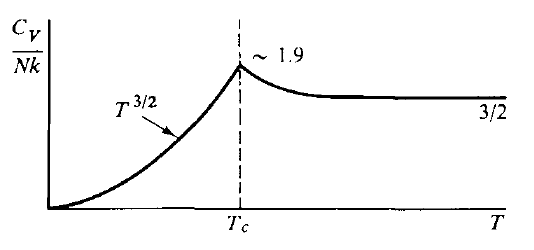
\includegraphics[width=0.6\textwidth]{Immagini/BoseThermalCapacity.png}
	\vspace{-10pt}
	\caption{}
	\label{fig:thermcapbose}
	\vspace{-10pt}
\end{figure}

Si riporta il grafico della capacità termica in funzione della temperatura, in esso sono chiari i seguenti andamenti:
\begin{itemize}
	\item per temperature inferiori alla temperatura critica la capacità termica per singola particella va come $ T^{3/2} $, cioè è proporzionale alla frazione di particelle non condensate;
	\item per temperature molto maggiori della temperatura critica la capacità termica per singola particella tende ad assestarsi su un valore costante, cioè $ 1.5 k_B $, il valore del gas ideale;
	\item per temperature maggiori alla temperatura critica, avvicinandosi ad essa, il comportamento del gas si fa meno ideale, e inizia ad agire la forza efficace tra bosoni, per cui la capacità termica sale leggermente oltre il suo valore ideale a causa di tali interazioni efficaci, fino al valore di $ 1.9 k_Bf $.
\end{itemize}

\subsection{Approfondimenti sui condensati}
Ci sono due ulteriori argomenti elementari d'interesse legati alla condensazione di Bose:
\begin{itemize}
	\item lo studio e la classificazione della transizione di fase;
	\item la condensazione nello spazio fisico.
\end{itemize}

Il primo punto è connesso ad alcuni aspetti della teoria generale sulle transizioni di fase, cioè l'ordine della transizione: la condensazione è effettivamente una transizione del primo ordine, con un calore latente associato, anche se da quanto discusso non appare (la capacità termica è continua, e quindi a maggior ragione lo è l'entropia, ma si è studiato tutto a volume costante, mentre per caratterizzare adeguatamente la transizione di fase è necessario imporre che sia la pressione ad essere costante).
\newline

Il secondo punto riguarda il tipo di condensazione: il fondamentale è un autostato dell'impulso, quindi infinitamente delocalizzato sul volume disponibile. Eppure risulta che a pressione $ P $ e temperatura $ T $ costanti si può portare il \textit{vapore di Bose} (la porta non condensata in coesistenza) a passare tutto nella fase condensata mediante compressione, e il processo termina quando tutte le particelle del vapore finiscono nel condensato, e questo avviene a $ V = 0 $.

Per questo si può affermare che la condensazione avvenga anche nello spazio fisico.
\newline

\begin{note}[Letture consigliate]
	Per approfondire questi due argomenti si consiglia di leggere il \textit{Goodstein}, in particolare le pagine dalla $ 132 $ alla $ 139 $.
\end{note}

\section{Bibliografia}

Il contenuto di questo capitolo è quasi interamente ispirato al secondo capitolo di \textit{D.L. Goodstein - States of Matter}. La struttura è esattamente la stessa, sono state omesse alcune parti riguardo alle proprietà termodinamiche del gas ideale già studiate nel \cref{chap:termstat} e alcuni argomenti relativi ai condensati non trattati a lezione, ma comunque abbondantemente citati qui per completezza.

% TODO: Forse dovrei decidermi a imparare a usare la bibliografia di LaTeX

% TODO: Potrei scrivere un appendice con gli argomenti tralasciati sulla condensazione.


\chapter{Fluttuazioni e Rumore}
\label{chap:fluct}

% !TEX encoding = UTF-8
% !TEX TS-program = pdflatex
% !TEX root = ../Appunti.tex

\section{Fluttuazioni}
\label{sec:quantumfluct}

Per trovare il numero medio di particelle $ N $ in un sistema grancanonico si ha:
\[ N = \partfix{\Omega}{\mu}{T,V} \]
Si è inoltre mostrato nella \cref{sec:fluct} che:
\[ \overline{(\Delta N)^2} = -\kt \partfix{^2 \Omega}{\mu^2}{T,V} \]
Applicando questa espressione al caso delle statistiche quantistiche si ha:
\begin{align*}
\partfix{^2 \Omega}{\mu^2}{T,V} &= \partdev{^2 \sum_{\textbf{q}} \Omega_{\textbf{q}}}{\mu^2} = \sum_{\textbf{q}} \partdev{^2 \Omega_{\textbf{q}}}{\mu^2} = - \sum_{\textbf{q}} \partdev{n_{\textbf{q}}}{\mu} = - \sum_{\textbf{q}} \partdev{}{\mu}  \frac{1}{\exp\left[(\varepsilon_{\textbf{q}} - \mu)/k_B T\right] \pm 1} =\\
&= - \frac{1}{\kt} \sum_{\textbf{q}}  \frac{\exp\left[(\varepsilon_{\textbf{q}} - \mu)/k_B T\right] \pm 1 \mp 1}{(\exp\left[(\varepsilon_{\textbf{q}} - \mu)/k_B T\right] \pm 1)^2} =\\
& = - \frac{1}{\kt} \sum_{\textbf{q}}  \frac{1}{(\exp\left[\varepsilon_{\textbf{q}} - \mu)/k_B T\right] \pm 1} \mp \frac{1}{(\exp\left[(\varepsilon_{\textbf{q}} - \mu)/k_B T\right] \pm 1)^2} =\\
&= - \frac{1}{\kt} \sum_{\textbf{q}} n_{\textbf{q}} \mp n_{\textbf{q}}^2
\end{align*}
dove il segno superiore è riferito alla statistica di Fermi, e quello inferiore a quella di Bose. Perciò si ottiene:
\[ \overline{(\Delta N)^2} = \sum_{\textbf{q}} \overline{(\Delta n_{\textbf{q}})^2} \qquad \qquad  \overline{(\Delta n_{\textbf{q}})^2} = \overline{n_{\textbf{q}}} \mp \overline{n_{\textbf{q}}}^2 \]

Il primo termine è quello trovato nel caso della statistica classica, quindi i può pensare associato alla natura particellare di fermioni e bosoni, mentre il secondo termine è tipico del caso ondulatorio, come verrà mostrato nella prossima sezione.

Si noti che il termine ondulatorio diventa dominante per alti numeri di occupazione. Nel caso dei fermioni questo non succede mai, anzi: se il numero medio di occupazione è $ 1 $ le fluttuazioni si annullano (questo effetto è dovuto puramente al principio di esclusione Pauli).

\subsection{Fluttuazioni di fotoni}
\label{sec:fotonfluct}

Si studia innanzi tutto il comportamento puramente ondulatorio delle fluttuazioni. Si supponga di avere un numero grande $ N $ di sorgenti elettromagnetiche monocromatiche, con la stessa intensità e non correllate nelle loro fasi di emissione.

L'intensità osservata da un rivelatore è pari al quadrato del campo elettrico $ \abs{E}^2 $ (e quindi anche il numero di fotoni sarà proporzionale a questa intensità, a meno di una costante moltiplicativa).
\newline

Sia $ \varepsilon e^{i\varphi_j} $ il campo ricevuto dal rivelatore prodotto dalla sorgente $ j $-esima. Il campo totale sarà:
\[ E = \sum_{j = 1}^{N} \varepsilon e^{i\varphi_j} \]

L'intensità sul rivelatore sarà quindi:
\[  \abs{E}^2 = E E^\ast =  \sum_{j = 1}^{N} \varepsilon e^{i\varphi_j} \sum_{j = 1}^{N} \varepsilon e^{-i\varphi_j} = \varepsilon^2 \left[ N + 2 \sum_{j > l} \cos(\varphi_j - \varphi_l)\right] \]
e facendo una media\footnotemark sulle fasi relative, che si sono supposte scorrelate, si ottiene:
\footnotetext{La media che corrisponde alla realtà fisica del rivelatore è quella nel tempo, ma applicando l'ipotesi ergodica si può eseguire anche come media di ensemble.}
\[ \expval{\abs{E}^2} = N \varepsilon^2 \]

Calcolando il valore di aspettazione del quadrato dell'intensità si può trovare l'entità delle fluttuazioni su tale valore medio:
\begin{align*}
\expval{\abs{E}^4} &= \varepsilon^4 \expval{\left[ N +  2 \sum_{j > l} \cos(\varphi_j - \varphi_l) \right]^2} = \varepsilon^4 \left[ N^2 + 4 N \expval{\sum_{j > l} cos(\varphi_j - \varphi_l)} + 4 \expval{ \sum_{j > l} \cos^2(\varphi_j - \varphi_l)} \right] =\\
&= \varepsilon^4 \left[N^2 + 4 \frac{N(N - 1)}{2} \frac{1}{2}\right] = 2 N^2 \varepsilon^4
\end{align*}
dove si sono posti nulli i doppi prodotti incoerenti già nella seconda uguaglianza, mentre nella seconda somma si è considerato che ciascuno degli $ N(N-1)/2 $ quadrati presenti nella somma (tanti quanti le coppie di $ j,l $) ha valor medio pari a $ 1/2 $. Si ottiene infine:
\[ \expval{\left(\Delta\abs{E}^2\right)^2} = \expval{\abs{E}^4} - \expval{\abs{E}^2}^2 = N^2 \varepsilon^4\]

Interpretando l'intensità come proporzionale al numero di fotoni (quindi moltiplicando l'equazione precedente per il fattore di proporzionalità fra i due al quadrato) si ottiene:
\[ \expval{\left(\Delta n\right)^2} = \expval{n^2} - \expval{n}^2 = n^2 \]
in accordo con quanto affermato nella sezione precedente.

\paragraph{Interpretazione a pacchetti d'onda} \`E stata data da Purcell una semplice interpretazione in termini di pacchetti d'onda della fluttuazioni addizionali dei fotoni (rispetto al caso classico). Ogni sorgente emette pacchetti d'onda corrispondenti a un fotone di lunghezza dell'ordine di $ c/\Delta\nu $. Pacchetti provenienti da sorgenti diverse possono sovrapporsi spazialmente\footnote{La sovrapposizione nel caso esaminato sopra deve avvenire sul rivelatore: se avvenisse in qualunque altro punto dello spazio, poiché i fotoni non interagiscono fra loro a causa del principio di sovrapposizione lineare, essi continuerebbero il loro cammino imperturbati.} e interferire, e il risultato dell'interferenza può essere un numero variabile di fotoni fra $ 0 $ e $ 4 $.

Per i fermioni avviene l'opposto: il principio di esclusione di Pauli vieta le sovrapposizioni, e questo sopprime le fluttuazioni, come ottenuto nella sezione precedente.

Questo fenomeno è detto \textit{bunching} per i fotoni e \textit{anti-bunching} per i fermioni.
\newline

Per un fascio di fotoni con $ n \gg 1 $, cioè in condizioni tali da oservare una pura interferenza di onde elettromagnetiche, il numero di fotoni varia da un valore minimo $ n_{\min} $ a uno massimo $ n_{\max} $ dati da:
\[ n_{\min} = n - \sqrt{\overline{(\Delta n)^2}} = 0 \qquad n_{\max} = n + \sqrt{\overline{(\Delta n)^2}} = 2n\]
cioè il caso tipico di interferenza distruttiva e costruttiva, rispettivamente.

\begin{defn}[Contrasto]
	Nel linguaggio dell'ottica la qualità dell'interferenza è caratterizata dal \textit{contrasto} $ C $, o anche \textit{visibilità}, che dipende dalle intensità massime e minime d'interferenza.
	\begin{equation*}
	C = \frac{I_{\max} - I_{\min}}{I_{\max} + I_{\min}}
	\end{equation*}
\end{defn}

Poiché l'intensità luminosa è proporzionale al numero di fotoni, nel caso in cui si osservino fotoni in un unico stato di singola particella, la funzione di contrasto è:
\begin{equation*}
C = \frac{n_{\max} - n_{\min}}{n_{\max} + n_{\min}} = 1
\end{equation*}
\newline

Nel caso in cui si osservino $ N_0 $ fotoni distribuit su $ g $ stati di singola particella si ha per le fluttuazioni un valore:
\[ \sqrt{\overline{(\Delta N)^2}} = \sqrt{\sum_{\textbf{q}} \overline{(\Delta n_{\textbf{q}})^2}} = \sqrt{\sum_{\textbf{q}} \overline{n_{\textbf{q}}} +  \overline{n_{\textbf{q}}^2}} \simeq \sqrt{\sum_{\textbf{q}}  \overline{n_{\textbf{q}}^2}} \]
in cui si assunto che la parte rilevante è solo il contributo dovuto all'interferenza, e si è trascurato quello corpuscolare. Considerando l'occupazione media pressoché uniforme, e si ottiene $ n_{\textbf{q}} \simeq N_0/g$ e quindi:
\[  \sqrt{\overline{(\Delta N)^2}} \simeq \sqrt{\sum_{\textbf{q}}  N_0^2/g^2} = \sqrt{\frac{N_0^2}{g}} = \frac{N_0}{\sqrt{g}} \]
I valori massimi e minimi di interferenza corrisponderanno quindi ai seguenti numeri massimi e minimi di fotoni:
\[  N_{\max/\min} = N_0 \pm \sqrt{\overline{(\Delta N)^2}} = N_0 \pm \frac{N_0}{\sqrt{g}} \]
per cui il constrasto risulta:
\[ C = \frac{N_{\max} - N_{\min}}{N_{\max} + N_{\min}} = \frac{1}{\sqrt{g}}\]

Perciò il contrasto di fotoni appartenenti a più stati di singola particelle risulta attenuato di un fattore $ \sqrt{g} $, e quindi una figura di interferenza meno netta.

Per rendersi conto delle possibilità sperimentali associate è quindi necessario calcolari il numero di stati di singola particella associati a un fascio luminoso, che è ciò che verrà analizzato nella prossima sezione.

\subsection{Spazio delle fasi per un fascio di luce}

Studiando il comportamento di un interferometro di Michelson si osserva che la figura di interferenza si forma solo se la differenza di cammino ottico risulta inferiore di di una certa quantità $ l_c = c \tau_c $, e $ \tau_c $  viene definito come il \textit{tempo di coerenza} dei fotoni emessi dalla sorgente.

Ciò che accade è che la sorgente non emette onde perfettamente piane, ma mantiene una coerenza temporale limitata, che si trasmette ai fasci emessi. Se il tempo di ritardo che i due fasci accumulano nel loro percorso è inferiore a $ \tau_c $ avviene che l'interferometro ricombina porzioni di fasci (treni d'onda) fortemente correlati, che generano quindi la figura d'interferenza. Dopo tempi superiori a $ \tau_c $ la coerenza è persa, e quindi è esattamente come se i due fasci ricombinati provenissero da sorgenti differenti e incoerenti, per cui nessun fenomeno di interferenza ha luogo (sovrapposizione incoerente).
Questo giustifica il nome di tempo di coerenza per $ \tau_c $.

Applicando le proprietà generali delle trasformate di Fourier si ha che un treno d'onda con una coerenza temporale finita avrà una larghezza di banda $\Delta \omega$ finita, che soddisfa:
\[ \frac{\tau_c \Delta \omega}{2\pi} = \tau_c \Delta \nu = 1 \]
questa relazione permette di avere stime di $ \tau_c $ per diverse sorgenti luminose.

\begin{es}[Tempi di coerenza]
	Si espongono due casi di sorgenti luminose:
	\begin{itemize}
		\item per sorgenti termiche di stretta distribuzione spettrale, l'ordine di grandezza della larghezza di banda è $ \unit{10^9}{\hertz} $, perciò il tempo di coerenza sarà $ \tau_c \sim \unit{10^{-9}}{\second} $ e la massima differenza di cammino $ l_c \sim \unit{0.3}{\meter} $
		\item per sorgenti laser ben stabilizzate, l'ordine di grandezza della larghezza di banda è $ \unit{10^4}{\hertz} $, perciò il tempo di coerenza sarà $ \tau_c \sim \unit{10^{-4}}{\second} $ e la massima differenza di cammino $ l_c \sim \unit{3\cdot10^4}{\meter} $
	\end{itemize}
\end{es}

\paragraph{Esperimento di Young} Si considera ora un esperimento alla Young cn una una sorgente estesa, di area $ S $, che per semplicita supporemo quarata di lato $ \Delta s $.

\begin{figure}[t]
	\centering
	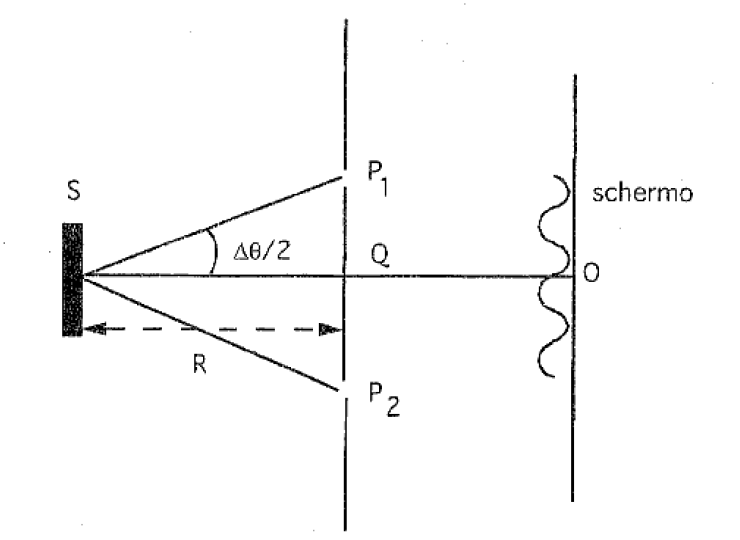
\includegraphics[width=0.6\textwidth]{Immagini/Young.png}
	\vspace{-10pt}
	\caption{}
	\label{fig:young}
	\vspace{-10pt}
\end{figure}

La presenza di frange sullo schermo è quindi è quindi una manifestazione della coerenza spaziale, infatti la capcità di due fasci di produrre frange è associata alla loro correlazione quando è introdotta una separazione spaziale, cioè quella data dalla distanza fra le sorgenti secondarie (vedi \cref{fig:young}).

Da un esperimento simile si può trovare che le frange si formano solo se la sorgente soddisfa la relazione:
\[ \Delta \theta \Delta s \leq \lambda \]
dove $ \Delta\theta $ è l'angolo sotto cui la sorgente vede le sorgenti secondarie, $ \lambda $ è la lunghezza d'onda dell'emissione. Per cui se la sorgente è a distanza $ R $ dal piano delle sorgenti secondarie le due sorgenti devono trovarsi entro un'area di ampiezza $ A_c $:
\[ A_c \simeq (R\Delta\theta_c)^2 = \frac{R^2\lambda^2}{S} \]
dove $ \Delta\theta_c $ è la quantità che satura la disuguaglianza precedente. La regione $ A_c $ è detta \textit{regione di coerenza} e la sua radice \textit{lunghezza di coerenza trasversale}. Si definisce anche l'\textit{angolo solido di coerenza}, come grandezza indipendente dalla distanza tra la sorgente e le sorgenti secondarie:
\[ \Delta\Omega = \frac{A_c}{R^2} = \frac{\lambda^2}{S} \]
C'è anche un altro angolo solido che può essere utile: quello sotteso dall'estensione della sorgente centrato nel punto medio fra le sorgenti secondarie, $ \Delta\Omega' $:
\[ S =  R^2 \Delta\Omega'\]
da cui si ottiene:
\[ A_c = \frac{\lambda^2}{\Delta\Omega'} \]

 \subparagraph{Interpretazione della coerenza spaziale} L'essenza della coerenza spaziale può essere tratta dalla seguente situazione: si immaginino due sorgenti puntiformi identiche spazialmente distanti e statisticamente indipendenti, \cref{fig:spcoh}.

\begin{figure}[h]
	\centering
	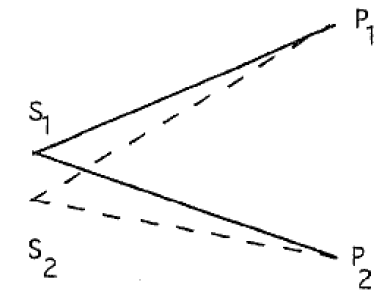
\includegraphics[width=0.4\textwidth]{Immagini/Spatialcoh.png}
	\vspace{-10pt}
	\caption{}
	\label{fig:spcoh}
	\vspace{-10pt}
\end{figure}

Si immaginino quindi due sorgenti secondarie come nel caso precedente, per le quali la differenza di cammino fra i fasci sia inferiore alla lunghezza di coerenza, $ c/\Delta\omega $, per entrambe le sorgenti. Si avrà allora che il valore dei campi prodotti nei due punti sarà lo stesso, a meno di un fattore di fase costante, dipendente dalla differenza di cammino.

Il campo totale sulle due sorgenti secondarie sarà la somma di due contributi statisticamente indipendenti. I due valori ottenuti, uno per sorgente secondaria, sono fortemente correlati: i singoli addendi differiscono solo per un termine di fase costante. In questo modo se anche le sorgenti primarie erano statisticamente indipendenti, quelle secondarie non lo sono affatto, e formano quindi una figura di interferenza sullo schermo.

\begin{oss}[Diffrazione]
	Si noti che la formula trovata per l'angolo solido di coerenza coincide con quella ottenuta per caratterizzare l'angolo solido di emissione di una sorgente diffrattiva secondaria di estensione $ S $, realizzata forando una parete opaca\footnote{Il contenuto di questa frase è che sostanzialmente non è interessante se la sorgente sia primaria o secondaria, a patto che nel secondo caso la radiazione incidente sia coerente (tipo onda piana)}.
	
	Perciò l'area di coerenza introdotta è una quantità che caratterizza i fenomeni diffrattivi dovuti all'estensione finita della sorgente.
\end{oss}

\begin{es}
	Si riportano alcuni esempi di aree di coerenza, sono omessi i calcoli.
	\begin{itemize}
		\item Sorgente d'onda termica con radiazione centrata a $ \lambda = \unit{500}{\nano\meter} $ e dimensione trasversale $ \Delta s = \unit{1}{\milli\meter} $. Per uno schermo a distanza $ R = \unit{2}{\meter} $ si ottiene $ A_c = \unit{1}{\milli\meter^2} $.
		\item Sole, con radiazione filtrata a $ \lambda = \unit{500}{\nano\meter} $. Si ottiene $ A_c \simeq \unit{3.7 \cdot 10^{-3}}{\milli\meter^2} $.
		\item Betelgeuse ($ \alpha $ di Orione), con radiazione filtrata a $ \lambda = \unit{500}{\nano\meter} $. Si ottiene $ A_c \simeq \unit{6}{\meter^2} $.
	\end{itemize}
\end{es}

Il prodotto tra l'area di coerenza $ A_c $ e la lunghezza di coerenza $ l_c $ determina un \textit{volume di coerenza}:
\[ V_c = A_c l_c = R^2 \frac{\lambda^2}{S} c \tau_c\]
e si può interpretare come la regione dello spazio in cui i fotoni sono indistinguibili gli uni dagli altri.

\subsubsection{Conteggio degli stati}

Si consideri ancora la sorgente descritta nell'esperienza di Young. Per il calcolo degli stati di singola particella si applica il procedimento descritto in \cref{sec:sumasint}: si calcola il volume di spazio delle fasi unitario e si divide per il volume della cella unitaria.

Il numero di stati è quindi:
\[ g = \frac{\Delta\Omega V p^2 \Delta p}{\hplanck^3} \]
in cui si è considerata una distribuzione isotropa in impulsi, e si selezionata la frazione a energia fissata, racchiusa nell'angolo solido di osservazione, mentre il volume $ V $ è dato dal volume occupato dai fotoni ricevuti nel tempo $ T $ di misura:
\[ V = S c T \]
L'impulso si trova a partire dall'energia dei singoli fotoni e dalla legge di dispersione:
\[ p = \frac{E}{c} = \frac{\hplanck\nu}{c} = \frac{\hbar \omega}{c} \]
Si ottiene quindi:
\[ g = \frac{\Delta\Omega S}{\lambda^2} \frac{T}{\tau_c} \]

\begin{defn}[Estensione del fascio]
	Si definisce \textit{estensione} di un fascio luminoso la quantità:
	\begin{equation*}
	U = \Delta\Omega S
	\end{equation*}
\end{defn}
La definizione di $ U $ è importante perché questa grandezza mantiene un valore costante nella propagazione di un fascio luminoso sotto le leggi dell'ottica geometrica.

Per il caso dell'angolo solido $ \Delta\Omega $ determinato dalla diffrazione della superficie $ S $ della sorgente si ottiene che l'estensione ha il valore $ U_c $:
\[ U_c = \frac{\lambda^2}{S} S = \lambda^2 \]
e quindi il numero degli stati è:
\[ g = \frac{U}{U_c} \frac{T}{\tau_c} \]
in cui il primo termine è definito \textit{fattore di coerenza spaziale} e il secondo \textit{fattore di coerenza temporale}.

\begin{oss}
	Il fattore di coerenza spaziale può essere scritto nella forma:
	\[ \frac{U}{U_c} = \frac{S'}{A_c} \]
	con $ S' = R^2 \Delta\Omega $ cioè l'area di osservazione. In questa forma tale fattore diventa analogo al fattore di coerenza temporale, cioè il rapporto tra una grandezza relativa all'osservazione e una grandezza caratterizzante le proprietà di coerenza della sorgente.
\end{oss}

Poiché $ g $ corrisponde a un numero intero, il cui minimo è $ 1 $, si ha che i due fattori di coerenza non possono mai essere minori di $ 1 $ individualmente (se uno dei due lo fosse si potrebbe portare a $ 1 $ l'altro riducendo $ g $ a un valore inferiore all'unità), per cui non possono essere utilizzati per compensarsi a vicenda.

Se i valori delle grandezze di osservazione sono maggiori di quelli delle grandezze di coerenza si otterrà una figura a contrasto più basso, perché i fotoni raccolti non sono tutti coerenti fra loro.

\begin{es}[Numero di stati]
	Il valore dell'\textit{estensione di coerenza} è determinato dalla sola lunghezza d'onda della radiazione raccolta. Considerando il valore degli esempi precedenti, $ \lambda = \unit{500}{\nano\meter} $, si ha $ U_c = \unit{25\cdot10^{-10}}{\centi\meter^2}$. Per una sorgente di $ S = 1 \milli\meter^2 $ posta a distanza $ R = 1 \meter $ da uno schermo di $ S' = 1 \centi\meter^2 $ si ottiene:
	\[ \frac{U}{U_c} = 400 \]
	Per cui bisognerebbe porsi molto più lontano per diminuire questo numero (infatti se lo schermo fosse più lontano diminuirebbe l'angolo solido sotteso). Per un valore pari a $ 1 $ per il fattore di coerenza occorrerebbe porsi a $ 20 \meter $ di distanza.
	
	\noindent La parte temporale è stata già discussa, infatti il periodo di osservazione andrà adeguato al tempo di coerenza $ \tau_c $.
\end{es}

\subsection{Interferometria stellare e di Hanbury Brown e Twiss}

L'interferometro di Hanbury Brown e Twiss è un'evoluzione dell'interferometro stellare di Michelson. Esso è stato usato per la misura dei \textit{raggi angolari} delle stelle viste dalla Terra.

\begin{figure}[b]
	\centering
	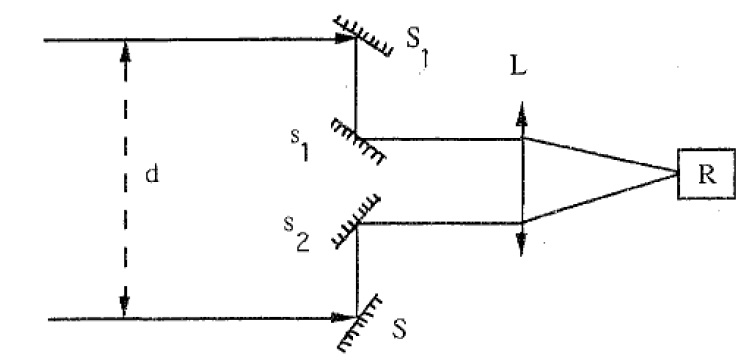
\includegraphics[width=0.6\textwidth]{Immagini/StellarMichelson.png}
	\vspace{-10pt}
	\caption{}
	\label{fig:michelsonst}
	\vspace{-10pt}
\end{figure}

\paragraph{Interferometro stellare di Michelson} Nell'interferometro di Michelson, \cref{fig:michelsonst}, la luce di una sorgente distante (una stella) arriva su due specchi primari $ S_1$ ed $ S_2 $, separati da una disanza $ d $ che può essere variata. La luce viene riflessa su due specchi secondari $ s_1$ ed $ s_2 $ e convogliata attraverso una lente $ L $ su  un rivelatore.

Finché i due specchi primari sono distanti meno di una lunghezza di coerenza trasversale (cioè appartengono alla stessa area di coerenza) il contrasto della figura di interferenza dipende solo dal fattore temporale. La condizione è quindi:
\[ d < \sqrt{A_c} = \frac{2}{\sqrt{\pi}}\frac{R \lambda}{a} = \frac{2}{\sqrt{\pi}}\frac{\lambda}{\alpha} \]
dove si è espressa l'area $ S $ della stella attraverso il suo diametro $ a $:
\[ S = \frac{\pi a^2}{4} \]
e il diametro angolare $ \alpha $ attraverso la distanza dalla Terra $ R $:
\[ \alpha = \frac{a}{R} \]
perciò testando la disuguaglianza per $ d $ si può misurare $ \alpha $.

\paragraph{Interferometro di Hanbury Brown e Twiss} Nel metodo di Hanbury Brown e Twiss si sostituiscono le due coppie di specchi (destra e sinistra) con due rivelatori, che forniscono dei segnali elettrici associati all'intensità luminosa (vedi \cref{fig:hbrowntwiss}).

\begin{figure}[t]
	\centering
	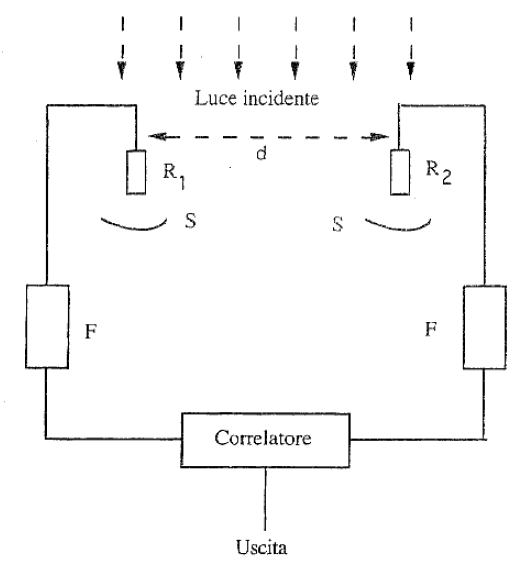
\includegraphics[width=0.6\textwidth]{Immagini/HanburyBrownTwiss.png}
	\vspace{-10pt}
	\caption{}
	\label{fig:hbrowntwiss}
	\vspace{-10pt}
\end{figure}

I segnali elettrici presentano fluttuazioni, che vengono esaminate attraverso il \textit{correlatore}. La misura si ottiene come nel caso di MIichelson variando la distanza $ d $ e misurando le correlazioni.

Siano quindi $ N_1, N_2 $ il numero dei fotoni che arrivano sui due rivelatori, e $ \overline{N_1}, \overline{N_2} $ i rispettivi valori medi. Il segnale di correlazione è definito come:
\[ C = (N_1 - \overline{N_1})  (N_2 - \overline{N_2}) \]
ed il correlatore fornisce la media di questa quantità, $ \overline{C} $. Se i rivelatori sono nella stessa area di coerenza (come nel caso di Michelson) il numero di possibili stati di singola particella è quindi $ g = T/\tau_c $, perché il fattore di coerenza spaziale è unitario.

Come descritto nella \cref{sec:fotonfluct}, questa volta però considerando anche il contributo corpuscolare, si ottiene per le fluttuazioni:
\[ \overline{(N_1 - \overline{N_1})^2} = \overline{N_1} + \frac{\overline{N_1}^2}{g} \]
e la stessa cosa si ottiene anche per $ N_2 $ e $ N = N_1 + N_2 $.

Esplicitando la relazione per $ N $ in termini di $ N_1,N_2 $ si ottiene:
\begin{align*}
\overline{(N_1 + N_2 - \overline{N_1 + N_2})^2} = \overline{N_1 + N_2} &+ \frac{\overline{N_1 + N_2}^2}{g}\\
\overline{(N_1 - \overline{N_1})^2} + \overline{(N_2 - \overline{N_2})^2} + 2 \overline{(N_1 - \overline{N_1})(N_2 - \overline{N_2})}& = \overline{N_1} + \frac{\overline{N_1}^2}{g} + \overline{N_2} + \frac{\overline{N_2}^2}{g} + 2 \frac{\overline{N_1}\overline{N_2}}{g}
\end{align*}
da cui, eliminando le relazioni trovate sopra per $ N_1, N_2 $, si ottiene l'espressione per la correlazione mediata sul tempo:
\[ \overline{C} = \overline{(N_1 - \overline{N_1})  (N_2 - \overline{N_2})} = \frac{\overline{N_1}\overline{N_2}}{g} \]

Quando i rivelatori vengono allontanati e la loro distanza supera la lunghezza trasversale di coerenza la formula per la correlazione media non è più valida, si può affermare però che essa diminuisce rapidamente.

\begin{oss}[Altre statistiche]
	La formula trovata vale per particelle che obbediscono alla statistica di Bose, per trovare l'espressione nel caso delle statistiche di Fermi e di Boltzmann è sufficiente modificare l'espressione per $ \overline{(N_1 - \overline{N_1})^2} $: nel primo caso al secondo membro il termine ondulatorio ha un segno meno, mentre nel caso classico è del tutto assente.
	
	Questo porta ad un segno $ - $ nella correlazione media dei fermioni, rispetto a quella dei bosoni, mentre porta ad annullarsi completamente la correlazione nel caso di particelle classiche.
\end{oss}

Per bosoni e fermioni il comportamento della correlazione media può essere spiegato in termine dei fenomeni di bunching e anti-bunching introdotto nella \cref{sec:fotonfluct}:
\begin{itemize}
	\item i bosoni tendono a raccogliersi insieme, per cui un aumento del numero di fotoni su un rivelatore indica un \textit{bunch} con più fotoni, per cui è probabile trovare più fotoni anche sull'altro;
	\item ai fermioni, a causa del principio di esclusione di Pauli, è proibito viaggiare insieme, per cui a un aumento dei fotoni su un rivelatore corrisponderà una diminuzione sull'altro.
\end{itemize}
I comportamenti discussi si possono anche pensare alla luce delle interazioni efficaci fra particelle quantistiche introdotte nella \cref{sec:fewdegas}.
\newline

Il vantaggio di questo esperimento rispetto a quello di Michelson è che impiegano i due rivelatori anziché uno solo si elimina il termine classico delle fluttuazioni e si misura solo quello quantistico.

Poiché cioè che si misura è il prodotto delle intensità sui due rivelatori l'uscita dipende dalla quarta potenza del campo elettrico.

\paragraph{Misura della coerenza temporale} Nella descrizione dell'esperimento si è detto che viene variata la distanza $ d $ al fine di trovare la coerenza spaziale del segnale (lunghezza di coerenza trasversale).
Si può però scegliere di tenere fissa la distanza $ d $, all'interno dell'area di coerenza, e introdurre un ritardo temporale all'uscita di uno dei due rivelatori, e misurare la coerenza temporale:
\[ \overline{C(\tau)} = \overline{(N_1(t) - \overline{N_1})  (N_2(t+\tau) - \overline{N_2})} \]

Si osserverà quindi una forte correlazione per ritardi $ \tau < \tau_c $, mentre la correlazione diminuirà quando il ritardo sarà maggiore del tempo di coerenza.

\`E quindi possibile caratterizzare in maniera completa le proprietà di coerenza della radiazione incidente.

\section{Rumore}

\subsection{Teorema di Nyquist}

Nel $ 1927 $ Johnson ha osservato che ai capi di un elemento generico di un circuito elettrico (tipicamente il più semplice: una resistenza) sono presenti della fluttuazioni nel segnale dovute alla temperatura finita del componente. Tali fluttuazioni sono perciò definite \textit{rumore termico} o \textit{Johnson}.
La spiegazione fu immediatamente fornita Nyquist, da cui il risultato teorico noto come \textit{teorema di Nyquist}.
\newline

L'enunciato del teorema è il seguente: si consideri una resistenza $ R $ alla temperatura $ T $, ai suoi capi verrà generata una tensione fluttuante che se misurata in una banda di frequenza $ \Delta f $ possiede un valore quadratico medio:
\[ \overline{V_{\Delta f}^2} = 4 R \kt \Delta f \]

Il teorema di Nyquist ha due importanti caratteristiche:
\begin{itemize}
	\item è valido per ogni circuito elettronico;
	\item è un primo esempio del teorema di fluttuazione-dissipazione: lega l'ampiezza delle fluttuazione all'elemento dissipativo $ R $ del sistema.
\end{itemize}

\begin{oss}[Dipendenza dalla banda passante]
	La dipendenza dell'ampiezza delle fluttuazioni dalla banda passante ha una motivazione evidente: una banda passante minore implica l'integrazione del segnale per tempi più lunghi. Se il segnale è a media nulla queste fluttuazioni saranno sempre più attenuate per tempi di integrazione sempre maggiori, poiché le fluttuazioni positive compenseranno quelle negative (per alte bande passanti il problema non si pone nemmeno: le alte frequenze sono fortemente smorzate dagli elementi capacitivi, per cui sono segnali deboli e soggetti ad ogni sorta di rumore).
\end{oss}

Si consideri una linea di trasmissione senza perdita di lunghezza $ l $ ed impedenza caratteristica $ R $, terminata da entrambi i lati da una resistenza di carico $ R $.
Tutti gli elementi sono a contatto con un bagno termico, che fissa la loro temperatura a $ T $. La situazione è schematizzata in \cref{fig:nyqline}.

\begin{figure}[b]
	\centering
	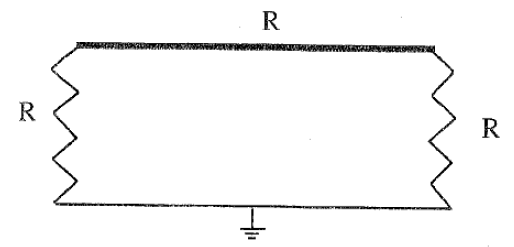
\includegraphics[width=0.6\textwidth]{Immagini/NyquistLine.png}
	\vspace{-10pt}
	\caption{}
	\label{fig:nyqline}
	\vspace{-10pt}
\end{figure}

Se si considera la propagazione di onde elettromagnetiche di lunghezza $ \lambda $ lungo tutta la linea. La linea presenta risonanze se:
\[ l = n \frac{\lambda}{2} \qquad \text{con}~n \in \mathbb{N} \]
Se $ c' $ è la velocità di propagazione lungo la linea si ha:
\[ l = n \frac{c'}{2 \nu} \implies n = l \frac{2\nu}{c'} \]
per cui in un intervallo di frequenza $ \Delta \nu $ ci saranno $ 2l \Delta \nu /c' $ modi di vibrazione.
Secondo la statistica di Bose ad ogni modo è associata un'energia:
\[ h\nu \bar{n} = h \nu \frac{1}{\exp[\frac{h\nu}{\kt}] - 1} \]
e nel limite classico $ h\nu \ll \kt $ l'energia diventa proprio $ \kt $. L'energia associata alla linea quindi risulta:
\[ h\nu \bar{n} \frac{2l}{c'} \Delta\nu \simeq \kt \frac{2l}{c'} \Delta\nu \]
e l'energia che si propaga per ogni direzione è la metà.

Questa energia viene portata alla resistenza in un tempo $ l/c' $, per cui la potenza per unità di tempo dissipata a carico della resistenza è:
\[ P_{\Delta\nu} = \kt \Delta\nu \]
Poiché si è all'equilibrio anche il carico $ R $ emette energia allo stesso ritmo, per cui la resistenza stessa genera alla temperatura $ T $ una potenza $ P_{\Delta\nu} $.

\begin{figure}[t]
	\centering
	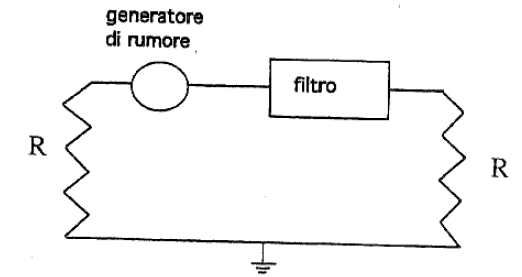
\includegraphics[width=0.6\textwidth]{Immagini/NyquistNoiseGenerator.png}
	\vspace{-5pt}
	\caption{}
	\label{fig:nyqgen}
	\vspace{-10pt}
\end{figure}

Il sistema può essere schematizzato sostituendo la linea di trasmissione con un generatore di rumore e un filtro per la banda di frequenza d'interesse, come mostrato in \cref{fig:nyqgen}.

Nella resistenza di carico scorre quindi una corrente $ I_{\Delta\nu} $ tale che la potenza sia quella prodotta dalla linea, cioè:
\[ I_{\Delta\nu}^2 R = \kt \Delta\nu \]
allora il generatore di rumore è un generatore di tensione $ V_{\Delta\nu} $ con:
\[ V_{\Delta\nu} = 2 R I_{\Delta\nu} \]
% non capisco perché il 2
e quindi:
\[ V_{\Delta\nu}^2 = 4 R \kt \Delta\nu \]
che è esattamente la tesi del teorema di Nyquist.

\paragraph{Generalizzazione ad impedenze complesse} Il teorema può essere generalizzato per impedenze complesse, semplicemente considerando un circuito costituito da tre elementi in serie: una resistenza $ R $, un'impedenza complessa $ Z = X + i Y $ e un filtro, che selezioni la banda d'interesse.

Sia $ \overline{V_{\Delta\nu}^2(R)} $ il quadrato della tensione di rumore prodotta da $ R $ in una banda di frequenza $ \Delta\nu $. La potenza dissipata in $ Z $ sarà:
\[ P_Z = \overline{\Re\{IZ\} \Re\{I\}} = \frac{1}{2} \Re\{(IZ) I^\ast\} = \frac{1}{2} ((IZ) I^\ast + (IZ)^\ast I) = \frac{1}{2}\abs{I}^2 (Z + Z^\ast) = \frac{\overline{V_{\Delta\nu}^2(R)}}{(R+X)^2 + Y^2}X\]
dove si è usato che:
\[ I = \frac{\overline{V_{\Delta\nu}^2(R)}}{R + X +iY} \]

Viceversa associando una tensione $ V_{\Delta\nu}(Z) $ di rumore all'impedenza $ Z $ si scrive la potenza dissipata in $ R $ come:
\[  P_R = \frac{\overline{V_{\Delta\nu}^2(Z)}}{(R+X)^2 + Y^2}R \]

Essendo all'equilibrio le due potenza scritte sopra devono essere uguali, per cui:
\[ \overline{V_{\Delta\nu}^2(Z)} R = \overline{V_{\Delta\nu}^2(R)} X \]
da cui si ricava facilmente il valore per $ \overline{V_{\Delta\nu}^2(Z)} $:
\[ V_{\Delta\nu}^2(Z) = 4 X \kt \Delta\nu\]

\begin{es}
	Per una temperatura pari a $ 293 \kelvin $, una banda di frequenza $ 1 \hertz $ e una resistenza di carico di $ 1 \mega\ohm $ si ottiene:
	\[ \sqrt{V_{\Delta\nu = 1}^2} = 0.127 \micro\volt \]
\end{es}

\subsection{Teorema di Wiener-Khintchine}

\subsection{Derivazione microscopica del Teorema di Nyquist}

\subsection{Shot noise}

\chapter{Cristalli}
\label{chap:crystals}

% !TEX encoding = UTF-8
% !TEX TS-program = pdflatex
% !TEX root = ../Appunti.tex

In questo capitolo viene affrontato il tema dei solidi. Questa affermazioni però apre uno spettro fin troppo ampio in confronto agli argomenti che verranno trattati, nei quali si discuterà delle proprietà dovute a un qualche tipo di reticolo cristallino.

Da qui il nome del capitolo.

\section{Il dilemma della capacità termica}

La spiegazione dell'andamento con la temperatura della capacità termica dei solidi, illustrata in \cref{fig:heatcap}, è uno dei successi della teoria quantistica, ottenuto già nell'ambito della \textit{old quantum theory}.

\begin{figure}[h]
	\centering
	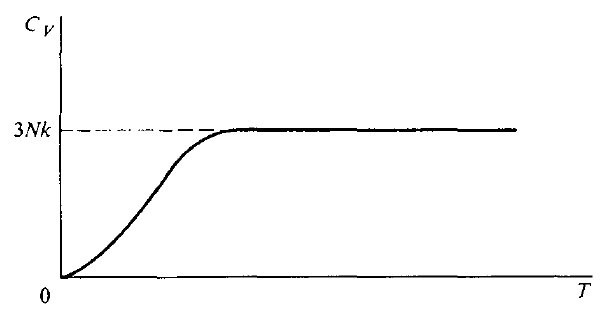
\includegraphics[width=0.6\textwidth]{Immagini/HeatCapacity.png}
	\vspace{-10pt}
	\caption{}
	\label{fig:heatcap}
\end{figure}

Si procederà esponendo i vari passaggi dell'evoluzione della teoria che sono stati compiuti storicamente: il teorema di equipartizione, il modello di Einstein e infine quello di Debye.

\subsection{Teorema di equipartizione}

Per studiare il comportamento degli atomi in un reticolo cristallino si introduce innanzi tutto l'\textit{approssimazione di campo medio}.

\begin{defn}[Campo medio]
	Si chiama \textit{approssimazione di campo medio} (o \textit{teoria}) un metodo che prevede di considerare, anziché per ogni particella le interazioni con ogni altra particella del sistema, solo un contributo mediato su tutte le altre particelle e incluso nella forma di un potenziale esterno in cui si trovi la singola particella in esame. 
\end{defn}

Nel caso in esame si considererà per ogni atomo del reticolo un potenziale efficace che lega il singolo atomo alla sua posizione di equilibrio.
Sia quindi $ \textbf{r} $ il vettore che indica lo spostamento dalla posizione di equilibrio, e $ u $ il potenziale efficace.
Poichè nella posizione di equilibrio non ci sono forze non bilanciate allora:
\begin{equation*}
	\partdev{u}{\textbf{\textbf{r}}} = 0	\qquad	\partdev{^2 u}{\textbf{\textbf{r}}^2} > 0
\end{equation*}
per cui si può espandere il potenziale efficace nel modo seguente:
\begin{equation*}
	u = u_0 + \frac{\alpha}{2} \textbf{r}^2
\end{equation*}
con $ \alpha = (\partial^2 u / \partial \textbf{r}^2)_{r=0} > 0 $. Con $ u_0 $ negativo, perché è l'energia di legame degli atomi ai siti dl reticolo.

Da tale potenziale si ottiene la legge di dispersione:
\begin{equation*}
	\varepsilon(\textbf{r}, \textbf{p}) = u_0 + \frac{\textbf{p}^2}{2m} + \frac{\alpha\textbf{r}^2}{2}
\end{equation*}

Per cui si ottiene per la funzione di partizione di singola particella:
\begin{align*}
	Z_1 &= \frac{1}{(\hplanck)^3} \int \cdots \int \exp[-\frac{\varepsilon(\textbf{p},\textbf{r})}{\kt}] \dd^3 p ~\dd^3 r =\\
	&= \frac{\exp(-u_0/\kt)}{(\hplanck)^3} \left[\int \exp(- \frac{p^2}{2 m \kt})\dd p\right]^3\left[\int \exp(- \frac{\alpha x^2}{2 \kt}) \dd x\right]^3
\end{align*}
Coefficienti a parte i due integrali che compaiono nell'espressione precedente sono identici:
\begin{equation*}
\int \exp(- \frac{a \xi^2}{\kt}) \dd xi = \frac{1}{2} \left(\frac{\kt}{a}\right)^{1/2} \int \eta^{1/2} e^{-\eta} \dd \eta
\end{equation*}

Riguardo i limiti di integrazione si nota che mentre per gli impulsi sono possibili tutti i numeri reali, per le posizioni ci si dovrebbe limitare ad una piccola area attorno alla posizione di equlibrio, che è quella in cui si è effettuato lo sviluppo.

Questo non è strettamente rilevante, infatti l'esponenziale si smorza fortemente anche per spostamenti non troppo grandi, per cui si può integrare anche qui da $ - \infty $ a $ + \infty $.

Si ha quindi per $ Z_1 $:
\begin{equation*}
	Z_1 = A (\kt)^3 \exp(-\frac{u_0}{\kt})
\end{equation*}
con $ A $ una costante (in cui è inclusa fra le altre cose la sesta potenza di $ \int_{0}^{\infty} \eta^{1/2} e^{-\eta} \dd \eta $).

Nonostante le considerazioni fatte nella \cref{sec:idpart} riguardo alle particelle identiche, qui non si hanno effetti di questo tipo poiché le particelle possono essere distinte in base al sito del reticolo che occupano. Per cui:
\begin{equation*}
Z = Z_1^N = A^N (\kt)^{3N} \exp(-\frac{N u_0}{\kt})
\end{equation*}
da cui si ricava l'energia libera:
\begin{equation*}
F = - \kt \log Z = N u_0 -3 N \kt \log\kt - N\kt \log A
\end{equation*}
e quindi l'entropia:
\begin{equation*}
S = - \partfix{F}{T}{V,N} = 3 N k_B \log\kt + 3 N k_B - N k_B \log A
\end{equation*}
e infine la capacità termica e l'energia:
\begin{align*}
C_V &= T \partfix{S}{T}{V,N} = 3 N k_B\\
E &= F + TS = 3 N \kt + N u_0
\end{align*}

I risultati ottenuti sono molto semplici e altrettanto chiari: l'energia è data dalla somma delle energie di legame di tutti gli atomi più il contributo termico per tutti i gradi di libertà.\footnote{La capacità termica trovata è nota come \textit{legge di Dulong-Petit.}}

Allo stesso modo la capacità termica è la somma dei contributi dei vari gradi libertà, $ 6 $ per ogni particella: $ 3 $ traslazionali e $ 3 $ vibrazionali. Il fatto più rilevante è che questo contributo sia pari a $ \frac{1}{2} k_B$ per ogni grado di libertà, indipendentemente dalla tipologia e dai dettagli del modello, per cui le costanti non entrano in gioco.

Questo è il contenuto del \textit{teorema di equipartizione}.

\begin{es}[Gas ideale]
	Nel modello di gas ideale i gradi di libertà erano solo 3, quelli traslazionali, e infatti la capacità termi trovata era $ \frac{3}{2} N k_B$.
\end{es}

Questo risultato è in accordo con i dati sperimentali ad alte temperature, ma non descrive l'andamento mostrato on \cref{fig:heatcap} per basse $ T $.

\subsection{Modello di Einstein}
\label{sec:einheatcap}

Il modello di Einstein è anch'esso una teoria di campo medio, in cui si considera un insieme di $ 3N $ oscillatori armonici indipendenti, esattamente come nel caso precedente.

L'unica differenza nelle ipotesi di partenza è nell'introduzione di un concetto quantistico: la \textit{quantizzazione dei livelli energetici} del singolo oscillatore.
\newline

Quanto scritto sopra si traduce in una enumerazione delle possibili energie del singolo oscillatore armonico:
\begin{align*}
	\varepsilon_\omega &= (n + 1/2) \hbar \omega + u_0/3 = \varepsilon_{0 \omega} + n \hbar \omega\\
	con &\qquad \varepsilon_{0 \omega} =  \frac{\hbar \omega}{2}  + \frac{u_0}{3}
\end{align*}
dove $  \varepsilon_{0 \omega} $ è l'energia del fondamentale. Come nel paragrafo precedente la frequenza è la stessa per tutti gli oscillatori.

La funzione di partizione del singolo oscillatore è:
\begin{equation*}
	Z_{1\omega} = \exp(-\frac{ \varepsilon_{0 \omega}}{\kt}) \sum_n \left[\exp(-\frac{ \hbar \omega}{\kt})\right]^n = \frac{\exp(- \varepsilon_{0 \omega}/\kt)}{1 - \exp(- \hbar \omega/\kt)}
\end{equation*}

Poiché i $ 3N $ oscillatori armonici sono tutti identici e indipendenti è sufficiente trovare le proprietà termodinamiche di singolo oscillatore, le altre si ottengono per estensività:
\begin{align*}
	F_{1\omega} &= - \kt \log Z_{1\omega}  = \varepsilon_{0 \omega} + \kt \log \left[1 - \exp(-\frac{ \hbar \omega}{\kt})\right]\\
	S_{1\omega} &= - k_B \log \left[1 - \exp(-\frac{ \hbar \omega}{\kt})\right]  + \frac{\hbar \omega}{T} \frac{\exp(- \hbar \omega/\kt)}{1 - \exp(- \hbar \omega/\kt)}\\
	E_{1\omega} &= 	F_{1\omega} + T S_{1\omega} = \varepsilon_{0 \omega} + \bar{n} \hbar \omega\\
	\bar{n} &= \frac{\exp(- \hbar \omega/\kt)}{1 - \exp(- \hbar \omega/\kt)} = \frac{1}{\exp(\hbar \omega/\kt) - 1}
\end{align*}
si noti che $ \bar{n} $ coincide con il numero di occupazione medio di ogni stato di singola particella di un gas di Bose degenere ($ \mu = 0 $); questa corrispondenza non è casuale.

Quindi per valutare le proprietà termodinamiche dell'intero sistema si moltiplicano per $ 3N $ quelle trovate per il singolo oscillatore. In particolare, per la capacità termica:
\begin{equation*}
	C_V = \partfix{E}{T}{V} = 3N \partfix{E_{1\omega}}{T}{V} = 3 N k_B \left(\frac{\hbar \omega_E}{\kt}\right)^2 \frac{\exp(\hbar \omega_E/\kt)}{[\exp( \hbar \omega_E/\kt) - 1]^2}
\end{equation*}
dove si è indicata con $ \omega_E $ la frequenza propria degli oscillatori, che sarà una proprietà del materiale. Si definisce frequentemente la temperatura di Einstein $ \Theta_E $:
\begin{equation*}
	k_B \Theta_E = \hbar \omega_E
\end{equation*}
in termini della quale si può riscrivere l'espressione della capacità termica.

Ad alte temperature, $ T \gg \Theta_E $, si ha per la capacità termica, approssimando al primo ordine:
\begin{equation*}
	C_V \rightarrow 3N k_B
\end{equation*}
cioè il risultato classico.
Nel limite opposto si ottiene invece:
\begin{equation*}
C_V \rightarrow 3N k_B \left(\frac{\hbar \omega_E}{\kt}\right)^2 \exp(-\frac{\hbar \omega_E}{\kt})
\end{equation*}
cioè che $ C_V \rightarrow_{T \rightarrow 0} ~0 $, che è in accordo con quanto mostrato in \cref{fig:heatcap}.

Questo risultato poteva essere previsto dalla meccanica quantistica: a temperatura $ T \rightarrow 0 $ il sistema si trova nel fondamentale, e la probabilità di eccitazione va a $ 0 $ con la temperatura, poiché $ \partial S / \partial T $ è finito.
\newline

Il modello di Einstein presenta un paio di incongruenze rispetto alle proprietà di un cristallo reale:
\begin{itemize}
	\item La capacità termica si annulla troppo rapidamente per $ T \rightarrow 0 $, infatti in questo limite si trova sperimentalmente:
	\begin{equation*}
	C_V \propto T^3
	\end{equation*}
	
	Il fatto che il modello di Einstein presenti un andamento esponenziale è dovuto alla struttura dei livelli energetici, in particolare alla presenza di un \textit{gap} finito tra il fondamentale e il primo eccitato.
	A causa di questa separazione se l'energia termica a disposizione diminuisce la probabilità di eccitazione decresce esponenzialmente, e quindi anche la capacità termica.
	\item L'altro problema è dato dai parametri del materiale $ u_0, \omega_E $. In una teoria di campo medio consistente queste quantità non possono dipendere dalla spaziatura tra gli atomi, poiché se così fosse il moto di un atomo influenzerebbe il vicino ed essi non sarebbero indipendenti.
	
	La spaziatura tra gli atomi non è altro che l'inverso della densità, e la richiesta che i parametri non dipendano dalla densità, e quindi dal volume se il numero di particelle è fissato, implica che:
	\begin{equation*}
		P = - \partfix{F}{V}{T,N} = 0
	\end{equation*}
	poiché la $ F $ dipende solo dalla $ F $ di singolo oscillatore, che contiene solo l'informazione sui parametri, e dal numero di oscillatori presenti.
	
	Analogamente la compressibilità isoterma diverge:
	\begin{equation*}
	K_T = - \frac{1}{V} \partfix{V}{P}{T,N} = - \left[V \partfix{^2 F}{V^2}{T,N}\right]^{-1}
	\end{equation*}	
\end{itemize}

Ovviamente in un cristallo reale il potenziale su un atomo dipende dalla posizione dei vicini, e quindi non sono indipendenti. La cosa inattesa è che migliorando il modello per risolvere il secondo punto anche il comportamento della capacità termica diventa quello corretto.

Si consideri un cristallo a temperatura nulla: esso sarà nel fondamentale e i suoi atomi saranno disposti in un reticolo regolare per minimizzare l'energia.
Non appena si inserisce un minimo di energia nel sistema, aumentando così la temperatura, ogni possibile tipo di eccitazione ne acquisirà una parte proporzionale a $ e^{-\mathcal{E}/\kt} $, dove $ \mathcal{E} $ è l'energia dell'eccitazione, e quindi ognuna contribuirà alla capacità termica con un termine proporzionale a $ e^{-\mathcal{E}/\kt} $. Per cui più piccola sarà $ \mathcal{E} $, più grande sarà il contributo alla capacità termica.

Si cerca quindi di costruire il primo livello eccitato del sistema, che sarà quello che maggiormente contribuirà alla capacità termica.

Si immagini di spostare un atomo dalla sua posizione di equlibrio: questo aumenterà la sua energia e quella dei suoi vicini. Per ottenere una configurazione a energia più bassa si può pensare di spostare anche i vicini in modo solidale, e quindi i loro vicini, \dots.
Se si estende questo procedimento a tutto il cristallo si è semplicemente spostato il suo centro di massa, senza modificare le posizioni relative, e quindi l'energia del sistema (in assenza di campi esterni ci sarà invarianza per traslazioni globali).

Per ottenere un risultato significativo anziché spostare solidalmente ogni atomo e i suoi vicini si può applicare ai vicini uno spostamento coerente, ma leggermente ridotto, in modo che le distanze relative cambino poco fra primi vicini.
Più esplicitamente, si pensi a un cristallo unidimensionale finito: si tengono fermi gli estremi, e partendo da uno dei due si aumenta gradualmente lo spostamento di ogni atomo dalla sua posizione di equilibrio, per poi diminuirlo  non appena superata la metà.

In questo modo si ottengono le onde sonore nei cristalli.
\newline

Dal risultato ottenuto si evince che la capacità termica a bassa temperatura è dominata dai modi collettivi del sistema, piuttosto che da quelli incoerenti come nel caso del modello di Einstein.

Si possono pensare questi modi organizzati come nel caso del modello di Einstein: un insieme di $ 3N $ oscillatori indipendenti, ciò che differisce dal caso precedente è che la frequenza non è unica, ma dipende dal modo considerato.

\begin{defn}[Modi normali]
	I modi collettivi descritti sono detti \textit{modi normali} e sono quelli che diagonalizzano l'Hamiltoniano del sistema (proprio per questo sono indipendenti).
\end{defn}

Le proprietà termodinamiche saranno quindi saranno calcolate in modo simile a quelle del modello di Einstein, ma per ottenere il risultato sarà necessario conoscere la distribuzione in frequenza dei modi normali.
\begin{align*}
	F &= E_0 + \kt \sum_\alpha \log \left[1 - \exp(-\frac{\hbar \omega_\alpha}{\kt})\right]\\
	E &= E_0 + \sum_{\alpha} \bar{n}_\alpha \hbar \omega_\alpha\\
	\text{con}	&\qquad  \bar{n}_\alpha = \frac{1}{\exp(\bar{n}_\alpha/\kt) - 1}
\end{align*}

\subsubsection{Numero di modi normali}

Il modo più corretto per capire quanti modi normali ci siano è esaminare la struttura delle equazioni, e si ottiene facilmente che se le equazioni in campo medio hanno $ 3N $ soluzioni, corrispondenti al numero di oscillazioni indipendenti, allora modificando le equazioni si otterrano soluzioni più complicate, ma il numero sarà sempre lo stesso per i teoremi generali sulla teoria delle equazioni differenziali lineari.
\newline

C'è un altro modo però per ottenere tale numero nel caso del modello considerato, esaminando il limite per alte $ T $, cioè il limite classico.

In tale limite il sistema soddisfa le ipotesi del teorema di equipartizione, e quindi studiando il valore dell'energia:
\begin{align*}
 \bar{n}_\alpha &\simeq \frac{\kt}{\hbar \omega_\alpha} \implies  \bar{n}_\alpha \hbar \omega_\alpha \simeq \kt \implies \\
 &\implies E \simeq E_0 + \tilde{N} \kt
\end{align*}
è lo stesso teorema di equipartizione a imporre $ \tilde{N} = 3N  $, dove $ \tilde{N} $ è il numero di modi normali.

\subsection{Modello di Debye}

Quanto detto nella \cref{sec:einheatcap} a proposito delle onde sonore è alla base del modello di Debye. Si procederà quindi ricavando prima la legge di dispersione per basse frequenze, in modo da poter determinare il comportamento a bassa temperatura della capacità termica.

\subsubsection{Legge di dispersione per onde lunghe}

Nei cristalli le onde sonore hanno $ 3 $ polarizzazioni, due trasverse e una longitudinale, cui corrispondono anche due diverse velocità $ c_t $ e $ c_l $.
Per semplificare la trattazione si considererà solamente quella longitudinale.
Il risultato ottenuto sarà comunque applicabile esattamente per i liquidi\footnote{Essi non hanno polarizzazioni trasverse, perché gli strati scorrono l'uno sull'altro.}.
\newline

\noindent Poiché si sta cercando il comportamento delle onde lunghe si può trascurare la struttura atomica, e considerare il mezzo come un continuo.

Dalla legge di Newton si ricava:
\begin{equation*}
\partdev{P}{x} + \rho\partdev{v}{t} = 0
\end{equation*}
mentre dalla conservazione della massa:
\begin{equation*}
\partdev{\rho}{t} + \partdev{\rho v}{x} = 0
\end{equation*}
dove in entrambe $ \rho $ è la densità, $ P $ la pressione, $ t $ il tempo, $ x $ la coordinata spaziale e $ v $ la velocità.

Poiché si cerca il comportamento per piccoli spostamenti dalle posizioni di equilibrio è utile definire le equazioni proprio in termini di queste variazioni:
\begin{align*}
P &= P_0 + P'\\
\rho &= \rho_0 + \rho'\\
v &= v'
\end{align*}
e scrivendo le equazioni al prim'ordine in questi spostamenti (cioè eliminando i termini in cui compaiono più di un fattore primao):
\begin{equation*}
\begin{cases*}
\partdev{P'}{x} + \rho_0 \partdev{v'}{t} = 0\\
\partdev{\rho'}{t} + \rho_0 \partdev{v'}{x} = 0
\end{cases*}
\end{equation*}

Si hanno perciò tre incognite e due equazioni. Per risolvere questo problema si considera quindi che la densità sia una funzione della sola pressione $ \rho \equiv \rho(P) $, e di conseguenza:
\begin{equation*}
\rho = \rho(P_0) + \partdev{\rho}{P} P' \qquad \implies \qquad \rho' = \partdev{\rho}{P} P' = \frac{1}{c^2} P'
\end{equation*}
dove si è definito\footnotemark:
\footnotetext{Si ha infatti:
	\begin{equation*}
	\partfix{\rho}{P}{N,T/S} = \partfix{N/V}{P}{N,T/S} = - \frac{N}{V^2} \partfix{V}{P}{N,T/S} = \rho K_{T/S}
	\end{equation*}
}
\begin{equation*}
c^2 = \partdev{P}{\rho} = \frac{1}{K \rho}
\end{equation*}
Nell'equazione di stato la densità dipende sia dalla pressione che dalla temperatura. ignorare la dipendenza dalla temperatura corrisponde a ignorare la differenza tra $ C_P $ e $ C_V $, o tra $ K_T $ e $ K_S $, che è una buona approssimazione per i mezzi continui, dove le compressibilità sono piccole\footnote{Nella \cref{sec:thermdev} si è trovato infatti che la differenza delle capacità termiche è proporzionale al quadrato di $ (\partial V / \partial T)_P $.}. Perciò il $ K $ che appare nell'espressione precedente è indifferente quale sia.

Si ottengono quindi le equazioni:
\begin{equation*}
\begin{cases*}
c^2\partdev{\rho'}{x} + \rho_0 \partdev{v'}{t} = 0\\
\partdev{\rho'}{t} + \rho_0 \partdev{v'}{x} = 0
\end{cases*}
\end{equation*}
e prendendo $ \partial/\partial x $ della prima e $ \partial/\partial t $ della seconda e sottraendo si ha:
\begin{equation*}
	\partdev{^2\rho}{x^2} - \frac{1}{c^2} \partdev{^2\rho}{t^2} = 0
\end{equation*}
che è la nota equazione di D'Alembert che ammettono soluzioni propaganti con una legge di dispersione lineare.
\begin{equation*}
	\omega = \pm c q
\end{equation*}

Si ottiene infine che $ \omega $ assume un insieme di valori discreto, determinato dall'insieme di valori discreto che può assumere $ q $, fissando, ad esempio, condizioni periodiche al contorno:
\begin{equation*}
	\rho'(x=0) = \rho'(x=L)
\end{equation*}
che implicano per $ q $:
\begin{equation*}
	q = \frac{2\pi}{L}n
\end{equation*}
dove $ n $ è un numero intero, limitato dall'alto (se avessimo la legge di dispersione esatta il limite sarebbe fissato dal passo reticolare, ma poiché si sta trattando il caso di onde lunghe il limite è fissato dagli estremi di validità  dell'approssimazione).

\subsubsection{Capacità termica e proprietà termodinamiche}

Si applica quindi il risultato trovato per la legge di dispersione, distinguendo però le tre polarizzazioni. Per farlo si indica la generica velocità con $ c_i $, $ i = l,t $.
\newline

Poiché il numero di modi per ogni polarizzazione è molto grande, dell'ordine di $ N $, le somme possono essere convertite in integrali, per cui anche l'enumerazione dei modi va trasformata in una densità di modi.

Per l'enumerazione si aveva:
\begin{align*}
	\textbf{q} &= \left(\frac{2\pi}{L}\right) \textbf{n}\\
	\text{con} &\qquad \textbf{n} = n_1 \hat{\textbf{x}} + n_2 \hat{\textbf{y}} + n_3 \hat{\textbf{z}}
\end{align*}
e poiché il cristallo immaginato ha dimensione $ L $ per ogni lato si ha $ V = L^3 $. Il numero di modi compreso tra $ \textbf{n} $ e $ \textbf{n} + \dd \textbf{n} $, cioè $ \dd \textbf{n} $, è quindi un differenziale tridimensionale $ \dd \textbf{n} = \dd^3 n $.

Il numero di modi compresi tra $ \textbf{q} $ e $ \textbf{q} + \dd \textbf{q} $ è:
\begin{align*}
	\dd^3 n &= \frac{V}{(2\pi)^3} \dd^3 q \implies\\
	&\implies \dd^3 n = \frac{4\pi V q^2 \dd q}{(2\pi)^3}
\end{align*}
in cui nella seconda si è assunto che il solido sia isotropo.

Dalla legge di dispersione si ottiene infine:
\begin{equation*}
	\rho_i(\omega) \dd \omega = \frac{4\pi V}{(2\pi)^3} q(\omega)^2 \dd q(\omega) = \frac{4\pi V}{(2\pi c_i)^3} \omega^2 \dd \omega
\end{equation*}
La densità di modi ha lo stesso ruolo che la densità di stati di singola particella aveva nel \cref{chap:gas}. La differenza principale tra i due casi sta proprio nella legge di dispersione, che implica una diversa densità, esattamente come si era trovato nell'\cref{es:lindisp}.

Inoltre il ruolo del numero di particelle nello stato (numero di occupazione) è qui assunto dal numero di eccitazioni di un certo oscillatore.

Tutte queste analogie portano a definire l'eccitazione elementare come una particella, o meglio una \textit{quasiparticella} (vedi \cref{sec:idpart}), e trattare l'insieme degli oscillatori come un gas perfetto di eccitazioni non interagenti: nei cristalli sono dette \textit{fononi}.
\newline

Se il cristallo è isotropo le due polarizzazioni trasverse hanno la stessa velocità di propagazione, e sommando sulle tre polarizzazioni si ottiene:

\begin{equation*}
\rho(\omega) \dd \omega = \frac{4\pi V}{(2\pi)^3}\left(\frac{1}{c_l^3} + \frac{2}{c_t^3}\right) \omega^2 \dd \omega
\end{equation*}
e definendo:
\begin{equation*}
	\frac{3}{\tilde{c}^3} = \frac{1}{c_l^3} + \frac{2}{c_t^3}
\end{equation*}
si ha:
\begin{equation*}
\rho(\omega)= \frac{12\pi V}{(2\pi\tilde{c})^3}\omega^2 
\end{equation*}

La formula trovata è stata ricavata assumendo la legge di dispersione per onde lunghe, quindi è valida solo nel limite di bassa frequenze, ma a bassa temperatura, cioè se $ \omega $ è abbastanza grande tale che:
\begin{equation*}
\hbar \omega \gg \kt
\end{equation*}
allora è il numero di eccitazioni a essere esponenzialmente smorzato (vedi \cref{sec:einheatcap}), per cui anche estendendo l'integrale fino a $ \infty $ si commette un errore piccolo.

Si ha quindi per l'energia:
\begin{align*}
	E_{th} = \int_{0}^{\infty} \bar{n}(\omega)\rho(\omega) \hbar \omega \dd \omega = \frac{12\pi V}{(2\pi\tilde{c})^3}\hbar \int_{0}^{\infty} \frac{\omega^3 \dd \omega}{\exp(\hbar\omega/\kt)-1} = \frac{12\pi V}{(2\pi\hbar\tilde{c})^3} (\kt)^4 \int_{0}^{\infty} \frac{x^3 \dd x}{e^x -1}
\end{align*}
L'integrale definito può essere valutato e risulta essere pari a $ \pi^4 / 15 $.

La cosa più importante è che la dipendenza dell'energia è $ E \propto T^4 $ e di conseguenza $ C_V = \partfix{E}{T}{V} \propto T^3$, cioè l'andamento sperimentalmente verificato.
\newline

Si sono trascurati del tutto i modi ad alta frequenza, per cui non è stata neanche trovata la legge di dispersione. Essi però non contribuiscono sostanzialmente in nessuno dei due limiti: per basse temperature sono i coinvolti solo i modi a bassa frequenza, perché quelli ad alta frequenza sono congelati, mentre per temperature alte il teorema di equipartizione impone che l'unica informazione rilevante sia il numero di modi.

Per questo è naturale raccordare i due andamenti semplicemente estendendo il limite di validità della densità di modi e considerando $ \rho(\omega) \propto \omega^2 $ fino a una certa frequenza massima $ \omega_m $ fissata da:
\begin{equation*}
	3N = \int_0^{\omega_m} \rho(\omega) \dd \omega
\end{equation*}
tale interpolazione è proprio ciò che viene chiamato \textit{modello di Debye}.

La frequenza massima $ \omega_m $ è come $ \omega_E $ nel modello di Einstein una proprietà del materiale, e può essere espresso per mezzo della velocità media di propagazione del suono e della densità del materiale:
\begin{equation*}
	\omega_m = 2 \pi \tilde{c} \left(\frac{3N}{4\pi V}\right)^{1/3}
\end{equation*}

Si sarebbe potuto decidere di porre il cutoff in un altro modo, ad esempio facendolo in modo ditinto per ogni polarizzazione, che va pure bene, ma a questo livello è una complicazione non necessaria.

Come nel caso di Einstein anche qui si può definire una temperatura caratteristica, detta \textit{temperatura di Debye} $ \Theta_D $:
\begin{equation*}
\hbar \omega_m = k_B \Theta_D
\end{equation*}
e riportando in un grafico (come in \cref{fig:heatcapdeb}) $ C_V/N k_B $ contro $ T/\Theta_D $ si otttiene un andamento universale, coerente con i dati sperimentali, contrariamente alla \cref{fig:heatcap}.
\newline

\begin{figure}[h]
	\centering
	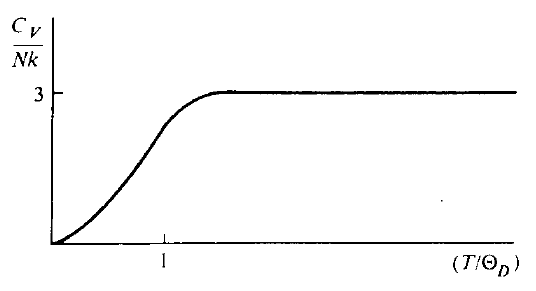
\includegraphics[width=0.6\textwidth]{Immagini/HeatCapacityDebye.png}
	\vspace{-10pt}
	\caption{}
	\label{fig:heatcapdeb}
\end{figure}

Per evidenziare la natura quasiparticellare dei fononi si descrivono in termini delle stessa grandezze tipiche delle particelle:
\begin{align*}
	\varepsilon &= \hbar \omega \qquad p = \hbar q\\
	\varepsilon &= \tilde{c} p \qquad \rho(\varepsilon) \dd \varepsilon =  3 \frac{4\pi V}{(2\pi)^3} p^2 \dd p \iff 
	\rho(\varepsilon)= \frac{12\pi V}{(2\pi\tilde{c})^3}\varepsilon^2 
\end{align*}
il fattore $ 3 $ è inserito nell'ultima equazione per contare le polarizzazione, e corrisponde in modo non ancora evidente alla degenerazione di spin.

Non ci sono limiti all'occupazione di un dato stato per i fononi, quindi essi seguono la statistica di Bose. Il numero di particelle non è fissato, ma libero di fluttuare ed esso cerca di minimizzare l'energia libera, per cui:
\begin{equation*}
\mu_{ph} = \partfix{F}{n_{ph}}{T,V} = 0
\end{equation*}
per cui i fotoni si comportano come il \textit{vapore di Bose}, cioè la parte non condensata di un gas totalmente degenere, da cui il numero di occupazione è:
\begin{equation*}
\bar{n} = \frac{1}{\exp(\varepsilon/\kt)}
\end{equation*}

Si possono quindi usare le formule del gas perfetto per trovare le proprietà termodinamiche. Si esprime innanzi tutto la densità di stati in funzione della temperatura di Debye piuttosto che della velocità del suono:
\begin{align*}
&\begin{rcases*}
\rho(\varepsilon) = A \varepsilon^2\\
3N = \int_0^{k_B \Theta_D} \rho(\varepsilon) \dd \varepsilon
\end{rcases*}
3N = A \int_0^{k_B \Theta_D} \varepsilon^2 \dd \varepsilon \implies\\
&\implies \rho(\varepsilon) = \frac{9N}{(k_B \Theta_D)^3}\varepsilon^2
\end{align*} 
per cui si ha per l'energia:
\begin{equation*}
E_{th} = \int_0^{k_B \Theta_D} \varepsilon \rho(\varepsilon) \bar{n}(\varepsilon)\dd \varepsilon = 9 N \kt \left(\frac{T}{\Theta_D}\right)^3  \int_0^{k_B \Theta_D} \frac{x^3 \dd x}{e^x -1}
\end{equation*}
dove l'ultimo integrale dipende da $ T $ tramite l'estremo superiore, e in generale non può essere fatto analiticamente. A basse temperature, cioè $ T \ll \Theta_D $ il limite superiore può essere rimpiazzato da $ + \infty $ e si ottiene:
\begin{align*}
E_{th} &= \frac{3}{5} \pi^4 N \kt \left(\frac{T}{\Theta_D}\right)^3\\
C_V &= \frac{12}{5} \pi^4 N k_B \left(\frac{T}{\Theta_D}\right)^3
\end{align*}
mentre nel limite opposto  $ T \gg \Theta_D $ il denominatore dell'integrando può essere espanso e $ e^x -1 \simeq x $, per cui l'integrale diventa facilmente svolgibile e si ottine:
\begin{equation*}
E_{th} = 3 N \kt
\end{equation*}
che verifica la coerenza con quanto imposto.

\appendix

% per la parte di struttura dei liquidi si può rimandare direttamente alle slide

% TODO: Forse dovrei decidermi a imparare a usare la bibliografia di LaTeX

\end{document}